\documentclass[10pt,letterpaper,twoside,openright]{book}
\usepackage{amsmath}
\usepackage{graphicx}
\usepackage{amssymb}
\usepackage{cite}
\usepackage{todonotes}
\usepackage{etoolbox}
\usepackage{bbm}
\usepackage{booktabs}
\usepackage{csquotes}

\usepackage{graphicx}
\usepackage{tikz}
\usepackage{amssymb}
\usepackage{amsmath}
\usepackage{amsthm}
\usepackage{subfig}
%\usepackage{flushend}
\usepackage{nicefrac}
\usepackage{dsfont}
\usepackage{array}
\usepackage[vlined,ruled,linesnumbered]{algorithm2e}
\usepackage{booktabs}
\usepackage{url}


\newtheorem{example}{Example}
\newtheorem{definition}{Definition}
\usepackage{tikz}
\usetikzlibrary{backgrounds,calc,decorations.pathreplacing,matrix,arrows}
\usetikzlibrary{circuits,shapes}


\hyphenation{op-tical net-works semi-conduc-tor}


\newcolumntype{C}{>{$}c<{$}}
\newcolumntype{L}{>{$}l<{$}}
\newcolumntype{R}{>{$}r<{$}}

%\usepackage[disable
% ,backgroundcolor=yellow!30!white ,bordercolor=gray
  %,textsize=footnotesize
%]{todonotes}





\newcommand{\field}[1]{\ensuremath{\mathds{#1}}}
\newcommand{\B}{\field{B}}
\newcommand{\C}{\field{C}}
\newcommand{\N}{\field{N}}


\newcolumntype{C}{>{$}c<{$}}
\newcolumntype{L}{>{$}l<{$}}
\newcolumntype{R}{>{$}r<{$}}

%\usepackage[disable]{todonotes}
\usepackage{todonotes}


\def\crossbarpfheight{0.25}
\def\crossbarqgheight{0.90}
\def\crossbarcrossing{0.3}
\def\crossbarlineoutside{0.7}

% functional block
\def\functionalblockpfheight{0.25}
\def\functionalblockqgheight{0.90}
\def\functionalblocklineoutside{0.7}

\newlength{\crossbarheight}
\newlength{\crossbarwidth}
\newlength{\crossbarvarmargin}
\newlength{\defaultpgflinewidth}
\newlength{\combinersize}

%functional block
\newlength{\functionalblockheight}
\newlength{\functionalblockwidth}
\newlength{\functionalblockvarmargin}
%\newlength{\defaultpgflinewidth}

\setlength{\crossbarheight}{2em}
\setlength{\crossbarwidth}{1.5em}
\setlength{\crossbarvarmargin}{1.2em}
\setlength{\combinersize}{10pt}

%  functional block

\setlength{\functionalblockheight}{2em}
\setlength{\functionalblockwidth}{1.5em}
\setlength{\functionalblockvarmargin}{1.2em}


\makeatletter

\pgfdeclareshape{oldcrossbargate}{

 	\nodeparts{}
	\inheritanchorborder[from=rectangle]
	\inheritsavedanchors[from=rectangle]	
	
	
	\savedanchor{\varpos}{
		\pgf@x=0\crossbarwidth
		\pgf@y=0.8\crossbarheight
	}

	\savedanchor{\northeast}{
		\pgf@x=0.5\crossbarwidth
		\pgf@y=0.5\crossbarheight
	}
	\savedanchor{\southwest} {
		\pgf@x=-\pgf@x
		\pgf@y=-\pgf@y
	}
	
	\savedanchor{\p}{
		\pgf@x=-\crossbarlineoutside\crossbarwidth
		\pgf@y=0.2\crossbarheight
	}
	
	\savedanchor{\q}{
		\pgf@x=-\crossbarlineoutside\crossbarwidth
		\pgf@y=-0.2\crossbarheight
	}	
	
	\savedanchor{\f}{
		\pgf@x=\crossbarlineoutside\crossbarwidth
		\pgf@y=0.2\crossbarheight
	}
	
	\savedanchor{\g}{
		\pgf@x=\crossbarlineoutside\crossbarwidth
		\pgf@y=-0.2\crossbarheight
	}
	
	\savedanchor{\pcross}{
		\pgf@x=-0.25\crossbarwidth 
		\pgf@y=0.2\crossbarheight
	}
	
	\savedanchor{\qcross}{
		\pgf@x=-0.25\crossbarwidth 
		\pgf@y=-0.2\crossbarheight
	}	
	
	\savedanchor{\fcross}{
		\pgf@x=0.25\crossbarwidth 
		\pgf@y=0.2\crossbarheight	
	}
	
	\savedanchor{\gcross}{
		\pgf@x=0.25\crossbarwidth 
		\pgf@y=-0.2\crossbarheight
	}
	
	
	\anchor{f}{\f}
	\anchor{g}{\g}
	\anchor{p}{\p}
	\anchor{q}{\q}
	\anchor{fcross}{\fcross}
	\anchor{gcross}{\gcross}
	\anchor{pcross}{\pcross}
	\anchor{qcross}{\qcross}
	\anchor{varpos}{\varpos}
	\anchor{center}{\pgfpointorigin}
	
	\backgroundpath{
		% store lower right in xa/ya and upper right in xb/yb
		\southwest \pgf@xa=\pgf@x \pgf@ya=\pgf@y
		\northeast \pgf@xb=\pgf@x \pgf@yb=\pgf@y


		% rectangle
		\pgfpathmoveto{\pgfpoint{\pgf@xa}{\pgf@ya}}
		\pgfpathlineto{\pgfpoint{\pgf@xa}{\pgf@yb}}
		\pgfpathlineto{\pgfpoint{\pgf@xb}{\pgf@yb}}
		\pgfpathlineto{\pgfpoint{\pgf@xb}{\pgf@ya}}
		\pgfpathlineto{\pgfpoint{\pgf@xa}{\pgf@ya}}
		\pgfusepath{draw}
		
		
		% Bars
		\p \pgf@xa=\pgf@x \pgf@ya=\pgf@y
		\f \pgf@xb=\pgf@x \pgf@yb=\pgf@y
		\pgfpathmoveto{\pgfpoint{\pgf@xa}{\pgf@ya}}
		\pgfpathlineto{\pgfpoint{\pgf@xb}{\pgf@yb}}
		
		\q \pgf@xa=\pgf@x \pgf@ya=\pgf@y
		\g \pgf@xb=\pgf@x \pgf@yb=\pgf@y
		\pgfpathmoveto{\pgfpoint{\pgf@xa}{\pgf@ya}}
		\pgfpathlineto{\pgfpoint{\pgf@xb}{\pgf@yb}}
		

		% Cross
		\pcross \pgf@xa=\pgf@x \pgf@ya=\pgf@y
		\gcross \pgf@xb=\pgf@x \pgf@yb=\pgf@y
		\pgfpathmoveto{\pgfpoint{\pgf@xa}{\pgf@ya}}
		\pgfpathlineto{\pgfpoint{\pgf@xb}{\pgf@yb}}	
		
		\fcross \pgf@xa=\pgf@x \pgf@ya=\pgf@y
		\qcross \pgf@xb=\pgf@x \pgf@yb=\pgf@y
		\pgfpathmoveto{\pgfpoint{\pgf@xa}{\pgf@ya}}
		\pgfpathlineto{\pgfpoint{\pgf@xb}{\pgf@yb}}
		
		% enforce drawing
		\pgfusepath{draw}			
		
	}
}

\pgfdeclareshape{crossbargate}{

 	\nodeparts{text}
	\inheritanchorborder[from=rectangle]
	\inheritsavedanchors[from=rectangle]	
	
	\savedanchor\centerpoint{%
		\pgf@x=.5\wd\pgfnodeparttextbox%
		\pgf@y=.5\ht\pgfnodeparttextbox%
		\advance\pgf@y by -.5\dp\pgfnodeparttextbox%
	}
	\anchor{center}{\centerpoint}
	
	\savedanchor{\variableanchor}{
		\pgf@x=.5\wd\pgfnodeparttextbox
		\pgf@y=.5\ht\pgfnodeparttextbox
		\advance\pgf@y by -.5\dp\pgfnodeparttextbox%
		\advance\pgf@y by -\crossbarvarmargin
	}
	

	\savedanchor{\northeast}{
		\pgf@x=.5\wd\pgfnodeparttextbox
		\advance\pgf@x by 0.5\crossbarwidth%
		\pgf@y=.5\ht\pgfnodeparttextbox
		\advance\pgf@y by -.5\dp\pgfnodeparttextbox%
		\advance\pgf@y by -\crossbarvarmargin
	}
	
	\savedanchor{\southwest} {
		\pgf@x=.5\wd\pgfnodeparttextbox
		\advance\pgf@x by -0.5\crossbarwidth%
		\pgf@y=.5\ht\pgfnodeparttextbox
		\advance\pgf@y by -.5\dp\pgfnodeparttextbox%
		\advance\pgf@y by -\crossbarheight
		\advance\pgf@y by -\crossbarvarmargin
	}
	
	\savedanchor{\p}{
		\pgf@x=.5\wd\pgfnodeparttextbox
		\advance\pgf@x by -\crossbarlineoutside\crossbarwidth%
		\pgf@y=0.2\crossbarheight
		\advance\pgf@y by -.5\dp\pgfnodeparttextbox%
		\advance\pgf@y by -\crossbarpfheight\crossbarheight
		\advance\pgf@y by -\crossbarvarmargin
	}
	
	\savedanchor{\q}{
		\pgf@x=.5\wd\pgfnodeparttextbox
		\advance\pgf@x by -\crossbarlineoutside\crossbarwidth%
		\pgf@y=0.2\crossbarheight
		\advance\pgf@y by -.5\dp\pgfnodeparttextbox%
		\advance\pgf@y by -\crossbarqgheight\crossbarheight
		\advance\pgf@y by -\crossbarvarmargin
	}	
	
	\savedanchor{\f}{
		\pgf@x=.5\wd\pgfnodeparttextbox
		\advance\pgf@x by \crossbarlineoutside\crossbarwidth%
		\pgf@y=0.2\crossbarheight
		\advance\pgf@y by -.5\dp\pgfnodeparttextbox%
		\advance\pgf@y by -\crossbarpfheight\crossbarheight
		\advance\pgf@y by -\crossbarvarmargin
	}
	
	\savedanchor{\g}{
		\pgf@x=.5\wd\pgfnodeparttextbox
		\advance\pgf@x by \crossbarlineoutside\crossbarwidth%
		\pgf@y=0.2\crossbarheight
		\advance\pgf@y by -.5\dp\pgfnodeparttextbox%
		\advance\pgf@y by -\crossbarqgheight\crossbarheight
		\advance\pgf@y by -\crossbarvarmargin
	}
	
	
% 	\def\crossbarleftcrossing{0.3}
% \def\crossbarrightcrossing{0.8}
	
	\savedanchor{\pcrossing}{
		\pgf@x=.5\wd\pgfnodeparttextbox
		\advance\pgf@x by -\crossbarcrossing\crossbarwidth%
		\pgf@y=0.2\crossbarheight
		\advance\pgf@y by -.5\dp\pgfnodeparttextbox%
		\advance\pgf@y by -\crossbarpfheight\crossbarheight
		\advance\pgf@y by -\crossbarvarmargin
	}
	\savedanchor{\gcrossing}{
		\pgf@x=.5\wd\pgfnodeparttextbox
		\advance\pgf@x by \crossbarcrossing\crossbarwidth%
		\pgf@y=0.2\crossbarheight
		\advance\pgf@y by -.5\dp\pgfnodeparttextbox%
		\advance\pgf@y by -\crossbarqgheight\crossbarheight
		\advance\pgf@y by -\crossbarvarmargin
	}
	\savedanchor{\fcrossing}{
		\pgf@x=.5\wd\pgfnodeparttextbox
		\advance\pgf@x by \crossbarcrossing\crossbarwidth%
		\pgf@y=0.2\crossbarheight
		\advance\pgf@y by -.5\dp\pgfnodeparttextbox%
		\advance\pgf@y by -\crossbarpfheight\crossbarheight
		\advance\pgf@y by -\crossbarvarmargin
	}
	\savedanchor{\qcrossing}{
		\pgf@x=.5\wd\pgfnodeparttextbox
		\advance\pgf@x by -\crossbarcrossing\crossbarwidth%
		\pgf@y=0.2\crossbarheight
		\advance\pgf@y by -.5\dp\pgfnodeparttextbox%
		\advance\pgf@y by -\crossbarqgheight\crossbarheight
		\advance\pgf@y by -\crossbarvarmargin
	}
	
	\anchor{f}{\f}
	\anchor{g}{\g}
	\anchor{p}{\p}
	\anchor{q}{\q}
	\anchor{var}{\variableanchor}
	
	\backgroundpath{
		
		%%%%%%%%
		% draw the rectangle

		% store lower right in xa/ya and upper right in xb/yb
		\southwest \pgf@xa=\pgf@x \pgf@ya=\pgf@y
		\northeast \pgf@xb=\pgf@x \pgf@yb=\pgf@y

		\pgfpathmoveto{\pgfpoint{\pgf@xa}{\pgf@ya}}
		\pgfpathlineto{\pgfpoint{\pgf@xa}{\pgf@yb}}
		\pgfpathlineto{\pgfpoint{\pgf@xb}{\pgf@yb}}
		\pgfpathlineto{\pgfpoint{\pgf@xb}{\pgf@ya}}
		\pgfpathlineto{\pgfpoint{\pgf@xa}{\pgf@ya}}
 		\pgfusepath{draw}
		
		
		%%%%%%%
		% draw the variable input
% 		\variableanchor \pgf@xa=\pgf@x \pgf@ya=\pgf@y
% 		\pgf@xb=\pgf@x 
% 		\pgf@yb=0pt
% 		\advance\pgf@yb by -0.2\crossbarvarmargin%
% 		\pgfpathmoveto{\pgfpoint{\pgf@xa}{\pgf@ya}}
% 		\pgfpathlineto{\pgfpoint{\pgf@xb}{\pgf@yb}}
% 		\pgfusepath{draw}
		
		
		%%%%%%%
		% draw the vertical bars
		
		%\pgfsetlinewidth{\crossbarlinethickness\defaultpgflinewidth}
		\p \pgf@xa=\pgf@x \pgf@ya=\pgf@y
		\f \pgf@xb=\pgf@x \pgf@yb=\pgf@y
		\pgfpathmoveto{\pgfpoint{\pgf@xa}{\pgf@ya}}
		\pgfpathlineto{\pgfpoint{\pgf@xb}{\pgf@yb}}


		\q \pgf@xa=\pgf@x \pgf@ya=\pgf@y
		\g \pgf@xb=\pgf@x \pgf@yb=\pgf@y
		\pgfpathmoveto{\pgfpoint{\pgf@xa}{\pgf@ya}}
		\pgfpathlineto{\pgfpoint{\pgf@xb}{\pgf@yb}}



		%%%%%%%
		% draw the cross
		\pcrossing \pgf@xa=\pgf@x \pgf@ya=\pgf@y
		\gcrossing \pgf@xb=\pgf@x \pgf@yb=\pgf@y
		\pgfpathmoveto{\pgfpoint{\pgf@xa}{\pgf@ya}}
		\pgfpathlineto{\pgfpoint{\pgf@xb}{\pgf@yb}}

		\qcrossing \pgf@xa=\pgf@x \pgf@ya=\pgf@y
		\fcrossing \pgf@xb=\pgf@x \pgf@yb=\pgf@y
		\pgfpathmoveto{\pgfpoint{\pgf@xa}{\pgf@ya}}
		\pgfpathlineto{\pgfpoint{\pgf@xb}{\pgf@yb}}
		\pgfusepath{draw}
		
	}
}


\pgfdeclareshape{splittergate}{

 	\nodeparts{}
	\inheritanchorborder[from=rectangle]
	\inheritsavedanchors[from=rectangle]	
	
	\savedanchor\centerpoint{%
		\pgf@x=.5\wd\pgfnodeparttextbox%
		\pgf@y=.5\ht\pgfnodeparttextbox%
		\advance\pgf@y by -.5\dp\pgfnodeparttextbox%
	}
	\anchor{center}{\centerpoint}

	\savedanchor{\northeast}{
		\pgf@x=0.5\combinersize
		\pgf@y=0.5\combinersize
	}
	
	\savedanchor{\southwest}{
		\pgf@x=-0.5\combinersize
		\pgf@y=-0.5\combinersize
	}
	
	\savedanchor{\inanchor}{
			\pgf@x=-\crossbarlineoutside\combinersize
			\pgf@y=0pt
	}
	
	\savedanchor{\outanchor}{
			\pgf@x=\crossbarlineoutside\combinersize
			\pgf@y=0pt
	}
	
	
	\savedanchor{\inline}{
			\pgf@x=-0.5\combinersize
			\pgf@y=0pt
	}
	
	\savedanchor{\outline}{
			\pgf@x=0.5\combinersize
			\pgf@y=0pt
	}	
		
	\anchor{in}{\inanchor}
	\anchor{out}{\outanchor}
	\backgroundpath{
		
		%%%%%%%%
		% draw the rectangle

		% store lower right in xa/ya and upper right in xb/yb
		\southwest \pgf@xa=\pgf@x \pgf@ya=\pgf@y
		\northeast \pgf@xb=\pgf@x \pgf@yb=\pgf@y

		\pgfpathmoveto{\pgfpoint{\pgf@xa}{\pgf@ya}}
		\pgfpathlineto{\pgfpoint{\pgf@xa}{\pgf@yb}}
		\pgfpathlineto{\pgfpoint{\pgf@xb}{\pgf@yb}}
		\pgfpathlineto{\pgfpoint{\pgf@xb}{\pgf@ya}}
		\pgfpathclose
		\pgfusepath{draw}
		
		
		%%%%%%% 
		% draw the symbol
		\pgfpathmoveto{\pgfpointorigin}
		\pgfpathlineto{\pgfpoint{-3pt}{0pt}}
		
		\pgfpathmoveto{\pgfpointorigin}
		\pgfpathlineto{\pgfpoint{3pt}{1.5pt}}
		
		\pgfpathmoveto{\pgfpointorigin}
		\pgfpathlineto{\pgfpoint{3pt}{0pt}}
		
		\pgfpathmoveto{\pgfpointorigin}
		\pgfpathlineto{\pgfpoint{3pt}{-1.5pt}}
		\pgfusepath{draw}
		
		%%%%%%% 
		% draw the incoming/outgoing line
		\inline \pgf@xa=\pgf@x \pgf@ya=\pgf@y
		\inanchor \pgf@xb=\pgf@x \pgf@yb=\pgf@y	
		\pgfpathmoveto{\pgfpoint{\pgf@xa}{\pgf@ya}}
		\pgfpathlineto{\pgfpoint{\pgf@xb}{\pgf@yb}}
		
		\outline \pgf@xa=\pgf@x \pgf@ya=\pgf@y
		\outanchor \pgf@xb=\pgf@x \pgf@yb=\pgf@y	
		\pgfpathmoveto{\pgfpoint{\pgf@xa}{\pgf@ya}}
		\pgfpathlineto{\pgfpoint{\pgf@xb}{\pgf@yb}}		
		\pgfusepath{draw}			
		\pgfusepath{draw}
	}
}

\pgfdeclareshape{combinergate}{

 	\nodeparts{}
	\inheritanchorborder[from=rectangle]
	\inheritsavedanchors[from=rectangle]	

	\savedanchor\centerpoint{%
		\pgf@x=.5\wd\pgfnodeparttextbox%
		\pgf@y=.5\ht\pgfnodeparttextbox%
		\advance\pgf@y by -.5\dp\pgfnodeparttextbox%
	}
	\anchor{center}{\centerpoint}



	\savedanchor{\northeast}{
		\pgf@x=0.5\combinersize
		\pgf@y=0.5\combinersize
	}
	
	\savedanchor{\southwest}{
		\pgf@x=-0.5\combinersize
		\pgf@y=-0.5\combinersize
	}
	
	\savedanchor{\inanchor}{
			\pgf@x=-\crossbarlineoutside\combinersize
			\pgf@y=0pt
	}
	
	\savedanchor{\outanchor}{
			\pgf@x=\crossbarlineoutside\combinersize
			\pgf@y=0pt
	}
	
	\savedanchor{\inline}{
			\pgf@x=-0.5\combinersize
			\pgf@y=0pt
	}
	
	\savedanchor{\outline}{
			\pgf@x=0.5\combinersize
			\pgf@y=0pt
	}		
		
	\anchor{in}{\inanchor}
	\anchor{out}{\outanchor}
	\backgroundpath{
		
		%%%%%%%%
		% draw the rectangle

		% store lower right in xa/ya and upper right in xb/yb
		\southwest \pgf@xa=\pgf@x \pgf@ya=\pgf@y
		\northeast \pgf@xb=\pgf@x \pgf@yb=\pgf@y

		\pgfpathmoveto{\pgfpoint{\pgf@xa}{\pgf@ya}}
		\pgfpathlineto{\pgfpoint{\pgf@xa}{\pgf@yb}}
		\pgfpathlineto{\pgfpoint{\pgf@xb}{\pgf@yb}}
		\pgfpathlineto{\pgfpoint{\pgf@xb}{\pgf@ya}}
		\pgfpathclose
		\pgfusepath{draw}
		
		
		%%%%%%% 
		% draw the symbol
		\pgfpathmoveto{\pgfpointorigin}
		\pgfpathlineto{\pgfpoint{3pt}{0pt}}
		
		\pgfpathmoveto{\pgfpointorigin}
		\pgfpathlineto{\pgfpoint{-3pt}{1.5pt}}
		
		\pgfpathmoveto{\pgfpointorigin}
		\pgfpathlineto{\pgfpoint{-3pt}{0pt}}
		
		\pgfpathmoveto{\pgfpointorigin}
		\pgfpathlineto{\pgfpoint{-3pt}{-1.5pt}}
		\pgfusepath{draw}
		
		%%%%%%% 
		% draw the incoming/outgoing line
		\inline \pgf@xa=\pgf@x \pgf@ya=\pgf@y
		\inanchor \pgf@xb=\pgf@x \pgf@yb=\pgf@y	
		\pgfpathmoveto{\pgfpoint{\pgf@xa}{\pgf@ya}}
		\pgfpathlineto{\pgfpoint{\pgf@xb}{\pgf@yb}}
		
		\outline \pgf@xa=\pgf@x \pgf@ya=\pgf@y
		\outanchor \pgf@xb=\pgf@x \pgf@yb=\pgf@y	
		\pgfpathmoveto{\pgfpoint{\pgf@xa}{\pgf@ya}}
		\pgfpathlineto{\pgfpoint{\pgf@xb}{\pgf@yb}}		
		\pgfusepath{draw}		
		

	}
}
 

\pgfdeclareshape{functionalproduct}{

 	\nodeparts{}
	\inheritanchorborder[from=rectangle]
	\inheritsavedanchors[from=rectangle]	
	
	
	\savedanchor{\varpos}{
		\pgf@x=0\functionalblockwidth
		\pgf@y=0.8\functionalblockheight
	}

	\savedanchor{\northeast}{
		\pgf@x=0.5\functionalblockwidth
		\pgf@y=0.5\functionalblockheight
	}
	\savedanchor{\southwest} {
		\pgf@x=-\pgf@x
		\pgf@y=-\pgf@y
	}
	
	\savedanchor{\p}{
		\pgf@x=-\functionalblocklineoutside\functionalblockwidth
		\pgf@y=0.2\functionalblockheight
	}
	
	\savedanchor{\q}{
		\pgf@x=-\functionalblocklineoutside\functionalblockwidth
		\pgf@y=-0.2\functionalblockheight
	}	
	
	\savedanchor{\f}{
		\pgf@x=\functionalblocklineoutside\functionalblockwidth
		\pgf@y=0.2\functionalblockheight
	}
	
	\savedanchor{\g}{
		\pgf@x=\functionalblocklineoutside\functionalblockwidth
		\pgf@y=-0.2\functionalblockheight
	}
	
         \savedanchor{\pp}{
			\pgf@x=-0.5\functionalblockwidth
			\pgf@y=0.2\functionalblockheight
	}
 
        \savedanchor{\qq}{
                       \pgf@x=-0.5\functionalblockwidth
                       \pgf@y=-0.2\functionalblockheight
        }

        \savedanchor{\ff}{
                        \pgf@x=0.5\functionalblockwidth
                        \pgf@y=0.2\functionalblockheight
        }
	
        \savedanchor{\gg}{
                        \pgf@x=0.5\functionalblockwidth
                        \pgf@y=-0.2\functionalblockheight
        }
	
	\anchor{f}{\f}
	\anchor{g}{\g}
	\anchor{p}{\p}
	\anchor{q}{\q}
	\anchor{varpos}{\varpos}
	\anchor{center}{\pgfpointorigin}
	
	\backgroundpath{
		% store lower right in xa/ya and upper right in xb/yb
		\southwest \pgf@xa=\pgf@x \pgf@ya=\pgf@y
		\northeast \pgf@xb=\pgf@x \pgf@yb=\pgf@y


		% rectangle
		\pgfpathmoveto{\pgfpoint{\pgf@xa}{\pgf@ya}}
		\pgfpathlineto{\pgfpoint{\pgf@xa}{\pgf@yb}}
		\pgfpathlineto{\pgfpoint{\pgf@xb}{\pgf@yb}}
		\pgfpathlineto{\pgfpoint{\pgf@xb}{\pgf@ya}}
		\pgfpathlineto{\pgfpoint{\pgf@xa}{\pgf@ya}}
		\pgfusepath{draw}
		
		
		% incoming/outgoing edges
		\p \pgf@xa=\pgf@x \pgf@ya=\pgf@y
                \pp \pgf@xb=\pgf@x \pgf@yb=\pgf@y
		\pgfpathmoveto{\pgfpoint{\pgf@xa}{\pgf@ya}}
		\pgfpathlineto{\pgfpoint{\pgf@xb}{\pgf@yb}}
		
                \f \pgf@xa=\pgf@x \pgf@ya=\pgf@y
                \ff \pgf@xb=\pgf@x \pgf@yb=\pgf@y
                \pgfpathmoveto{\pgfpoint{\pgf@xa}{\pgf@ya}}
		\pgfpathlineto{\pgfpoint{\pgf@xb}{\pgf@yb}}
		
		\q \pgf@xa=\pgf@x \pgf@ya=\pgf@y
                \qq \pgf@xb=\pgf@x \pgf@yb=\pgf@y
		\pgfpathmoveto{\pgfpoint{\pgf@xa}{\pgf@ya}}
		\pgfpathlineto{\pgfpoint{\pgf@xb}{\pgf@yb}}

                 \g \pgf@xa=\pgf@x \pgf@ya=\pgf@y
                 \gg \pgf@xb=\pgf@x \pgf@yb=\pgf@y
                  \pgfpathmoveto{\pgfpoint{\pgf@xa}{\pgf@ya}}
      		  \pgfpathlineto{\pgfpoint{\pgf@xb}{\pgf@yb}}
		
		% enforce drawing
		\pgfusepath{draw}			
		
	}
}

\pgfdeclareshape{functionalblockgate}{

 	\nodeparts{text}
	\inheritanchorborder[from=rectangle]
	\inheritsavedanchors[from=rectangle]	
	
	\savedanchor\centerpoint{%
		\pgf@x=.5\wd\pgfnodeparttextbox%
		\pgf@y=.5\ht\pgfnodeparttextbox%
		\advance\pgf@y by -.5\dp\pgfnodeparttextbox%
	}
	\anchor{center}{\centerpoint}
	
	\savedanchor{\variableanchor}{
		\pgf@x=.5\wd\pgfnodeparttextbox
		\pgf@y=.5\ht\pgfnodeparttextbox
		\advance\pgf@y by -.5\dp\pgfnodeparttextbox%
		\advance\pgf@y by -\functionalblockvarmargin
	}
	

	\savedanchor{\northeast}{
		\pgf@x=.5\wd\pgfnodeparttextbox
		\advance\pgf@x by 0.5\functionalblockwidth%
		\pgf@y=.5\ht\pgfnodeparttextbox
		\advance\pgf@y by -.5\dp\pgfnodeparttextbox%
		\advance\pgf@y by -\functionalblockvarmargin
	}
	
	\savedanchor{\southwest} {
		\pgf@x=.5\wd\pgfnodeparttextbox
		\advance\pgf@x by -0.5\functionalblockwidth%
		\pgf@y=.5\ht\pgfnodeparttextbox
		\advance\pgf@y by -.5\dp\pgfnodeparttextbox%
		\advance\pgf@y by -\functionalblockheight
		\advance\pgf@y by -\functionalblockvarmargin
	}
	
	\savedanchor{\p}{
		\pgf@x=.5\wd\pgfnodeparttextbox
		\advance\pgf@x by -\functionalblocklineoutside\functionalblockwidth%
		\pgf@y=0.2\functionalblockheight
		\advance\pgf@y by -.5\dp\pgfnodeparttextbox%
		\advance\pgf@y by -\functionalblockpfheight\functionalblockheight
		\advance\pgf@y by -\functionalblockvarmargin
	}
	
	\savedanchor{\q}{
		\pgf@x=.5\wd\pgfnodeparttextbox
		\advance\pgf@x by -\functionalblocklineoutside\functionalblockwidth%
		\pgf@y=0.2\functionalblockheight
		\advance\pgf@y by -.5\dp\pgfnodeparttextbox%
		\advance\pgf@y by -\functionalblockqgheight\functionalblockheight
		\advance\pgf@y by -\functionalblockvarmargin
	}	
	
	\savedanchor{\f}{
		\pgf@x=.5\wd\pgfnodeparttextbox
		\advance\pgf@x by \functionalblocklineoutside\functionalblockwidth%
		\pgf@y=0.2\functionalblockheight
		\advance\pgf@y by -.5\dp\pgfnodeparttextbox%
		\advance\pgf@y by -\functionalblockpfheight\functionalblockheight
		\advance\pgf@y by -\functionalblockvarmargin
	}
	
	\savedanchor{\g}{
		\pgf@x=.5\wd\pgfnodeparttextbox
		\advance\pgf@x by \functionalblocklineoutside\functionalblockwidth%
		\pgf@y=0.2\functionalblockheight
		\advance\pgf@y by -.5\dp\pgfnodeparttextbox%
		\advance\pgf@y by -\functionalblockqgheight\functionalblockheight
		\advance\pgf@y by -\functionalblockvarmargin
	}
	
	
% 	\def\crossbarleftcrossing{0.3}
% \def\crossbarrightcrossing{0.8}
	
	%\savedanchor{\pcrossing}{
	%	\pgf@x=.5\wd\pgfnodeparttextbox
	%	\advance\pgf@x by -\crossbarcrossing\crossbarwidth%
	%	\pgf@y=0.2\crossbarheight
	%	\advance\pgf@y by -.5\dp\pgfnodeparttextbox%
	%	\advance\pgf@y by -\crossbarpfheight\crossbarheight
	%	\advance\pgf@y by -\crossbarvarmargin
	%}
	%\savedanchor{\gcrossing}{
	%	\pgf@x=.5\wd\pgfnodeparttextbox
	%	\advance\pgf@x by \crossbarcrossing\crossbarwidth%
	%	\pgf@y=0.2\crossbarheight
	%	\advance\pgf@y by -.5\dp\pgfnodeparttextbox%
	%	\advance\pgf@y by -\crossbarqgheight\crossbarheight
	%	\advance\pgf@y by -\crossbarvarmargin
	%}
	%\savedanchor{\fcrossing}{
	%	\pgf@x=.5\wd\pgfnodeparttextbox
	%	\advance\pgf@x by \crossbarcrossing\crossbarwidth%
	%	\pgf@y=0.2\crossbarheight
	%	\advance\pgf@y by -.5\dp\pgfnodeparttextbox%
	%	\advance\pgf@y by -\crossbarpfheight\crossbarheight
	%	\advance\pgf@y by -\crossbarvarmargin
	%}
	%\savedanchor{\qcrossing}{
	%	\pgf@x=.5\wd\pgfnodeparttextbox
	%	\advance\pgf@x by -\crossbarcrossing\crossbarwidth%
	%	\pgf@y=0.2\crossbarheight
	%	\advance\pgf@y by -.5\dp\pgfnodeparttextbox%
	%	\advance\pgf@y by -\crossbarqgheight\crossbarheight
	%	\advance\pgf@y by -\crossbarvarmargin
	%}
	
	\anchor{f}{\f}
	\anchor{g}{\g}
	\anchor{p}{\p}
	\anchor{q}{\q}
	\anchor{pp}{\pp}
	\anchor{var}{\variableanchor}
	
	\backgroundpath{
		
		%%%%%%%%
		% draw the rectangle

		% store lower right in xa/ya and upper right in xb/yb
		\southwest \pgf@xa=\pgf@x \pgf@ya=\pgf@y
		\northeast \pgf@xb=\pgf@x \pgf@yb=\pgf@y

		\pgfpathmoveto{\pgfpoint{\pgf@xa}{\pgf@ya}}
		\pgfpathlineto{\pgfpoint{\pgf@xa}{\pgf@yb}}
		\pgfpathlineto{\pgfpoint{\pgf@xb}{\pgf@yb}}
		\pgfpathlineto{\pgfpoint{\pgf@xb}{\pgf@ya}}
		\pgfpathlineto{\pgfpoint{\pgf@xa}{\pgf@ya}}
 		\pgfusepath{draw}
		
		
		%%%%%%%
		% draw the variable input
		\variableanchor \pgf@xa=\pgf@x \pgf@ya=\pgf@y
		\pgf@xb=\pgf@x 
		\pgf@yb=0pt
		\advance\pgf@yb by -0.2\crossbarvarmargin%
		\pgfpathmoveto{\pgfpoint{\pgf@xa}{\pgf@ya}}
 		\pgfpathlineto{\pgfpoint{\pgf@xb}{\pgf@yb}}
 		\pgfusepath{draw}
		
		
		%%%%%%%
		% draw the vertical bars
		
		%\pgfsetlinewidth{\functionalblocklinethickness\defaultpgflinewidth}
		\p \pgf@xa=\pgf@x \pgf@ya=\pgf@y
		\pp \pgf@xb=\pgf@x \pgf@yb=\pgf@y
		%\f \pgf@xb=\pgf@x \pgf@yb=\pgf@y
		\pgfpathmoveto{\pgfpoint{\pgf@xa}{\pgf@ya}}
		\pgfpathlineto{\pgfpoint{\pgf@xb}{\pgf@yb}}


		\q \pgf@xa=\pgf@x \pgf@ya=\pgf@y
		\g \pgf@xb=\pgf@x \pgf@yb=\pgf@y
		%\pgfpathmoveto{\pgfpoint{\pgf@xa}{\pgf@ya}}
		%\pgfpathlineto{\pgfpoint{\pgf@xb}{\pgf@yb}}



		%%%%%%%
		% draw the cross
		%\pcrossing \pgf@xa=\pgf@x \pgf@ya=\pgf@y
		%\gcrossing \pgf@xb=\pgf@x \pgf@yb=\pgf@y
		%\pgfpathmoveto{\pgfpoint{\pgf@xa}{\pgf@ya}}
		%\pgfpathlineto{\pgfpoint{\pgf@xb}{\pgf@yb}}

		%\qcrossing \pgf@xa=\pgf@x \pgf@ya=\pgf@y
		%\fcrossing \pgf@xb=\pgf@x \pgf@yb=\pgf@y
		%\pgfpathmoveto{\pgfpoint{\pgf@xa}{\pgf@ya}}
		%\pgfpathlineto{\pgfpoint{\pgf@xb}{\pgf@yb}}
		%\pgfusepath{draw}
		
	}
}
\makeatother


\tikzset{crossbar/.style={shape=crossbargate,scale=0.5,font=\huge}}
\tikzset{crossin/.style={xshift=-.3em,inner sep=1pt}}
\tikzset{crossout/.style={xshift=.3em,inner sep=1pt}}
\tikzset{combiner/.style={shape=combinergate}}
\tikzset{splitter/.style={shape=splittergate}}

\tikzset{functionalblock/.style={shape=functionalblockgate,scale=0.5,font=\scriptsize}}

\newcounter{unlabeledcrossbarcounter}
\newcommand{\crossbar}[2][]{
	\def\unlabeledcrossbarname{unlabeledcrossbarname\theunlabeledcrossbarcounter}
    \ifstrempty{#1}{
    	\node[shape=oldcrossbargate] (\unlabeledcrossbarname) {#2};
    }
    {
    	\node[shape=oldcrossbargate,#1] (\unlabeledcrossbarname) {#2};
    }
    \node at (\unlabeledcrossbarname.varpos) {#2};
    \stepcounter{unlabeledcrossbarcounter}
}


% #1 parameter
% #2 label
% #3 position
% #4 variable

\newcommand{\crossbarat}[4][]{
    \ifstrempty{#1}{
    	\node[shape=oldcrossbargate] (#4) at (#3) {};
    }
    {
    	\node[shape=oldcrossbargate,#1] (#4) at (#3) {};
    }
    \node[text height=1.5ex,text depth=0.25ex] at (#4.varpos) {#2};
}

\newcounter{unlabeledfunctionalblockcounter}
\newcommand{\functionalblock}[2][]{
	\def\unlabeledcrossbarname{unlabeledfunctionalblockname\theunlabeledfunctionalblockcounter}
    \ifstrempty{#1}{
    	\node[shape=functionalproduct] (\unlabeledfunctionalblockname) {#2};
    }
    {
    	\node[shape=functionalproduct,#1] (\unlabeledfunctionalblockname) {#2};
    }
    \node at (\unlabeledfunctionalblockname.varpos) {#2};
    \stepcounter{unlabeledfunctionalblockcounter}
}

\newcommand{\functionalblockat}[4][]{
    \ifstrempty{#1}{
    	\node[shape=functionalproduct] (#4) at (#3) {};
    }
    {
    	\node[shape=functionalproduct,#1] (#4) at (#3) {};
    }
    \node[text height=8.5ex,text depth=0.25ex, align=center] at (#4.varpos) {#2};
}



% TODO convenience Funktionen, die den Weg durch ein Gate highliten


\captionsetup[subfigure]{subrefformat=simple,labelformat=simple,listofformat=subsimple}
\renewcommand\thesubfigure{(\alph{subfigure})}

\renewcommand{\bibname}{References}
\pagestyle{myheadings}

%\newcommand{theorem}{Theorem}
%\newcommand{lemma}{Lemma}
%\newcommand{proof}{Proof}
%\newcommand{definition}{Definition}

\begin{document}

\title{Contradictory Optimization Objectives in the Design and Synthesis of Emerging Computing Technologies}

\tableofcontents

\author{}

\date{}

\maketitle

%\begin{abstract}
Abstract will appear here.
%\end{abstract}
% End a chapter with concluding remarks or summary or future work.
%% Start with optical, then go to reversible
%\todo[inline]{re-arrange the chapters}
\todo[inline]{select text and add in each chapter}
%%%%%%%%%%%%%%%%%%%%%%%%%%%%%%%%%%%%%%%%%%%%%%%%%%%%%%%%%%%%%%%%%%%%%%%%%%%%%%%%%%
\chapter{Introduction}~\label{ch:intro}

%\section{Past, present and future of CMOS technology}~\label{sec:cmos}
Over the past five decades, electronic computers have evolved rapidly. The transition from the first electronic automatic computers, the ENIAC (1946) to present day's miniaturized computing devices was influenced by the advances in the underlying hardware technology. The key hardware technology such as vaccum tubes and relay memories used in computers of late 50's are replaced by more compact {\em integrated circuits}~(ICs) invented in 1967. Since then, ICs are now in widespread use in today's high-performance computers.

The basic computing element in an IC is a transistor which grew exponentially in numbers over the last decades. For example, in 1976 microprocessor 8085 from Intel was designed with 6500 transistors. But, today's i7 processor contains over 1 billion transistors in a single IC chip. This exponential growth was anticipated by Gordon E. Moore in mid 1960's~\cite{Moore1965}. According to him, the transistor count per chip would be doubled after every 18 months. In order to continue the trend dictated by Moore's law, transistor scaling (i.e. decreasing the size of the transistor) became the primary workhorse of the semiconductor industry leading to modern computing systems.

The size of the transistor decreases steadily from micrometer to nanometer scale. In early 1970's, transistor of size 10 micrometer was in use in contrast to today's 22 nm sized transistor. This significant amount of transistor scaling enables more powerful computing systems. In particular, modern computers provide wide range of applications and perform complex tasks efficiently in real-time. However, scaling the transistor in the nanometric regime worsens the performance of the transistor, thereby imposing a restriction on further scaling of transistor. In other words, the transistor scaling is approaching its fundamental physical limits. As a consequence, researchers are in a quest for innovation from various technologies alternative to current transistor technology.

%\section{Future computing paradigm: alternative to current technology}~\label{sec:future}
While silicon based transistor technology will continue to dominate modern computing systems, it is well-understood that conventional Moore's law scaling must come to an end sometime by next decade. It is therefore highly probable that new technologies will take the place of current transistor based technology for computation. In this dissertation, two of the most promising technologies, alternative to the conventional one, are considered.

%\subsection{Optical computing}~\label{subsec:optical-comp}
As one of the alternatives, optical or photonic computing~\cite{Keyes:1985} received significant attention in the past. Optical computing uses photons generated by optical diodes in place of electrons used in conventional computing. It finds wide range of applications in communication systems and networks~\cite{Keiser:1991}, security systems~\cite{Chen:14}, medical devices~\cite{fitch2003medical,dosmann1996medical} etc. For many years, there has been considerable research effort in the area of information processing by optical techniques~\cite{SHLee1981,IIM1986}. Photonics has already been in use as optical interconnects in VLSI chips~\cite{Krish2013}. The use of optical interconnect in electronic system primarily offers two advantages~\cite{OG1992,Feldman:88}: (1) it dissipates much less power as compared to traditional copper interconnects, thereby minimizing the overall power consumption of a system, and (2) it provides high operational speed, as optical signals have high signal integrity. 

In recent years, silicon photonics~\cite{Pavesi:2004} received significant attention as technology platform for complex photonic integrated circuits~\cite{NJSBB2005}. The recent advances in silicon photonics has a major impact on the development of ultra-fast, low-power optical interconnects. 
%Besides that, there is also a plethora of other applications that benefit from the advancement of silicon photonics, including sensing system~\cite{TODO}, spectroscopy~\cite{TODO}, , etc. 
The use of optical interconnects in electronic system requires back and forth conversion from the optical to the electrical domain at every interconnect interface. Developing an efficient opto-electrical interface system, however, is a significant challenge in manufacturing process. The conversion can easily be avoided if the underlying systems are completely realized by optical technologies. This motivates research in the area of designing optical circuits.   

%\subsection{Reversible computing}~\label{subsec:reversible-comp}
As second alternative, reversible computation, marks a promising direction which, in contrast to conventional computation, realizes bijection. That is, reversible logic employs n-input n-output functions that map each input vector to a unique output vector. This allows to derive inputs from outputs or vice-versa i.e. all computations can be reverted. For instance, in case of traditional AND operation, the input values can easily be determined if an output value is logic 1. However, it is impossible to determine the input values if an output is 0. This can be avoided if the computation becomes reversible.

The reversibility provides certain aspects in low-power design. This is motivated by the fact that computation done in reversible manner is information-lossless. In 1961, Landauer~\cite{Lan:61} postulated that energy must be dissipated as heat only when information is destroyed. More precisely, the minimum amount of energy that is dissipated for each \enquote{lost} bit of information is related to a quantity $kT\ln(2)$ \emph{Joule}~\cite{Costello:2007} (where, $k$ is the Boltzmann Constant and $T$ is the temperature). In 1973, Bennett~\cite{Ben:73} proposed that the above heat dissipation can be reduced if no information is destroyed which ultimately requires reversible logic. Recently, these claims have been experimentally verified~\cite{berut2012experimental}.

Quantum computing~\cite{NC:2000} offers a new kind of computation governed by the principles of quantum mechanics. While classical circuits make use of bits (e.g. logic 0 and 1), quantum circuits represent and manipulate information as qubits (quantum bits). A qubit can have either $\vert 0\rangle$ or $\vert 1\rangle$, a quantum analogues of classical logic values $0$ and $1$, respectively. Moreover, a qubit can represent the superposition of both states $\vert 0\rangle$ and $\vert 1\rangle$. As a result, qubits can represent multiple states at the same time. This enables enormous computational speed-ups in solving many practical relevant problems (e.g. factorization~\cite{Sho:94} or database search~\cite{Gro:96}) which are considered intractable for classical systems~\cite{devitt2014classical}. However, building a scalable and reliable quantum computer is a significant challenge in modern science. In principle, the linearity of quantum mechanics enforces that information can not be erased. As a consequence, for an arbitrary computation, quantum system needs equal number of input and output qubits, thereby essentially leading to reversibility. Therefore, the progress in the domain of reversible computation can directly benefit the quantum system.

Besides that, reversible computation finds applications in superconducting devices~\cite{Ren:2009}, nano-electromechanical systems~\cite{Mer:93,Houri:2013}, adiabatic circuits~\cite{Athas:1994} etc.  

%\subsection{Quantum Multi-Valued Logic}
Originally, the exploitation of quantum system for data-base search~\cite{Gro:96}, factorization~\cite{Sho:94}, and other applications has been discussed in a purely theoretical fashion. In the past decades, several physical prototypes based on trapped ions~\cite{Cirac:1995}, photons~\cite{OBrien:2009}, and superconducting~\cite{Galiautdinov2007} qubits have been proposed. Nevertheless, all these considerations and implementations are focused on binary (also known as two-level) quantum systems i.e. a quantum system with basis states $\vert 0\rangle$ and $\vert 1\rangle$.

But, actually, a quantum system offers multiple-levels i.e. multiple basis states. Such system, known as \emph{multi-valued quantum system}, uses \emph{$d$-leveled qudit}, instead of qubit, as basic unit of information. A general $d$-leveled quantum system is comprised of $d$ basis states $\vert 0\rangle$ ,$\vert 1\rangle$,$\cdots$,$\vert d-1\rangle$. Researchers investigated that the exploiting additional levels allows simplified implementation with less quantum resources. In fact, it has been demonstrated that the multi-valued systems are useful for many applications and provide several advantages in the design of quantum operations~\cite{Cabello:2011,lanyon2009}. Prominent examples of multi-valued quantum systems are ternary (d=3) and quaternary (d=4) which received significant attention so far~\cite{Cabello:2011,Greentree:2004,Klimov:2003,Moreva:2006}.    

%\section{Design Automation for Alternative Technologies}
As mentioned before, modern computing systems contain billions of transistors. Thus far, \emph{Electronic Design Automation}~(EDA) has played a crucial role in the development of complex conventional circuits~\cite{Jansen:2003}. This reduces the circuit design time and allows optimization of the circuit quality. To realize complex circuits, designers follow several design steps. The major step usually starts with a logic level abstraction and, afterwards, moves down to the physical realization, where the desired circuit is refined with respect to the respective technological constraints.  

In design automation, synthesis and optimization techniques are used at every level of abstraction. While synthesis generates a circuit model, optimization enhances the design quality. Logic synthesis is an initial step in the design automation, in which, a logic model as an interconnection of logic primitives is generated from a logic specification. This means, logic synthesis determines the gate-level structure of a circuit. Further, post-synthesis optimization techniques are applied in order to improve the circuit quality based on certain optimization objectives.

In traditional technology, several state-of-the art synthesis and optimization approaches are used for physical realization of the system. In contrast, the physical constraints in reversible/quantum as well as optical technologies are not entirely solved yet. But initial models and corresponding gate libraries already exist for the purpose of logic synthesis and optimization. At this stage, considering logic synthesis and optimization is motivated by the fact that EDA for conventional systems started with logic design automation before physical design automation was actually developed~\cite{Micheli:1994}.
   
%\section{Research Contributions} 
%\subsection{Contributions to Optical Computing}
The initial work on logic synthesis of optical circuits was primarily involved in realizing basic Boolean operations~\cite{Kim:06,Martinez2007,Taraphdar2010}. Later, some important arithmetic units such as adder~\cite{DattaCS15}, multiplexer~\cite{Datta2014}, divider~\cite{Aikawa2011} have been realized in optical domain. Although, this shows a progress in the development of optical logic circuits, the designs are limited to single applications only. Therefore, synthesis approaches are required to efficiently generate any Boolean function -- an initial step towards design automation. 
To this end, first attempts have been introduced recently in the domain of optical circuit synthesis~\cite{Condrat2011,WKHD:2015}. However, these approaches often produce circuits of high cost. Therefore, for optical circuits, the development of automatic approaches for synthesis is still in its early stage and is not significantly explored yet.

In contrast, synthesis and optimization methods for reversible circuits received significant attention. Several synthesis methods have been proposed to generate reversible circuits for large Boolean functions~\cite{jetc/DattaRSR14,integration/WilleSSD16,entcs/WilleD10,dac/WilleSD10,tcad/GrosseWDD09,
ismvl/GrosseWDD08,tcos/DattaSRD14,Saeedi:2010,miller2003transformation,gupta2006algorithm}. Optimization methods have also been proposed to ensure that the resulting circuits are of small cost~\cite{ismvl/DebWDD15,aspdac/WilleSOD13,mvl/MillerWD12}. Although these generic synthesis approaches can generate any Boolean function, yet the scalability and implementation efficiency are not guaranteed by these approaches. In fact, few reversible logic synthesis approaches~\cite{Maslov:2006,perkowski2001regular} for restricted classes of Boolean functions provides better circuit realizations compared to the generic synthesis approaches. But, such synthesis approaches are not investigated extensively.

% describe the research gap in multi-valued quantum logic
%Multi-valued quantum logic is the generalization of binary quantum logic. 
Synthesis approaches for multi-valued quantum logic circuits received attention in ternary and quaternary bases (for e.g. \cite{mill06,mrk05,mh07,yang05,mand11,mha06,mha07,mha08,mand12}). These synthesis approaches design circuits to realize dedicated multi-valued functions. But this logic system can be used to solve binary problems more efficiently. Since multiple binary signals can be represented by a single multi-valued signal (for e.g. one quaternary signal represents two binary signals), this enables reduction in the number of input-output lines. This advantage has already considered in traditional technology~\cite{BraytonHSSACEKKPQRSSSV96}. But this is more useful for quantum circuits, in which, keeping the number of circuit lines as small as possible is necessary. However, this advantage of multi-valued logic has not fully exploited yet in designing binary quantum circuits.    
 
This thesis makes contributions to the logic synthesis approaches for optical, reversible as well as multi-valued quantum circuits. The first part of the thesis focuses on automatic synthesis approaches for optical circuits realizing any given Boolean function. The second part introduces the design approaches for reversible circuits to realize a class of Boolean function, known as \emph{Symmetric Boolean Function}. The third and the final part presents the design structure for symmetric Boolean function in quaternary quantum domain. In the following, the respective contributions are briefly introduced in the order they appear in the thesis. A more detailed description of the problems as well as solutions is provided at the beginning of each chapter.      


%\subsection{Contributions to Reversible Computing}

%The state-of-the art synthesis approaches generate reversible circuits for any Boolean functions. However, exploiting properties of Boolean functions during synthesis approach can produce better circuit compared to synthesis approach realizing any Boolean functions as reversible circuits. This thesis contributes to the design space exploration of reversible logic for a class of Boolean functions, known as symmetric Boolean function. In particular designs are generated and optimized with respect to dedicated cost metrics i.e. quantum cost and number of circuit lines (discussed more in detail in Chapter~\ref{TODO}). Compared to existing approaches, the proposed schemes realize better reversible circuits for symmetric Boolean functions.

The first part of the thesis is dedicated to optical computing. In this domain, no clear understanding exists yet on how to keep the costs of the synthesized circuits as small as possible. To this end, Chapter~\ref{ch:synth-two-level} introduces new synthesis methods based on two-level descriptions such as {\em Sum-of-Products}~(SoPs) and {\em Exclusive-Sum-of-Products}~(ESoPs) of Boolean functions. Here, dedicated technology-specific constraints such as gate count and effect of splitters are considered by these synthesis approaches. In particular, first, synthesis approaches aiming at gate efficient solutions are considered. Afterwards, synthesis methods leading to splitter-free circuits are considered. The performance of the synthesis guided with respect to gate efficiency as well as
the synthesis guided with respect to splitter-freeness is evaluated to understand the relation between these two cost functions. 

Synthesis based on {\em Binary Decision Diagrams}~(BDDs) is considered in Chapter~\ref{ch:opt-circ-bdd}. Currently, the existing BDD-based synthesis approaches have some limitations in terms of well-established cost metric. More precisely, one approach generates circuits with smaller number of gates but higher number of splitters. In contrast, an alternative design scheme exists which produces splitter-free circuits at the expenses of additional gates.  After reviewing the reasons for these limitations, synthesis of optical circuits exploiting BDD optimization is proposed and evaluated.        

The different synthesis approaches for optical circuits are actually based on conventional function descriptions such as two-level and BDDs. So far, neither the corresponding function descriptions nor the resulting synthesis approaches explicitly considered how optical circuits actually conduct computations  -- eventually leading to circuits of improvable quality. To address this issue, in Chapter~\ref{ch:oig-opt}, a synthesis flow is introduced which has explicitly been developed for optical technology.  

After optical computing, the thesis considers reversible computing which is presented in Part~\ref{part:reversible}. In this part, a synthesis approach for a class of Boolean function, known as \emph{symmetric Boolean function} is introduced in Chapter~\ref{ch:rev-synth-symm}. The proposed synthesis scheme dedicated to certain Boolean functions produces efficient reversible circuits compared to general synthesis approaches. In the present context, \enquote{efficient} indicates circuits of small quantum cost and circuit lines. In addition to the synthesis scheme, optimization techniques are proposed to further reduce the number of circuit lines.

The multi-valued quantum computing in quaternary domain is considered in Part~\ref{part:quaternary-quantum}. In this part, Chapter~\ref{ch:quaternary-symm} introduces a design structure which purely works with quaternary signals to realize symmetric Boolean functions. This chapter describes how the proposed structure allows realization of symmetric Boolean functions with less number of circuit lines and quantum cost compared to the established binary synthesis approaches.

Altogether, the contributions of the thesis to the domains of optical, reversible and multi-valued quantum computing can be summarized as follows:
\begin{itemize}
\item Synthesis approach for optical circuits based on two-level descriptions
\item Synthesis approach for optical circuits exploiting BDD optimization
\item A new function representation for optical circuit synthesis
\item Synthesis method for reversible circuits dedicated to a class of Boolean functions
\item Synthesis method exploiting multi-valued (quaternary) quantum logic to realize a class of Boolean functions
\end{itemize}          

All proposed methods have been implemented and experimentally evaluated, The results together with discussion and future research directions are also given in the respective chapters. Moreover, the detailed information on logic models, cost metrics and related works for respective technologies are provided at the beginning chapter of each part. Chapter~\ref{ch:conclusion} concludes the thesis by summarizing all findings as well as provides some possible directions for future work. According to the outline sketched above, the thesis is structured as depicted in Fig.~\ref{fig:thesis-struct}.

\begin{figure}[!h]
\centering
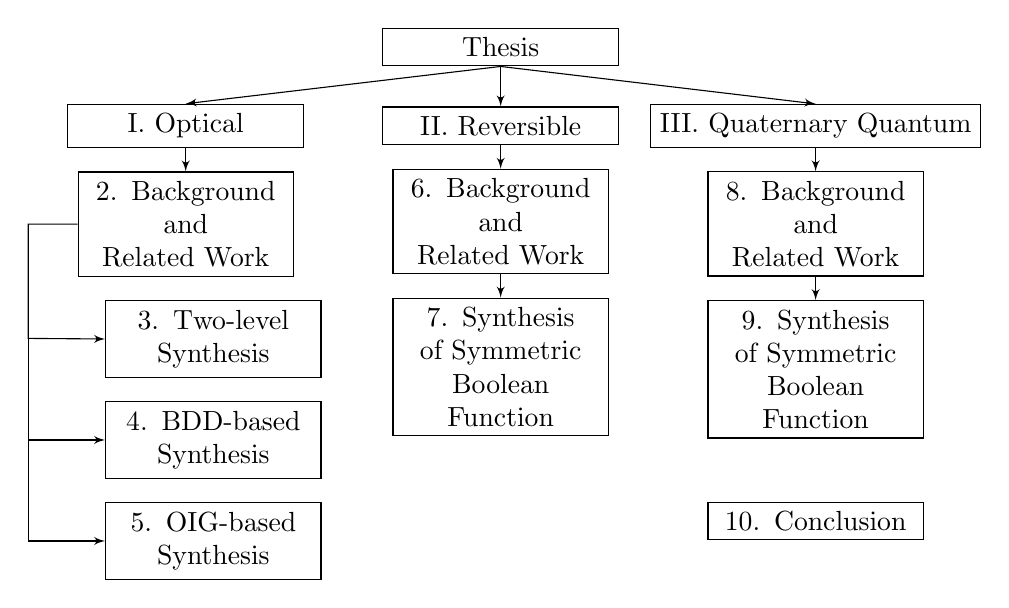
\begin{tikzpicture}
{
\pgftransformshift{\pgfpoint{0cm}{2cm}}
\pgfset{minimum width=3cm}
\pgfnode{rectangle}{center}{Thesis}{rec1}{\pgfusepath{stroke}}
}
{
\pgftransformshift{\pgfpoint{-4cm}{1cm}}
\pgfset{minimum width=3cm}
\pgfnode{rectangle}{center}{I. Optical}{rec2}{\pgfusepath{stroke}}
}
{
\pgftransformshift{\pgfpoint{0cm}{1cm}}
\pgfset{minimum width=3cm}
\pgfnode{rectangle}{center}{II. Reversible}{rec3}{\pgfusepath{stroke}}
}
{
\pgftransformshift{\pgfpoint{4cm}{1cm}}
\pgfset{minimum width=3cm}
\pgfnode{rectangle}{center}{III. Quaternary Quantum}{rec4}{\pgfusepath{stroke}}
}
\node[draw,rectangle,align=center, text width=2.5cm, below=3mm of rec2.south] (rec5) at (rec2.south) {2. Background \\ and \\ Related Work}; 
\node[draw,rectangle,align=center, text width=2.5cm, below=3mm of rec3.south] (rec6) at (rec3.south) {6. Background \\ and \\ Related Work}; 
\node[draw,rectangle,align=center, text width=2.5cm, below=3mm of rec4.south] (rec7) at (rec4.south) {8. Background \\ and \\ Related Work}; 
\node[draw,rectangle,align=center, text width=2.5cm, below=3mm of rec5.south, xshift=10] (rec8) at (rec5.south) {3. Two-level Synthesis}; 
\node[draw,rectangle,align=center, text width=2.5cm, below=3mm of rec8.south] (rec9) at (rec8.south) {4. BDD-based Synthesis}; 
\node[draw,rectangle,align=center, text width=2.5cm, below=3mm of rec9.south] (rec10) at (rec9.south) {5. OIG-based Synthesis}; 
\node[draw,rectangle,align=center, text width=2.5cm, below=3mm of rec6.south] (rec11) at (rec6.south) {7. Synthesis of Symmetric Boolean Function}; 
\node[draw,rectangle,align=center, text width=2.5cm, below=3mm of rec7.south] (rec12) at (rec7.south) {9. Synthesis of Symmetric Boolean Function}; 
\node[draw,rectangle,align=center, text width=2.5cm, below=8mm of rec12.south] (rec13) at (rec12.south) {10. Conclusion}; 

\pgfpointanchor{rec5}{west}
\pgfpointanchor{rec8}{west}

\coordinate (pt1) at (-6, -1.7);

\draw[draw, -latex'] (rec1.south) -- (rec2.north); 
\draw[draw, -latex'] (rec1.south) -- (rec3.north); 
\draw[draw, -latex'] (rec1.south) -- (rec4.north); 
\draw[draw, -latex'] (rec2.south) -- (rec5.north);
\draw[draw, -latex'] (rec3.south) -- (rec6.north);  
\draw[draw, -latex'] (rec4.south) -- (rec7.north);
\draw[draw, -latex'] (rec6.south) -- (rec11.north);  
\draw[draw, -latex'] (rec7.south) -- (rec12.north); 
\path[draw, -latex'] (rec5) -| (pt1) -- (rec8.west);
\path[draw, -latex'] (pt1) |- (rec9.west);
\draw[draw, -latex'] (pt1) |- (rec10.west);
\end{tikzpicture}
\caption{Structure of the thesis}
\label{fig:thesis-struct}
\end{figure}

%\section{Thesis Organization}

%%%%%%%%%%%%%%%%%%%%%%%%%%%%%%%%%%%%%%%%%%%%%%%%%%%%%%%%%%%%%%%%%%%%%%%%%%%%%%%%%%%%
\part{Optical Computing}
\chapter{Background on Optical Computing}

As discussed in the previous chapter, several technological realizations of optical circuits are currently considered. However, in order to ease the development of corresponding methods for the design automation of optical circuits, logic models, gate libraries, and cost metrics have been proposed which abstract from detailed physical and optical issues but discretely reflect the major constraints. To keep the thesis self-contained, this chapter provides a brief overview of optical gate libraries and cost metrics that are used in optical logic synthesis. The chapter is divided into two parts. In the first section, optical logic models and cost metrics are introduced. The next section presents a comprehensive literature survey related to optical logic synthesis.
  
\section{Optical Logic Models}

Optical devices allow to realize Boolean functions by means of optical switching elements, called as \emph{crossbar gates}, which route the optical
signals between two parallel paths. The inputs of both paths can either be
sourced by light (representing the logical value~``1'') or darkness (representing the logical value ``0''). Furthermore, the routing of both paths may be switched depending on the value of
an electrical signal. The output of each optical signal can be read using optical receivers. Logically, this leads to the following definition of a crossbar gate.

\begin{definition}
\label{def:crossbar}
A \emph{crossbar gate} realizes a Boolean 
function~$\B^3\rightarrow\B^2$ composed of two optical inputs~$p$ and~$q$, one 
electrical input~$x$, and two optical outputs~$f$ and~$g$. The signals~$p$ and~$q$
as well as~$f$ and~$g$ are connected by waveguides which, depending on the value of~$x$, realize either the identity
or a switch of the input values, i.e.~
$$\overline{x}\Rightarrow (p\equiv f) \wedge (q\equiv g) \mbox{\hspace{.5cm} and \hspace{.5cm}} x\Rightarrow (p\equiv g) \wedge (q\equiv f)$$
is realized. Fig.~\ref{fig:gates} provides the graphical representation of a crossbar gate.
\end{definition}

\def\centermove{0.8}
\begin{figure}
\centering
\subfloat[Gate]{\label{fig:gates_crossbar}~~~
\begin{tikzpicture}
\crossbarat{$x$}{0,0}{cb}
\node[crossin] at (cb.p) {$p$};
\node[crossin] at (cb.q) {$q$};
\node[crossout] at (cb.f) {$f$};
\node[crossout] at (cb.g) {$g$};
\node at (\centermove,0) {};
\node at (-\centermove,0) {};
\end{tikzpicture}~~~
}
\subfloat[Identity]{\label{fig:crossbar_identity}~~~
\begin{tikzpicture}
\functionalblockat{}{0,0}{cb}
\draw (cb.p) -- (cb.f);
\draw (cb.q) -- (cb.g);

\node[crossin] at (cb.p) {$p$};
\node[crossin] at (cb.q) {$q$};
\node[crossout] at (cb.f) {$f$};
\node[crossout] at (cb.g) {$g$};
\node at (\centermove,0) {};
\node at (-\centermove,0) {};
\node[draw=none, above=2.6mm of cb] (xbar) at (cb) {$\overline{x}$};
\end{tikzpicture}~~~
}
\subfloat[Switch]{\label{fig:crossbar_cross}~~~
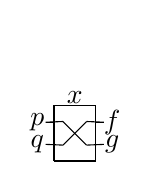
\begin{tikzpicture}
\functionalblockat{}{0,0}{cb}

\coordinate (pt1) at (-0.15,0.15) ; 
\coordinate (pt2) at (0.15,-0.15);
\coordinate (pt3) at (0.15,0.15);
\coordinate (pt4) at (-0.15,-0.15);

\draw (cb.p) -- (pt1);
\draw (cb.g) -- (pt2);
\draw (cb.f) -- (pt3);
\draw (cb.q) -- (pt4);
\draw (pt1) -- (pt2);
\draw (pt3) -- (pt4);

\node[draw=none, above=2.6mm of cb] (x) at (cb) {$x$};
\node[crossin] at (cb.p) {$p$};
\node[crossin] at (cb.q) {$q$};
\node[crossout] at (cb.f) {$f$};
\node[crossout] at (cb.g) {$g$};
\end{tikzpicture}~~~
}
\caption{Crossbar gate}\label{fig:gates}
\end{figure}

Note that, except for the crossbar gate, an optical signal cannot directly modify the value of an electrical signal and vice-versa. For such purposes, an opto-electrical interface would be required which, however, is considered as expensive as well as slow. Hence, electrical and optical signals are never assumed to interact with each other except for the crossbar gate. 

In addition to crossbar gates, splitters and combiners are also utilized as optical logic elements in order to realize logic functions.


\begin{definition}
% A \emph{splitter} divides an optical signal into two signals -- each with only half the signal
% power.
A \emph{splitter} divides an optical signal into two signals -- each with only half of the incoming
signal power.  In contrast, a \emph{combiner} merges two optical signals into a single one and, by
this, inherently realizes the OR-function. A splitter (combiner) may have more than two outputs
(inputs). Then, in case of a splitter, the strength of the signal is divided by the number of
outputs.
Fig.~\ref{fig:gates_splitter} and Fig.~\ref{fig:gates_combiner} provide the graphical representation of
both elements.
\end{definition}

Using these logic elements, a technology library is formed (as depicted in Fig.~\ref{fig:crossbar_gate_library}) that allows to realize arbitrary
Boolean functions.

\def\centermove{0.8}
\begin{figure}[!h]
\centering
\subfloat[Crossbar gate]{\label{fig:gates_crossbar_again}~~~
\begin{tikzpicture}
\crossbarat{$x$}{0,0}{cb}
\node[crossin] at (cb.p) {$p$};
\node[crossin] at (cb.q) {$q$};
\node[crossout] at (cb.f) {$f$};
\node[crossout] at (cb.g) {$g$};
\node at (\centermove,0) {};
\node at (-\centermove,0) {};
\end{tikzpicture}~~~
}
\subfloat[Splitter\label{fig:gates_splitter}]{
\begin{tikzpicture}
\node[splitter] {};
\node at (\centermove,0) {};
\node at (-\centermove,0) {};
\end{tikzpicture}
}
\subfloat[Combiner\label{fig:gates_combiner}]{
\begin{tikzpicture}
\node[combiner] {};
\node at (\centermove,0) {}; 
\node at (-\centermove,0) {};
\end{tikzpicture}
}
\caption{Optical gate library}\label{fig:crossbar_gate_library}
\end{figure}


\begin{figure}
\centering
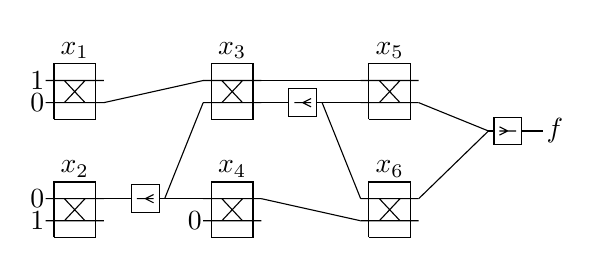
\begin{tikzpicture}
\crossbarat{$x_1$}{0,1.5}{a};
\crossbarat{$x_2$}{0,0}{b};

\crossbarat{$x_3$}{2,1.5}{c};
\crossbarat{$x_4$}{2,0}{d};

\crossbarat{$x_5$}{4,1.5}{e};
\crossbarat{$x_6$}{4,0}{f};

\node[splitter,xshift=15] (splitter) at (b.f) {};
\node[splitter,xshift=15] (splitter2) at (c.g) {};
\node[combiner] (combiner) at (5.5,1) {};
\node[xshift=10,inner sep=1] (fun) at (combiner.out) {$f$};

\draw (b.f) -- (splitter.in);
\draw (splitter.out) -- (d.p);
\draw (e.g) -- (combiner.in);
\draw (a.g) -- (c.p);
\draw (splitter.out) -- (c.q);
\draw (f.f) -- (combiner.in);
\draw (combiner.out) -- (fun);

\draw (c.f) -- (e.p);
\draw (c.g) -- (splitter2.in);
\draw (splitter2.out) -- (e.q);

\draw (splitter2.out) -- (f.p);

\draw (d.f) -- (f.q);

\node[crossin] at (a.p) {$1$};
\node[crossin] at (a.q) {$0$};

\node[crossin] at (b.p) {$0$};
\node[crossin] at (b.q) {$1$};

\node[crossin] at (d.q) {$0$};

\end{tikzpicture}
\caption{Optical circuit}
\label{fig:circuit}
\end{figure}


To measure the complexity of an optical circuit, several metrics got established in the literature~\cite{Condrat2011,WKHD:2015}. More precisely:
\begin{itemize}
\item The number of crossbar gates (often also denoted as gate costs): This metric is  motivated by the fact that each crossbar gate needs to be physically realized. Sometimes, also the number of splitter and the number of combiners are considered. However, as they are significantly easier to realize than the crossbar gates, they are often considered negligible. 

\item The worst case fraction: This metric is motivated by the fact that splitters in the circuit degrade the strength of the involved signal. Since simply counting the number of splitters provides an imprecise measure of the resulting effects (the impact of splitters will significantly differ if, e.g., ten splitters separately split ten signals or one signal ten times in a cascade), a more elaborate metric is considered. First, it is assumed that each splitter with $n$ outputs produces an output signal of strength $\nicefrac{1}{n}$. Then, the circuit's worst case fraction is determined by following all paths from the primary inputs to the primary outputs and multiplying all signal strengths produced by splitters visited on the current path. Afterwards, the maximum value of all paths is considered the worst case fraction\footnote{To keep the model simple, combiners are assumed not to change the signal strength. This makes the worst case fraction a pessimistic approximation i.e. the actual signal strength may be better than the computed one}.
\end{itemize}

\begin{example}
Fig.~\ref{fig:circuit} shows an optical circuit composed of six crossbar gates, two splitters, and
one combiner. The worst case fraction of the circuit is 4.
%The costs of the circuit depicted in Fig.~\ref{fig:circuit} are determined as
%6~crossbar gates, 2~splitters, 1~combiner, and
%a worst case fraction of~4.
\end{example}


Although these metrics are just approximations that may not perfectly correspond to the physical
implementation, it gives a better idea of the resulting circuit costs and signal strengths. 

In addition, an alternative gate library has also been used in the design and synthesis of optical circuits. According to alternative library, optical circuits are realized by means of a
\emph{Mach-Zehnder Interferometer}~(MZI) switch which is based on \emph{Semiconductor Optical Amplifiers}~(SOAs).
In the logic domain, the resulting structure is abstracted to a so-called \emph{MZI gate}.
Each MZI gate has two input ports and two output ports. The inputs can either be sourced by light (representing binary 1) or darkness (representing binary 0). Logically, an MZI gate is defined as follows~\cite{Scaffardi2008,QWang2004}:

\begin{definition}
An MZI gate realizes a Boolean function \mbox{$\B^2\rightarrow\B^2$} composed of two optical inputs~$p$ and~$q$ as well as two optical outputs~$f$ and~$g$. In the presence of both input signals, the outputs $f$ and $g$ produce $1$ and $0$, respectively. The presence of input signal $p$ and the absence of input signal $q$ leads to the logic value $0$ and $1$ at the outputs $f$ and~$g$, respectively. Therefore, the functions
$$f=p\wedge q \mbox{\hspace{.5cm} and \hspace{.5cm}} g=p\wedge q^{\prime}$$ 
are realized. Fig~\ref{fig:gates_crossbar} provides the graphical representation of an MZI gate.    
\end{definition} 

Like crossbar gate library, splitters and combiners are other optical logic elements in this library.

%\begin{definition}
%A \emph{splitter} divides an optical signal into two signals -- each with only half of the incoming
%signal power. In contrast, a \emph{combiner} merges two optical signals into a single one and, by
%this, inherently realizes the OR-function. A splitter (combiner) may have more than two outputs
%(inputs). Then, in case of a splitter, the strength of the signal is divided by the number of
%outputs.
%Fig.~\ref{fig:gates_splitter} and Fig.~\ref{fig:gates_combiner} provide the graphical representation %of
%both elements.
%\end{definition}

\def\centermove{0.8}
\begin{figure}[!h]
\centering
\subfloat[MZI gate\label{fig:gates_mzi}]{~~~
\begin{tikzpicture}
\functionalblockat{\tiny MZI}{0,0}{mzi}
\node[crossin] at (mzi.p) {$p$};
\node[crossin] at (mzi.q) {$q$};
\node[crossout] at (mzi.f) {$f$};
\node[crossout] at (mzi.g) {$g$};
\node at (\centermove,0) {};
\node at (-\centermove,0) {};
\end{tikzpicture}~~~
}
\subfloat[Splitter\label{fig:mzi_splitter}]{
\begin{tikzpicture}
\node[splitter] {};
\node at (\centermove,0) {};
\node at (-\centermove,0) {};
\end{tikzpicture}
}
\subfloat[Combiner\label{fig:mzi_combiner}]{
\begin{tikzpicture}
\node[combiner] {};
\node at (\centermove,0) {}; 
\node at (-\centermove,0) {};
\end{tikzpicture}
}
\vspace{-.1cm}
\caption{MZI gate library}\label{fig:mzi_gate_library}
\end{figure}

%Together these logic elements form a {\em gate library} that allows to realize any Boolean function.  

Although, the applied gate libraries are different, but the complexity of the optical circuits is measured based on the same cost metric i.e. number of gates (crossbar or MZI depending on the gate library) and worst case fraction. Additionally, it can be noted that the choice of any gate library particularly depends on the designers. 
 
%The size of an optical circuit is determined in terms of number of MZI gates. This is motivated by the fact that each MZI gate needs to be physically realized. Sometimes, also the number of splitters and the number of combiners are considered. However, as they are significantly easier to realize than the MZI gates, they are often considered negligible. % in size estimated metric. 
%Besides that, the number of splitters has an effect to the final strength of the applied optical signals.  

\begin{example}
Fig.~\ref{fig:circuit} shows an optical circuit composed of two MZI gates, two splitters, and one combiner. The worst case fraction of the circuit is 2.
\end{example}

\begin{figure}[!h]
\centering
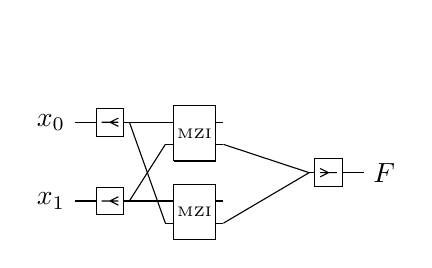
\begin{tikzpicture}
\functionalblockat{\tiny MZI}{0,0}{g2};
\functionalblockat{\tiny MZI}{0,1}{g1};
\node[shape=splittergate, xshift=-20] (s1) at (g1.p) {};
\node[shape=splittergate, xshift=-20] (s2) at (g2.p) {};
\node[shape=combinergate, xshift=20] (c1) at (1,0.5) {};
\node[left=2mm of s1.in] (a) {$\small x_0$};
\node[left=2mm of s2.in] (b) {$\small x_1$};
\node[right=2mm of c1.out] (F) {$\small F$};
 
\draw (a) -- (s1.in);
\draw (b) -- (s2.in); 
\draw (s1.out) -- (g1.p);
\draw (s1.out) -- (g2.q);
\draw (s2.out) -- (g1.q);
\draw (s2.out) -- (g2.p);
\draw (g1.g) -- (c1.in);
\draw (g2.g) -- (c1.in);
\draw (c1.out) -- (F); 
\end{tikzpicture}
\vspace{-.1cm}
\caption{Optical circuit}\vspace{-.5cm}
\label{fig:circuit}
\end{figure}

\section{Literature Review}

In mid 1980, the idea of making an all optical computer was conceived~\cite{TODO}. However, the CMOS technology was making steady progress during that time. Therefore, exploiting optics in computations was almost ignored. But in the last decades as CMOS technology is nearly ending, optical logic has re-emerged for computations. Several research works proposed and demonstrated basic Boolean operations~\cite{TODO}. In~\cite{Kim:06}, the authors have proposed all-optical multiple logic gates using two parallel semiconductor optical amplifier (SOA)-Mach-Zehnder interferometer (MZI) structures that enable simultaneous operations of various logic functions of XOR, NOR, OR, and NAND. The proposed scheme is experimentally demonstrated to confirm its validity. In~\cite{Nesset1995896,Houbavlis20041622,Kim2004608,dong200680gb}, an all-optical logic gate realizing AND operation are reported. All these realizations use different optical phenomena such as four-wave mixing~\cite{Nesset1995896}, cross phase modulation~\cite{Houbavlis20041622,Kim2004608} and semiconductor optical amplifier (SOA) based Mach-Zehnder interferometer (MZI)~\cite{dong200680gb}. In~\cite{kang2009all}, a method with high speed all-optical XOR and XNOR operations is proposed. While earlier realizations~\cite{Kim:06,dong200680gb} worked at 10 and 80 Gb/s, this works at 86.4 Gb/s. In~\cite{Martinez2007}, the authors proposed a Boolean device based on a single Mach-Zehnder interferometer with semiconductor optical amplifiers which can be reconfigured to operate as a logic XOR, AND, OR, and NOT gate. In~\cite{singh2012ultrahigh}, the author presented a design  of
all-optical  logic  gates  OR,  AND,  XNOR,  and  XOR  at  ultrahigh
speed. 

Besides logic gates, digital logic circuits received recent attention. Several combinational logic blocks such as adder~\cite{DattaCS15,cherri2010circuit,kumar2014implementation}, multiplexer~\cite{Datta2014}, divider~\cite{Aikawa2011} are proposed. In~\cite{kumar2014implementation}, the full adder and full subtractor are realized using an electro-optic Mach--Zehnder interferometers. In~\cite{cherri2010circuit}, the authors combine the attractive and powerful parallelism property of the modified signed-digit (MSD) number representation with the ultra-fast all-optical switching property of the semiconductor optical amplifier and Mach–Zehnder interferometer (SOA–MZI) to design and implement all-optical MSD adder/subtracter circuits. In~\cite{DattaCS15}, the authors proposed a ripple-carry adder, an extension with faster carry propagation, and a carry save adder. In~\cite{}, the authors proposed directed logic, where different logic circuits with two logical outputs; one
complements the other. Additionally, a programmable logic unit has been proposed~\cite{Chattopadhyay:11}. This realization is limited to 2 inputs only.

However, all these are ad hoc solutions in the sense that each of them 
\begin{itemize}
\item has mainly been derived manually for a special purpose,
\item addresses a very specific type of functional block, 
\item is often not extendable to arbitrary functions, and
\item is typically suitable for small functions only, i.e.~is limited 
with respect to its scalability. %, with the scalability properties being very limited.
\end{itemize}
A first attempt towards generic approaches has been considered in~\cite{Condrat2011}. Here, synthesis approach based on BDD is proposed. This enables synthesis of functions containing over 100 variables and thus is a major step towards design of complex systems in optical logic. Recently, another BDD based approach is reported in~\cite{TODO}. While, optical circuit composed of crossbar gates are obtained from~\cite{Condrat2011}, solution proposed in~\cite{TODO} generates circuits composed of MZI gates. Although, these solutions synthesized circuits using two different gate libraries, they have a common shortcoming. Both designs, irrespective of gate library generates circuits consisting of huge number of splitters which ultimately leads to poor signal strength. To avoid this problem, an alternative solution again based on BDD is proposed in~\cite{TODO}. This scheme generates splitter-free circuit.  

%%%%%%%%%%%%%%%%%%%%%%%%%%%%%%%%%%%%%%%%%%%%%%%%%%%%%%%%%%%%%%%%%%%%%%%%%%%%%%%%%%%%%

\chapter{Synthesis of Optical Circuit Using Two-Level Representations}~\label{ch:synth-two-level}
\chaptermark{Two-Level synthesis}

\section{Two-Level Representation}
Besides BDDs, also so-called two level function descriptions such as
\emph{Sum of Products}~(SOP) or \emph{Exclusive Sum of Products}~(ESOP)
are established means which also allow for the efficient representation
of large Boolean functions.
An SOP represents a Boolean function in terms of 
a disjunction~(OR) of conjunctions (AND) of literals.
A \emph{literal} is either a propositional variable or its negation.
That is, an SOP is an AND-OR expression.
The conjunction of literals is usually called a \emph{product} or a \emph{cube}
and is denoted by~$C$ in the following.
Vice versa, an ESOP represents a Boolean function in terms of 
exclusive disjunction~(XOR) of products and, hence, is an AND-XOR expression.
%\subsection{Sum-of-Products}
\todo[inline]{write like definition}
\begin{example}
We illustrate both two level function representations by the functions~$f$ and~$h$ which are represented by the
\begin{itemize}
\item SOP as shown in Fig.~\subref*{fig:function_sop} and
\item ESOP as shown in Fig.~\subref*{fig:function_esop}, respectively.
\end{itemize}
More precisely, the column on the left-hand side shows the respective products, where a~``$1$'' on
the $i^{\rm th}$ position denotes a positive literal (i.e.~$x_i$) and a~``$0$'' denotes a negative
literal (i.e.~$\overline{x}_i$), respectively.
A ``--'' denotes that the respective variable is not included in the product.
The right-hand side gives the respective primary output patterns to which the OR or XOR is applied.
\end{example}

%\subsection{Exclusive-Sum-of-Products}
\todo[inline]{write like definition}
\begin{example}
Add example
\end{example}

\section{Gate-Efficient Synthesis}
Since both, SoP and ESoP, rely on the realization of the respective products, therefore, first synthesis of the conjunction of literals is described. Afterwards, how to realize the disjunction or exclusive disjunction of the resulting structures is described, respectively.

\subsection{Realization of Product Terms}
Without loss of generality, 
consider a product \mbox{$C_{i}=x_{i_{1}}x_{i_{2}}x_{i_{3}}\cdots x_{i_{k}}$} composed of positive
literals only.
%where, each $x_{i_{j}}$ is a positive literal. 
Such a product can be realized by an optical circuit of crossbar gates as shown in 
Fig.~\subref*{fig:positive-literal-one}. 
For each literal~$x_{i_{j}}\in C_{i}$,
a crossbar gate is added. The respective inputs/outputs are connected in a fashion
so that the input value~$1$ at the first crossbar gate of the circuit in Fig.~\subref*{fig:positive-literal-one} is passed through all gates to the output~$C_{i}$ iff all literals are indeed assigned~$1$. In order to additionally support negative literals, the respective signal connections have to
be flipped as illustrated in Fig.~\subref*{fig:internal2} for a product 
$C_{i}=x_{i_{1}}\overline{x}_{i_{2}}x_{i_{3}}\cdots x_{i_{k}}$
with a negative literal~$\overline{x}_{i_{2}}$.

Alternatively, the products can also be realized by the optical circuits of crossbar gates as shown in   Fig.~\subref*{fig:internal} and Fig.~\subref*{fig:internal2} with positive and mixed literals, respectively. Here, the inputs/outputs of crossbar gates are connected in such a manner so that the input value-$1$ at the bottom of the circuit and input value-$0$ at the top of the circuit in Fig.~\subref*{fig:internal} are passed through all gates to the outputs~$C_{i}$ and $\overline{C_{i}}$, respectively iff all literals are indeed assigned~$1$. This type of circuit allows realization of the product and its complement i.e. AND-NAND realization at the same time.
Note that, both forms of the circuit require the same amount of crossbar gates as each crossbar gate corresponds a literal in the product. In the following, both forms of realization for a product~\mbox{$x_{i_{j}}\in C_{i}$} are represented by the functional blocks as depicted in Fig.~\subref*{fig:functional-block-one} and~\subref*{fig:functional-block-two}. In case of Fig.~\subref*{fig:functional-block-one}, the set $\{0,0,\cdots,0\}$ denotes the value-$0$ applied at the input of each crossbar gate as depicted in Fig.~\subref*{fig:positive-literal-one} and~\subref*{fig:mixed-literal-one}.  

\begin{figure}[!h]
\centering
\subfloat[Positive literals only\label{fig:positive-literal-one}]{
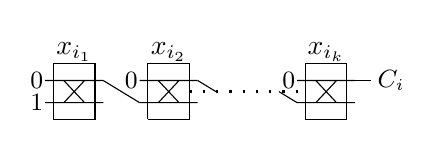
\begin{tikzpicture}
\crossbarat{$x_{i_{1}}$}{0,0}{x1}
\crossbarat{$x_{i_{2}}$}{1.2,0}{x2}
\crossbarat{$x_{i_{k}}$}{3.2,0}{xk}

\node[xshift=1em,outer sep=1pt] (f1) at (xk.f) {};
\coordinate (pt1) at (1.8,0);
\coordinate (pt2) at (2.6,0);

\draw (x1.f) -- (x2.q);
\draw (x2.f) -- (pt1);
\draw (xk.q) -- (pt2);

\draw[xshift=20,loosely dotted,thick] (x2) -- (xk);
\draw (xk.f) -- (f1);

\node[crossin] at (x1.p) {\small $0$};
\node[crossin] at (x1.q) {\small $1$};
\node[crossin] at (x2.p) {\small $0$};
\node[crossin] at (xk.p) {\small $0$};
\node[crossout] at (f1) {\small $C_{i}$};
\end{tikzpicture}}%~~~~~~~~~~~~~~~~~~~~~~~~~~~~
~~~
\subfloat[Mixed literals\label{fig:mixed-literal-one}]{
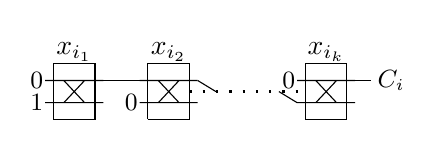
\begin{tikzpicture}
\crossbarat{$x_{i_{1}}$}{0,0}{x1}
\crossbarat{$x_{i_{2}}$}{1.2,0}{x2}
\crossbarat{$x_{i_{k}}$}{3.2,0}{xk}

\node[xshift=1em,outer sep=1pt] (f1) at (xk.f) {};
\coordinate (pt1) at (1.8,0);
\coordinate (pt2) at (2.6,0);

\draw (x1.f) -- (x2.p);
\draw (x2.f) -- (pt1);
\draw (xk.q) -- (pt2);

\draw[xshift=20,loosely dotted,thick] (x2) -- (xk);
\draw (xk.f) -- (f1);

\node[crossin] at (x1.p) {\small $0$};
\node[crossin] at (x1.q) {\small $1$};
\node[crossin] at (x2.q) {\small $0$};
\node[crossin] at (xk.p) {\small $0$};
\node[crossout] at (f1) {\small $C_{i}$};
\end{tikzpicture}}%~~~~~~~~~~~~~~
~~~
\subfloat[Functional block\label{fig:functional-block-one}]{
\begin{tikzpicture}
%\node at (0,-.1) {};
%\node at (2,0) {};

\functionalblockat{\small $C_i$} {0,0} {C1}

\node[xshift=7] (C1p) at (C1.p) {};
\node[left =of C1p,xshift=20] (C1pp) {\small $\{0,0,\cdots,0\}$};
\node[xshift=7] (C1q) at (C1.q) {};
\node[left =of C1q,xshift=20] (C1qq) {\small $1$};
\node[xshift=-7] (C1f) at (C1.f) {};
\node[right =of C1f,xshift=-15] (C1ff) {\small $C_{i}$};
\node[xshift=-7] (C1g) at (C1.g) {};
%\node[right =of C1g,xshift=-15] (C1gg) {\small $\overline{C}_{i}$};

\draw (C1p) -- (C1.p);
\draw (C1pp) -- (C1.p);
\draw (C1q) -- (C1.q);
\draw (C1qq) -- (C1.q);
\draw (C1f) -- (C1.f);
\draw (C1ff) -- (C1.f);
\draw (C1g) -- (C1.g);
%\draw (C1gg) -- (C1.g);

%\node (r1) at (0,0) {};

%\node[right=of r1, draw=none, xshift=20,inner sep=0] (r2) {};
%\node[above=of r2, draw=none, yshift=18,inner sep=0] (r3) {};
%\node[above=of r1, draw=none, xshift=3,yshift=15,inner sep=0] (r4) {}; 

%\draw (r1.east) -- (r2.east);
%\draw (r2.east) -- (r3.east);
%\draw (r3.east) -- (r4.east);
%\draw (r4.east) -- (r1.east);

%\node[above =of r1, draw=none,xshift=3,yshift=5,inner sep=0] (r5) {};
%\node[left =of r5, draw=none,inner sep=0] (r6) {$p$};

%\draw (r5.east) -- (r6.east);

%\node[below =of r4, draw=none,yshift=-8,inner sep=0] (r7) {};
%\node[left =of r7, draw=none,inner sep=0] (r8) {$q$};

%\draw (r7.east) -- (r8.east);

%\node[above =of r2, draw=none,yshift=7,inner sep=0] (r9) {};
%\node[right =of r9, draw=none,inner sep=1] (r10) {$f$};

%\draw (r9.east) -- (r10.west);

%\node[below =of r3, draw=none,yshift=-8,inner sep=0] (r11) {};
%\node[right =of r11, draw=none,inner sep=0] (r12) {$g$};

%\draw (r11.east) -- (r12.west);

%\node[midway, above right=of r4, draw=none,xshift=-5,yshift=20,inner sep=0] (r13) %{$C_i$};

\end{tikzpicture}}
\caption{Realization of product terms}
\end{figure}

\begin{figure}[!h]
\centering
\subfloat[Positive literals only\label{fig:internal}]{\hspace{1cm}
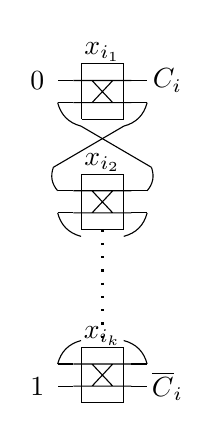
\begin{tikzpicture}
\crossbarat{$x_{i_{1}}$}{0,2.2}{x1}
\crossbarat{$x_{i_{2}}$}{0,0.8}{x2}
%\crossbarat{$x_3$}{0,.2}{x3}
\crossbarat{$x_{i_{k}}$}{0,-1.4}{xk}

\node[xshift=-1em,outer sep=1pt] (p1) at (x1.p) {};
\node[xshift=-1em,outer sep=1pt] (q1) at (x1.q) {};
\node[xshift=1em,outer sep=1pt] (f1) at (x1.f) {};
\node[xshift=-1em,outer sep=1pt] (p2) at (x2.p) {};
\node[xshift=1em,outer sep=1pt] (g1) at (x1.g) {};
\node[xshift=1em,outer sep=1pt] (f2) at (x2.f) {};
\node[xshift=-1em,outer sep=1pt] (q2) at (x2.q) {};
\node[xshift=1em,outer sep=1pt] (g2) at (x2.g) {};
%\node[xshift=-1em,outer sep=1pt] (p3) at (x3.p) {};
%\node[xshift=-1em,outer sep=1pt] (q3) at (x3.q) {};
%\node[xshift=1em,outer sep=1pt] (f3) at (x3.f) {};
%\node[xshift=1em,outer sep=1pt] (g3) at (x3.g) {};
\node[xshift=-1em,outer sep=1pt] (pk) at (xk.p) {};
\node[xshift=-1em,outer sep=1pt] (qk) at (xk.q) {};
\node[xshift=1em,outer sep=1pt] (fk) at (xk.f) {};
\node[xshift=1em,outer sep=1pt] (gk) at (xk.g) {};

\draw (x1.p) -- (p1);
\draw (x1.q) -- (q1);
\draw (x1.f) -- (f1);
\draw (x2.p) -- (p2);
\draw (x1.g) -- (g1);
\draw (x2.f) -- (f2);
\draw (x2.q) -- (q2);
\draw (x2.g) -- (g2);
%\draw (x3.p) -- (p3);
%\draw (x3.q) -- (q3);
%\draw (x3.f) -- (f3);
%\draw (x3.g) -- (g3);
\draw (xk.p) -- (pk);
\draw (xk.q) -- (qk);
\draw (xk.f) -- (fk);
\draw (xk.g) -- (gk);


\node[below right=of q1, draw=none,xshift=-20,yshift=25,inner sep=0] (q11) {};
\node[below left=of g1, draw=none,xshift=20,yshift=25,inner sep=0] (g11) {};

\draw[bend right] (q1.east) to node [auto] {} (q11.west);
\draw[bend left] (g1.west) to node [auto] {} (g11.east);

\node[above right=of p2, draw=none,xshift=-30,yshift=-25,inner sep=0] (p22) {};
\node[above left=of f2, draw=none,xshift=30,yshift=-25,inner sep=0] (f22) {};

\draw[bend left] (p2.east) to node [auto] {} (p22.west);
\draw[bend right] (f2.west) to node [auto] {} (f22.east);

\draw (q11.west) -- (f22.east);
\draw (p22.west) -- (g11.east);

\node[below right=of q2, draw=none,xshift=-20,yshift=25,inner sep=0] (q22) {};
\node[below left=of g2, draw=none,xshift=20,yshift=25,inner sep=0] (g22) {};

\draw[bend right] (q2.east) to node [auto] {} (q22.west);
\draw[bend left] (g2.west) to node [auto] {} (g22.east);

%\node[above right=of p3, draw=none,xshift=-20,yshift=-25,inner sep=0] (p33) {};
%\node[above left=of f3, draw=none,xshift=20,yshift=-25,inner sep=0] (f33) {};

%\draw[bend left] (p3.east) to node [auto] {} (p33.west);
%\draw[bend right] (f3.west) to node [auto] {} (f33.east);

%\draw (q22.west) -- (f33.east);
%\draw (p33.west) -- (g22.east);

%\node[below right=of q3, draw=none,xshift=-20,yshift=25,inner sep=0] (q33) {};
%\node[below left=of g3, draw=none,xshift=20,yshift=25,inner sep=0] (g33) {};

%\draw[bend right] (q3.east) to node [auto] {} (q33.west);
%\draw[bend left] (g3.west) to node [auto] {} (g33.east);

%\node[below =of q33, draw=none,yshift=25,inner sep=0] (p44) {};
%\node[below =of g33, draw=none,yshift=25,inner sep=0] (f44) {};

%\draw (q33.west) -- (f44.west);
%\draw (g33.east) -- (p44.east);

\node[above right=of pk, draw=none,xshift=-20,yshift=-25,inner sep=0] (pkk) {};
\node[above left=of fk, draw=none,xshift=20,yshift=-25,inner sep=0] (fkk) {};

\draw[bend left] (pk.east) to node [auto] {} (pkk.west);
\draw[bend right] (fk.west) to node [auto] {} (fkk.east);

\node[above =of pkk, draw=none,yshift=-25,inner sep=0] (pl) {};
\node[above =of fkk, draw=none,yshift=-25,inner sep=0] (fl) {};

%\draw (pkk.west) -- (fl.west);
%\draw (fkk.east) -- (pl.east);

\draw[xshift=20,loosely dotted,thick] (x2) -- (xk);

\node[crossin] at (p1) {$0$};
\node[crossin] at (qk) {$1$};
\node[crossout] at (f1) {$C_{i}$};
\node[crossout] at (gk) {$\overline{C}_{i}$};
\end{tikzpicture}}%~~~~~~~~~~~~~~~~~~~~~~~~~~~~
~~~
\subfloat[Mixed literals\label{fig:internal2}]{\hspace{1cm}
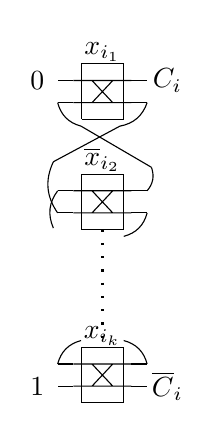
\begin{tikzpicture}
\crossbarat{$x_{i_{1}}$}{0,2.2}{x1}
\crossbarat{$\overline{x}_{i_{2}}$}{0,0.8}{x2}
%\crossbarat{$x_3$}{0,.2}{x3}
\crossbarat{$x_{i_{k}}$}{0,-1.4}{xk}

\node[xshift=-1em,outer sep=1pt] (p1) at (x1.p) {};
\node[xshift=-1em,outer sep=1pt] (q1) at (x1.q) {};
\node[xshift=1em,outer sep=1pt] (f1) at (x1.f) {};
\node[xshift=-1em,outer sep=1pt] (p2) at (x2.p) {};
\node[xshift=1em,outer sep=1pt] (g1) at (x1.g) {};
\node[xshift=1em,outer sep=1pt] (f2) at (x2.f) {};
\node[xshift=-1em,outer sep=1pt] (q2) at (x2.q) {};
\node[xshift=1em,outer sep=1pt] (g2) at (x2.g) {};
%\node[xshift=-1em,outer sep=1pt] (p3) at (x3.p) {};
%\node[xshift=-1em,outer sep=1pt] (q3) at (x3.q) {};
%\node[xshift=1em,outer sep=1pt] (f3) at (x3.f) {};
%\node[xshift=1em,outer sep=1pt] (g3) at (x3.g) {};
\node[xshift=-1em,outer sep=1pt] (pk) at (xk.p) {};
\node[xshift=-1em,outer sep=1pt] (qk) at (xk.q) {};
\node[xshift=1em,outer sep=1pt] (fk) at (xk.f) {};
\node[xshift=1em,outer sep=1pt] (gk) at (xk.g) {};

\draw (x1.p) -- (p1);
\draw (x1.q) -- (q1);
\draw (x1.f) -- (f1);
\draw (x2.p) -- (p2);
\draw (x1.g) -- (g1);
\draw (x2.f) -- (f2);
\draw (x2.q) -- (q2);
\draw (x2.g) -- (g2);
%\draw (x3.p) -- (p3);
%\draw (x3.q) -- (q3);
%\draw (x3.f) -- (f3);
%\draw (x3.g) -- (g3);
\draw (xk.p) -- (pk);
\draw (xk.q) -- (qk);
\draw (xk.f) -- (fk);
\draw (xk.g) -- (gk);


\node[below right=of q1, draw=none,xshift=-20,yshift=25,inner sep=0] (q11) {};
\node[below left=of g1, draw=none,xshift=20,yshift=25,inner sep=0] (g11) {};

\draw[bend right] (q1.east) to node [auto] {} (q11.west);
\draw[bend left] (g1.west) to node [auto] {} (g11.west);

\node[above right=of q2, draw=none,xshift=-30,yshift=-15,inner sep=0] (q22) {};
%\node[above right=of p2, draw=none,xshift=-20,yshift=-25,inner sep=0] (p22) {};
\node[above left=of f2, draw=none,xshift=30,yshift=-25,inner sep=0] (f22) {};

\draw[bend left] (q2.east) to node [auto] {} (q22.west);
%\draw[bend left] (p2.east) to node [auto] {} (p22.west);
\draw[bend right] (f2.west) to node [auto] {} (f22.east);

\draw (q11.west) -- (f22.east);
\draw (q22.west) -- (g11.west);

\node[below right=of p2, draw=none,xshift=-30,yshift=20,inner sep=0] (p22) {};
%\node[below right=of q2, draw=none,xshift=-20,yshift=25,inner sep=0] (q22) {};
\node[below left=of g2, draw=none,xshift=20,yshift=25,inner sep=0] (g22) {};

\draw[bend right] (p2.east) to node [auto] {} (p22.west);
%\draw[bend right] (q2.east) to node [auto] {} (q22.west);
\draw[bend left] (g2.west) to node [auto] {} (g22.east);

%\node[above right=of p3, draw=none,xshift=-20,yshift=-25,inner sep=0] (p33) {};
%\node[above left=of f3, draw=none,xshift=20,yshift=-25,inner sep=0] (f33) {};

%\draw[bend left] (p3.east) to node [auto] {} (p33.west);
%\draw[bend right] (f3.west) to node [auto] {} (f33.east);

%\draw (q22.west) -- (f33.east);
%\draw (p33.west) -- (g22.east);

%\node[below right=of q3, draw=none,xshift=-20,yshift=25,inner sep=0] (q33) {};
%\node[below left=of g3, draw=none,xshift=20,yshift=25,inner sep=0] (g33) {};

%\draw[bend right] (q3.east) to node [auto] {} (q33.west);
%\draw[bend left] (g3.west) to node [auto] {} (g33.east);

%\node[below =of q33, draw=none,yshift=25,inner sep=0] (p44) {};
%\node[below =of g33, draw=none,yshift=25,inner sep=0] (f44) {};

%\draw (q33.west) -- (f44.west);
%\draw (g33.east) -- (p44.east);

\node[above right=of pk, draw=none,xshift=-20,yshift=-25,inner sep=0] (pkk) {};
\node[above left=of fk, draw=none,xshift=20,yshift=-25,inner sep=0] (fkk) {};

\draw[bend left] (pk.east) to node [auto] {} (pkk.west);
\draw[bend right] (fk.west) to node [auto] {} (fkk.east);

\node[above =of pkk, draw=none,yshift=-25,inner sep=0] (pl) {};
\node[above =of fkk, draw=none,yshift=-25,inner sep=0] (fl) {};

%\draw (pkk.west) -- (fl.west);
%\draw (fkk.east) -- (pl.east);

\draw[xshift=20,loosely dotted,thick] (x2) -- (xk);

\node[crossin] at (p1) {$0$};
\node[crossin] at (qk) {$1$};
\node[crossout] at (f1) {$C_{i}$};
\node[crossout] at (gk) {$\overline{C}_{i}$};
\end{tikzpicture}}%~~~~~~~~~~~~~~
~~~
\subfloat[Functional block\label{fig:functional-block-two}]{
	\centering
\begin{tikzpicture}


\node at (0,-.1) {};
\node at (2,0) {};

\functionalblockat{\small $C_i$} {0,2} {C1}

\node[xshift=7] (C1p) at (C1.p) {};
\node[left =of C1p,xshift=20] (C1pp) {\small $0$};
\node[xshift=7] (C1q) at (C1.q) {};
\node[left =of C1q,xshift=20] (C1qq) {\small $1$};
\node[xshift=-7] (C1f) at (C1.f) {};
\node[right =of C1f,xshift=-15] (C1ff) {\small $C_{i}$};
\node[xshift=-7] (C1g) at (C1.g) {};
\node[right =of C1g,xshift=-15] (C1gg) {\small $\overline{C}_{i}$};

\draw (C1p) -- (C1.p);
\draw (C1pp) -- (C1.p);
\draw (C1q) -- (C1.q);
\draw (C1qq) -- (C1.q);
\draw (C1f) -- (C1.f);
\draw (C1ff) -- (C1.f);
\draw (C1g) -- (C1.g);
\draw (C1gg) -- (C1.g);

%\node (r1) at (0,0) {};

%\node[right=of r1, draw=none, xshift=20,inner sep=0] (r2) {};
%\node[above=of r2, draw=none, yshift=18,inner sep=0] (r3) {};
%\node[above=of r1, draw=none, xshift=3,yshift=15,inner sep=0] (r4) {}; 

%\draw (r1.east) -- (r2.east);
%\draw (r2.east) -- (r3.east);
%\draw (r3.east) -- (r4.east);
%\draw (r4.east) -- (r1.east);

%\node[above =of r1, draw=none,xshift=3,yshift=5,inner sep=0] (r5) {};
%\node[left =of r5, draw=none,inner sep=0] (r6) {$p$};

%\draw (r5.east) -- (r6.east);

%\node[below =of r4, draw=none,yshift=-8,inner sep=0] (r7) {};
%\node[left =of r7, draw=none,inner sep=0] (r8) {$q$};

%\draw (r7.east) -- (r8.east);

%\node[above =of r2, draw=none,yshift=7,inner sep=0] (r9) {};
%\node[right =of r9, draw=none,inner sep=1] (r10) {$f$};

%\draw (r9.east) -- (r10.west);

%\node[below =of r3, draw=none,yshift=-8,inner sep=0] (r11) {};
%\node[right =of r11, draw=none,inner sep=0] (r12) {$g$};

%\draw (r11.east) -- (r12.west);

%\node[midway, above right=of r4, draw=none,xshift=-5,yshift=20,inner sep=0] (r13) %{$C_i$};
\end{tikzpicture}}
\caption{Alternative realization of product terms}
\end{figure}

\subsection{Synthesis based on SoP Representation}
Having the building blocks of all product terms $C_{i}$ of an SoP~$f=C_1 \vee \dots \vee C_d$,
the entire function can be realized by adding logic which ORs the output signals of all those blocks.
Since the OR-operation is inherently realized by a combiner, this can easily be conducted.
However, for SoPs representing multiple-output functions~$f:\mathbb{B}^{n}\rightarrow\mathbb{B}^{m}$,
products might be required more than once. Then, a splitter is added to make the intermediate results at the outputs of the building blocks available to all functions relying on it. 
The following example illustrates the idea.

\begin{example}
Consider again the SoP
%multiple-output function~$f:\mathbb{B}^{n}\rightarrow\mathbb{B}^{m}$
shown in Fig.~\subref*{fig:function_sop}.
Fig.~\subref*{fig:sopcircuit} shows the optical circuit obtained from this SOP.
The building blocks denoted $C_1, C_2, C_3$ realize the corresponding products from the left-hand side of Fig.~\subref*{fig:function_sop}.
Since the first product $C_1$ belongs to both outputs, a splitter is added 
to derive two copies of the signal value~$C_1$. 
Afterwards, combiners merge the optical signals in order to realize the disjunction
of~$C_1$ and~$C_2$ (realizing~$f_1$) and of~$C_1$ and~$C_3$ (realizing~$f_2$).
\end{example} 

The above SoP scheme shares the common product terms among multiple output functions, however, the product terms frequently contain common set of literals leading to redundant computations of the respective factors. The common set of literals enables the possibility of sharing which allows a significant reduction in number of crossbar gates.

The general idea is as follows: \todo[inline]{The above discussion shows a straightforward mapping of SoP representation to optical circuits. Although the common product terms are shared among outputs, however, the common literals among product terms are not considered. Therefore, considering common literals would lead to better circuit realization with respect to number of crossbar gates. In the following, the general idea of common literal reduction is presented. Here, use the text from add line/common control reduction paper.}



\subsection{Synthesis based on ESoP Representation}

\newpage

\section{Splitter-Free Synthesis}

\newpage

\subsection{Synthesis based on SoP Representation}

\newpage

\subsection{Synthesis based on ESoP Representation}

\newpage

\section{Post-Synthesis Optimization Method}

\newpage

\section{Experimental Evaluation}

\newpage

\section{Discussion}

\newpage

\section{Chapter Contribution and Summary}
\newpage

%%%%%%%%%%%%%%%%%%%%%%%%%%%%%%%%%%%%%%%%%%%%%%%%%%%%%%%%%%%%%%%%%%%%%%%%%%%%%%%%%%%%%
\chapter{Synthesis of Optical Circuit Using Binary Decision Diagram}~\label{ch:opt-circ-bdd}
\chaptermark{BDD-based synthesis}
As mentioned earlier, synthesis is the most important step in designing complex digital circuit.
The initial work on logic synthesis of optical circuits was primarily involved in realizing basic Boolean operations~\cite{Kim:06,Martinez2007,Taraphdar2010}. Later, some important arithmetic units such as adder~\cite{DattaCS15}, multiplexer~\cite{Datta2014}, divider~\cite{Aikawa2011} have been realized in optical domain. Although, this shows a progress in the development of optical logic circuits, the designs are limited to single applications only. Therefore, synthesis approaches are required to efficiently generate any Boolean function -- an initial step towards design automation.

The desired behavior of the circuit to be synthesized is given by function descriptions like \emph{Binary Decision Diagrams}~(BDDs), two-level descriptions including \emph{Sum-of-Products}~(SoPs) and \emph{Exclusive-Sum-of-Products}~(ESoPs). Thus far, a particular consideration has been put on synthesis using \emph{Binary Decision Diagrams}~(BDDs)~\cite{Condrat2011,WKHD:2015}. BDDs are a data-structure for the efficient representation of large Boolean functions~\cite{Bryant1986} and allow for scalable circuit synthesis. Consequently, two approaches for the synthesis of optical circuits based on BDDs have been proposed: one employs a direct mapping scheme~\cite{Condrat2011}, where each node of the BDD is substituted by an optical gate. Furthermore, the sharing of a node is realized by a splitter which divides the optical signal into many. As this causes huge fractions of signal strength, an alternative has been proposed in~\cite{WKHD:2015} employing a reverse scheme avoiding splitting of signals and, hence, signal fractions at all (both approaches are later reviewed in more detail in Section~\ref{sec:bdd-synthesis}). 

Recent advances in the physical realization of optical devices~\cite{TODO} further motivated the consideration of several technological realizations of optical circuits. 
To develop automatic synthesis approaches for realization of optical circuits, corresponding logic models, gate libraries, and cost metrics have been proposed which abstract from detailed physical and optical issues but discretely reflect the major constraints.  
Section~\ref{sec:optical-logic-model} briefly reviews the optical logic gates and cost metrics as well as \emph{Binary Decision Diagrams}~(BDDs). In Section~\ref{sec:bdd-synthesis}, both BDD-based synthesis approaches are briefly reviewed. 
Section~\ref{sec:motivation-for-bdd-opt} discusses the downside of the existing approaches and introduces the general idea of exploiting BDD optimization in synthesis of optical circuits. To this end, the core idea of BDD optimization technique is provided in Section~\ref{sec:bdd-minimization}. Section~\ref{sec:bdd-min-results} demonstrates the effect of these optimization techniques on the resulting circuits through experimentally evaluation, while Section~\ref{sec:bdd-summary} summarizes the contribution of the chapter. 

%\section{Preliminaries}~\label{sec:prelim-bdd}
%\subsection{Applied Circuit Model and Cost Metric}~\label{sec:optical-logic-model}

In this abstraction, Boolean functions can be realized by optical switching elements, called as \emph{crossbar gates}, which route the optical
signals between two parallel paths. The inputs of both paths can either be
sourced by light (representing the logical value~``1'') or darkness (representing the logical value ``0'').
Furthermore, the routing of both paths may be switched depending on the value of
an electrical signal.
The output of each optical signal can be read using optical receivers. Logically, this leads to the following definition of a crossbar gate.

\begin{definition}
\label{def:crossbar}
A \emph{crossbar gate} realizes a Boolean 
function~$\B^3\rightarrow\B^2$ composed of two optical inputs~$p$ and~$q$, one 
electrical input~$x$, and two optical outputs~$f$ and~$g$. The signals~$p$ and~$q$
as well as~$f$ and~$g$ are connected by waveguides which, depending on the value of~$x$, realize either the identity
or a switch of the input values, i.e.~
$$\overline{x}\Rightarrow (p\equiv f) \wedge (q\equiv g) \mbox{\hspace{.5cm} and \hspace{.5cm}} x\Rightarrow (p\equiv g) \wedge (q\equiv f)$$
is realized. Fig.~\subref*{fig:gates_crossbar} provides the graphical representation of a crossbar gate.
\end{definition}

\def\centermove{0.8}
\begin{figure}
\centering
\subfloat[Crossbar gate]{\label{fig:gates_crossbar}~~~
\begin{tikzpicture}
\crossbarat{$x$}{0,0}{cb}
\node[crossin] at (cb.p) {$p$};
\node[crossin] at (cb.q) {$q$};
\node[crossout] at (cb.f) {$f$};
\node[crossout] at (cb.g) {$g$};
\node at (\centermove,0) {};
\node at (-\centermove,0) {};
\end{tikzpicture}~~~
}
\subfloat[Splitter\label{fig:gates_splitter}]{
\begin{tikzpicture}
\node[splitter] {};
\node at (\centermove,0) {};
\node at (-\centermove,0) {};
\end{tikzpicture}
}
\subfloat[Combiner\label{fig:gates_combiner}]{
\begin{tikzpicture}
\node[combiner] {};
\node at (\centermove,0) {}; 
\node at (-\centermove,0) {};
\end{tikzpicture}
}
\caption{Optical gates}\label{fig:gates}
\end{figure}

Note that, except for the crossbar gate as defined above, an optical signal cannot directly modify the value of an electrical signal and vice-versa. For such purposes, an opto-electrical interface would be required which, however, is considered as expensive as well as slow. Hence, electrical and optical signals are never assumed to interact with each other except for the crossbar gate. 


In addition to crossbar gates, splitters and combiners are also utilized as optical logic elements in order to realize logic functions.


\begin{definition}
% A \emph{splitter} divides an optical signal into two signals -- each with only half the signal
% power.
A \emph{splitter} divides an optical signal into two signals -- each with only half of the incoming
signal power.  In contrast, a \emph{combiner} merges two optical signals into a single one and, by
this, inherently realizes the OR-function. A splitter (combiner) may have more than two outputs
(inputs). Then, in case of a splitter, the strength of the signal is divided by the number of
outputs.
Fig.~\ref{fig:gates_splitter} and Fig.~\ref{fig:gates_combiner} provide the graphical representation of
both elements.
\end{definition}

Using these logic elements, a technology library is formed that allows to realize arbitrary
Boolean functions.

\begin{figure}
\centering
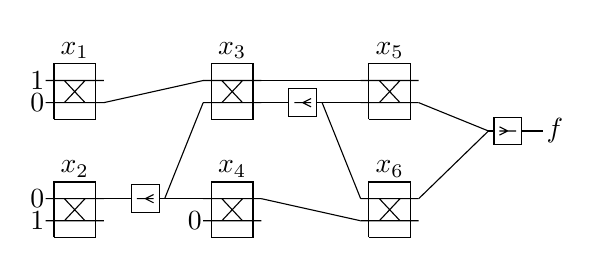
\begin{tikzpicture}
\crossbarat{$x_1$}{0,1.5}{a};
\crossbarat{$x_2$}{0,0}{b};

\crossbarat{$x_3$}{2,1.5}{c};
\crossbarat{$x_4$}{2,0}{d};

\crossbarat{$x_5$}{4,1.5}{e};
\crossbarat{$x_6$}{4,0}{f};

\node[splitter,xshift=15] (splitter) at (b.f) {};
\node[splitter,xshift=15] (splitter2) at (c.g) {};
\node[combiner] (combiner) at (5.5,1) {};
\node[xshift=10,inner sep=1] (fun) at (combiner.out) {$f$};

\draw (b.f) -- (splitter.in);
\draw (splitter.out) -- (d.p);
\draw (e.g) -- (combiner.in);
\draw (a.g) -- (c.p);
\draw (splitter.out) -- (c.q);
\draw (f.f) -- (combiner.in);
\draw (combiner.out) -- (fun);

\draw (c.f) -- (e.p);
\draw (c.g) -- (splitter2.in);
\draw (splitter2.out) -- (e.q);

\draw (splitter2.out) -- (f.p);

\draw (d.f) -- (f.q);

\node[crossin] at (a.p) {$1$};
\node[crossin] at (a.q) {$0$};

\node[crossin] at (b.p) {$0$};
\node[crossin] at (b.q) {$1$};

\node[crossin] at (d.q) {$0$};

\end{tikzpicture}
\caption{Optical circuit}
\label{fig:circuit}
\end{figure}

To measure the complexity of an optical circuit, several metrics got established in the literature~\cite{Condrat2011,WKHD:2015}. More precisely:
\begin{itemize}
\item The number of crossbar gates (often also denoted as gate costs): This metric is  motivated by the fact that each crossbar gate needs to be physically realized. Sometimes, also the number of splitter and the number of combiners are considered. However, as they are significantly easier to realize than the crossbar gates, they are often considered negligible. 

\item The worst case fraction: This metric is motivated by the fact that splitters in the circuit degrade the strength of the involved signal. Since simply counting the number of splitters provides an imprecise measure of the resulting effects (the impact of splitters will significantly differ if, e.g., two splitters separately split two signals or one signal two times in a cascade as shown in Fig.~\ref{fig:split-effect}), a more elaborate metric is considered. First, it is assumed that each splitter with $n$ outputs produces an output signal of strength $\nicefrac{1}{n}$. Then, the circuit's worst case fraction is determined by following all paths from the primary inputs to the primary outputs and multiplying all signal strengths produced by splitters visited on the current path. Afterwards, the maximum value of all paths is considered the worst case fraction\footnote{To keep the model simple, combiners are assumed not to change the signal strength. This makes the worst case fraction a pessimistic approximation i.e. the actual signal strength may be better than the computed one}.
\end{itemize}

\begin{figure}[!h]
\centering
\begin{tikzpicture}
\node[shape=splittergate] (splitter-1) at (0,0) {};
\node[shape=splittergate] (splitter-2) at (0, -1) {};
\node[shape=splittergate] (splitter-3) at (2.5,0) {};
\node[shape=splittergate] (splitter-4) at (3.5,0.5) {};
\node[draw=none] (in1) at (-1,0) {$x_1$};
\node[draw=none] (in2) at (-1,-1) {$x_2$};
\node[draw=none] (in3) at (1.5,0) {$x_3$};
\node[draw=none] (out1) at (1,0.5) {};
\node[draw=none] (out2) at (1,-0.5) {};
\node[draw=none] (out3) at (1,-0.5) {};
\node[draw=none] (out4) at (1,-1.5) {};
\node[draw=none] (out5) at (3,-0.5) {};
\node[draw=none] (out6) at (4.5,1) {};
\node[draw=none] (out7) at (4.5,0) {};

\draw (in1) -- (splitter-1.in);
\draw (in2) -- (splitter-2.in);
\draw (out1) -- (splitter-1.out);
\draw (out2) -- (splitter-1.out);
\draw (out3) -- (splitter-2.out);
\draw (out4) -- (splitter-2.out);
\draw (in3) -- (splitter-3.in);
\draw (splitter-3.out) -- (splitter-4.in);
\draw (out5) -- (splitter-3.out);
\draw (out6) -- (splitter-4.out);
\draw (out7) -- (splitter-4.out);
\end{tikzpicture}
\caption{Impact of splitter}
\label{fig:split-effect}
\end{figure}

\begin{example}
Fig.~\ref{fig:circuit} shows an optical circuit composed of six crossbar gates, two splitters, and
one combiner. The worst case fraction of the circuit is 4.
\end{example}

Although these metrics are just approximations that may not perfectly correspond to the physical
implementation, it gives a better idea of the resulting circuit costs and signal strengths. 

\subsection{Binary Decision Diagram}

Every Boolean function~$f: \B^n \rightarrow \B$ can
be represented by a graph-structure defined as follows:

\begin{definition}
A \emph{Binary Decision Diagram}~(BDD)~\cite{Bryant1986} over Boolean variables~$X$ with terminals $T=\lbrace 0,1\rbrace$ 
is a directed acyclic graph $G=(V,E)$ with the following properties:
\begin{enumerate}
\item Each node $v \in V$ is either a terminal or a non-terminal.
\item Each terminal node $v \in V$ is labeled by a value $t \in T$ and has no outgoing edges.
\item Each non-terminal node $v \in V$ is labeled by a Boolean variable $x_i\in X$ and represents a Boolean function~$f$.
\item In each non-terminal node (labeled by $x_i$), the Shannon decomposition~\cite{Sha:38}
$$f = \overline{x}_if_{x_i=0} + x_if_{x_i=1} $$ %\quad (1 \leq i \leq n)$$
is carried out, leading to two outgoing edges $e \in E$ whose successors 
are denoted by $low(f)$ (for $f_{x_i=0}$) and $high(f)$ (for $f_{x_i=1}$), respectively.
\end{enumerate}
The \emph{size} of a BDD is defined by the number of its (non-terminal) nodes.
\end{definition}

\begin{example}
Fig.~\ref{example:bdd} shows a BDD representing the function $f=x_1 \oplus x_2x_3$. Edges leading to a node $f_{x_i=0}$ ($f_{x_i=1}$) are marked by dashed (solid) lines.
%a~0 (1)
This BDD has a size of~5.
\end{example}

\begin{figure}
\centering
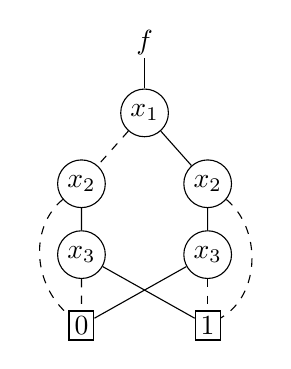
\begin{tikzpicture}[every node/.style={draw,circle,inner sep=2},scale=.6]
\node (ff) {$x_1$}
      child[dashed] {
         node[solid, xshift=-10] (x2) {$x_2$}
         child[solid] {
           node (x3) {$x_3$}
           child[dashed] {
             node[rectangle, solid] (terminal-0) {$0$}
           }
         }
      }
      child[solid] {
       node[solid, xshift=10] (x2-1) {$x_2$}
       child[solid] {
         node (x3-1) {$x_3$}
         child[dashed] {
             node[rectangle, solid] (terminal-1) {$1$}
           }
       }       
      };

\draw (x3) -- (terminal-1);
\draw (x3-1) -- (terminal-0);     
\draw[dashed] (x2) edge[in=140,out=220] (terminal-0);
\draw[dashed] (x2-1) edge[in=30,out=320] (terminal-1);    

\node[above of=ff, draw=none,yshift=-3,inner sep=0] (f) {$f$};  

\draw (ff) -- (f);
\end{tikzpicture}
%\vspace{4cm}
\caption{BDD representing $f=x_1 \oplus x_2x_3$}
\label{example:bdd}  
\end{figure}

A BDD is called \emph{free} if each variable is encountered at
most once on each path from the root to a terminal node. 
A BDD is called \emph{ordered} if in addition all
variables are encountered in the same order on all such paths. 
The respective \emph{order} is defined by
$\pi : \lbrace 1,\dots ,n\rbrace \rightarrow \lbrace 1,\dots ,n\rbrace $.
Finally, a BDD is called \emph{reduced} if it does neither contain isomorphic sub-graphs nor
redundant nodes. To achieve reduced BDDs, \emph{reduction rules} are applied~\cite{Bryant1986}.
Applying the reduction rules leads to \emph{shared nodes}, i.e.~nodes
that have more than one predecessor.

In the following, reduced ordered binary decision diagrams are called BDDs
for brevity. BDDs are canonical representations, i.e.~for a given Boolean function
and a fixed order, the BDD is unique~\cite{Bryant1986}. 


BDDs are very sensitive to the chosen variable order. It has been shown
in~\cite{BW:96} that proving the existence of a BDD with a lower number of nodes 
(i.e.~proving that no other order leads to a smaller BDD size)
%finding the best ordering (i.e.~the ordering leading to the smallest BDD size)
is $\mathcal{NP}$-complete. As a consequence, several heuristics to find good orders have
been proposed. In particular, \emph{sifting}~\cite{Rudell1993} has been shown to be quite effective.

\section{BDD-based Synthesis}\label{sec:bdd-synthesis}

In this section, we briefly review two complementary BDD-based synthesis approaches for optical circuits which have been proposed in the recent past. More precisely, we first discuss the method proposed in~\cite{Condrat2011} followed by its alternative suggested in~\cite{WKHD:2015}. Afterwards, we discuss the drawbacks of these synthesis schemes and their reasons. This eventually provides the motivation for the optimizations proposed in the next section.

\subsection{Gate-Efficient Approach}\label{sec:direct-bdd}

Having a BDD of the function to be realized, a corresponding optical circuit
can easily be derived from it. 
In fact, the Shannon decomposition applied in each BDD node is directly
realized by a crossbar gate as introduced in Def.~\ref{def:crossbar}.
Hence, an optical circuit can be derived by traversing the BDD in a depth-first fashion
and substituting each node~$v\in V$ with a corresponding crossbar gate. 
If a shared node occurs, the respective optical signal has to be split accordingly.
Combining all gates and connecting the respective signals eventually lead to an optical
circuit realizing the desired function.

\begin{example}\label{example:bdd_synth}
Fig.~\subref*{fig:bdd} shows a BDD representing the
function~$f:\mathbbm{B}^5\rightarrow\mathbbm{B}^2$ with \mbox{$f_1=\bar{x}_0x_2+x_0\bar{x}_1x_2+x_0x_1x_4$} and
\mbox{$f_2=\bar{x}_0\bar{x}_1x_2+\bar{x}_0x_1x_4+x_0\bar{x}_3x_4$}.
Fig.~\subref*{fig:bdd_circ} shows the optical circuit obtained from this BDD.
For example, the co-factor represented by the node~$v_d$ can easily be realized by the left-most
crossbar gate shown at the top of Fig.~\subref*{fig:bdd_circ}.
% Note that nodes $v_d$ and $v_f$ are independent of each other, i.e.~either of them can be realized
% first.
Since~this node also represents a shared node, a splitter is added in order to realize the
co-factors represented by~$v_a$ and~$v_c$. In a similar fashion, other nodes are realized which
finally results in the circuit shown in Fig.~\subref*{fig:bdd_circ}.
\end{example}

\begin{figure}
\centering
\subfloat[BDD\label{fig:bdd}]{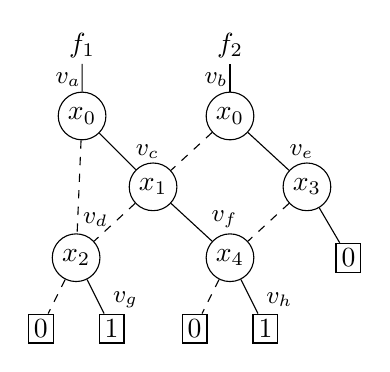
\begin{tikzpicture}[every node/.style={draw,circle,inner
sep=2},scale=.6]
\node (f2) {$x_0$} 
	child[dashed] {
	    node[xshift=-15, solid] (b) {$x_1$}
          child[dashed] {
             node[xshift=-15, solid] (c) {$x_2$} 
              child[dashed] {
                node[rectangle, solid] (zeroTerm) {$0$}
                }
              child[solid] {
                node[rectangle, solid] (term1) {$1$}
                }
              }
              child[solid] {
                  node[xshift=15] (e) {$x_4$}
                   child[dashed] {
                     node[rectangle, solid] {$0$}
                     }
                   child {
                     node[rectangle] (term2) {$1$}
                     }  
                   }
                }
             child {
		node[xshift=15] (d) {$x_3$}
		child { node[rectangle,xshift=15] {$0$} }
	};
\draw[dashed] (d) -- (e);
\node[left of=f2,xshift=-25] (f1) {$x_0$};
\draw (f1) -- (b);
\draw[dashed] (f1) -- (c);

\node[draw=none,yshift=5,xshift=5] at (term1.north) {\small $v_g$};
\node[draw=none,yshift=5,xshift=5] at (term2.north) {\small $v_h$};
\node[draw=none,yshift=5,xshift=7] at (c.north) {\small $v_d$};
\node[draw=none,yshift=5,xshift=-2] at (e.north) {\small $v_f$};
\node[draw=none,yshift=4,xshift=-2] at (d.north) {\small $v_e$};
\node[draw=none,yshift=4,xshift=-2] at (b.north) {\small $v_c$};

\node[above of=f1, draw=none,yshift=-3,inner sep=0] (f1l) {$f_1$};
\node[above of=f2, draw=none,yshift=-3,inner sep=0] (f2l) {$f_2$};

\draw (f1) -- (f1l);
\draw (f2) -- (f2l);

\node[draw=none,yshift=22,xshift=-5] at (f1.south) {\small $v_a$};
\node[draw=none,yshift=22,xshift=-5] at (f2.south) {\small $v_b$};

\end{tikzpicture}}\hspace{.5cm}
\subfloat[Obtained circuit\label{fig:bdd_circ}]{
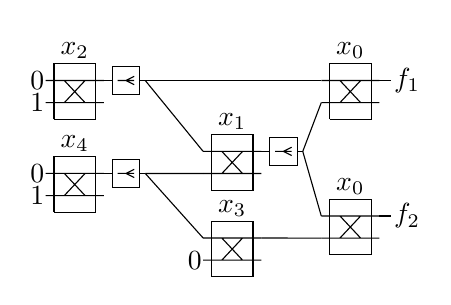
\begin{tikzpicture}
%  \node[crossbar] (x3) at (0,1) {$x_3$};
% 
%  \node[crossbar] (x1) at (1.5,0) {$x_1$};
%  \node[crossbar] (x2) at (1.5,2) {$x_2$};
%  
%  \node[crossbar] (x0_1) at (3,2) {$x_0$};
%  \node[crossbar] (x0_2) at (3,0) {$x_0$};

\crossbarat{$x_2$}{0,2.2}{x2}
\crossbarat{$x_4$}{0,1.02}{x4}
\crossbarat{$x_1$}{2,1.3}{x1}
\crossbarat{$x_3$}{2,0.2}{x3}
\crossbarat{$x_0$}{3.5,2.2}{x0_1}
\crossbarat{$x_0$}{3.5,0.48}{x0_2}

\node[shape=splittergate, xshift=8] (s1) at (x2.f) {};
\node[shape=splittergate, xshift=8] (s2) at (x4.f) {};
\node[shape=splittergate, xshift=8] (s3) at (x1.f) {};

\draw (x2.f) -- (s1.in);
\draw (x4.f) -- (s2.in);
\draw (s1.out) -- (x0_1.p);
\draw (s1.out) -- (x1.p);
\draw (s2.out) -- (x1.q);
\draw (s2.out) -- (x3.p);
\draw (x1.f) -- (s3.in);
\draw (s3.out) -- (x0_1.q);
\draw (s3.out) -- (x0_2.p);
\draw (x3.f) -- (x0_2.q);

\node[crossin] at (x2.p) {$0$};
\node[crossin] at (x2.q) {$1$};
\node[crossin] at (x4.p) {$0$};
\node[crossin] at (x4.q) {$1$};
\node[crossin] at (x3.q) {$0$};

\node[xshift=1em,inner sep=1pt] (f1) at (x0_1.f) {$f_1$};
\node[xshift=1em,inner sep=1pt] (f2) at (x0_2.f) {$f_2$};

\draw (x0_1.f) -- (f1);
\draw (x0_2.f) -- (f2);

%\crossbarat{$x_3$}{0,1}{x3}
%\crossbarat{$x_1$}{1.5,0}{x1}
%\crossbarat{$x_2$}{1.5,2}{x2}
%\crossbarat{$x_0$}{3,2}{x0_1}
%\crossbarat{$x_0$}{3,0}{x0_2}

%\node[shape=splittergate, xshift=8] (s1) at (x3.f) {};
%\node[shape=splittergate, xshift=8] (s2) at (x1.f) {};
%\node[xshift=1em,inner sep=1pt] (f1) at (x0_1.f) {$f_1$};
%\node[xshift=1em,inner sep=1pt] (f2) at (x0_2.f) {$f_2$};

%\draw (x0_1.f) -- (f1);
%\draw (x0_2.f) -- (f2);

%\draw (x3.f) -- (s1.in);
%\draw (s1.out) -- (x2.q);
%\draw (s1.out) -- (x1.p);
%\draw (x2.f) -- (x0_1.p);
%\draw (x1.f) -- (s2.in);
%\draw (s2.out) -- (x0_2.p);
%\draw (s2.out) -- (x0_1.q);

%\node[crossin] at (x3.p) {$0$};
%\node[crossin] at (x3.q) {$1$};
%\node[crossin] at (x2.p) {$1$};
%\node[crossin] at (x0_2.q) {$1$};
%\node[crossin] at (x1.q) {$0$};
\end{tikzpicture}
}
%\caption{BDD(s) representing the boolean function $f$ of Example~\ref{ex:bdd}.}
\caption{Gate-efficient BDD-based synthesis}\label{fig:prev_bdd}
\end{figure}

Considering practically relevant functions, the respective BDD representation
usually includes a large amount of shared nodes which eventually result in splitters. Hence, applying the synthesis
method sketched above leads to optical circuits where certain output signals
are constituted by a negligible fraction of power only. 
%(this is evaluated later in Section~\ref{sec:exp} in detail). 
This is an essential weakness of BDD-based synthesis scheme which makes it unsuitable to be an efficient synthesis approach.

\subsection{Splitter-Free Approach}\label{sec:rev-bdd}

To deal with the problem mentioned above for the direct approach, an alternative has been proposed in~\cite{WKHD:2015}. 
This work shows that BDD-based synthesis still is a suitable scheme -- if applied
in an entirely different fashion.

More precisely, the alternative BDD-based synthesis scheme exploits
the fact that a function~$f$ to be realized is defined by the~1-paths of the
corresponding BDD. A \emph{1-path}
$p=(v_1,v_2,\dots , v_l)$ with $v_i\in V$  
for a given BDD~$G=(V,E)$ representing~$f$ is a sequence of nodes obtained by traversing the
BDD from the root node to a \tikz{\node[rectangle,draw,scale=0.7] {1};}-terminal. 
A single path can be realized, as described in Section~\ref{sec:direct-bdd},
i.e.~by simply traversing each node of the path and adding a corresponding crossbar gate.
Based on that, a given function~$f$ can be realized by separately
synthesizing all \mbox{1-paths} of the corresponding BDD and eventually ORing the respective 
outputs\footnote{Note that ORing optical signals can be realized
by a single combiner, i.e.~the output of the combiner emits light~(i.e.~the logical value~1)
if at least one of its optical inputs sources light.}

However, generating optical logic for all \mbox{1-paths} separately 
obviously would lead to a very expensive circuit
realization. Hence, another property is exploited: 
the direction in which a \mbox{1-path} is traversed during synthesis does not matter, 
i.e.~the path can be traversed from the root node to the 
\mbox{\tikz{\node[rectangle,draw,scale=0.7] {1};}-terminals} or vice versa. 
In contrast to straight-forward BDD schemes, 
it has been proposed to traverse the \mbox{1-paths} in a
\emph{reverse} fashion, i.e.~from the root nodes to the \mbox{\tikz{\node[rectangle,draw,scale=0.7]
{1};}-terminals}. By this, shared nodes of the BDD can fully be exploited, i.e.~no redundant logic
has to be created, while, at the same time, combiners instead of splitters can be applied for
their realization. This reduces the number of cases an optical signal is split to zero and, hence,
overcomes the weakness of BDD-based synthesis reviewed in Section~\ref{sec:direct-bdd}.

The following example illustrates the idea.

\begin{example}\label{ex:reverse}
Consider again the function~$f_1$ as discussed in Example~\ref{example:bdd_synth}.
Its corresponding BDD is shown at the left-hand side of Fig.~\subref*{fig:bdd_reverse}.
The bold edges indicate the three $1$-paths.
Considering these paths in the direction from the root to the terminals yields the two
functions~$f'_1=x_2 (\overline{x_0}\vee x_0\overline{x_1})$ and~$f''_1=x_0x_1x_4$ with
$f'_1\vee f''_1=f_1$.
This interpretation of the BDD can be realized without any splitters as
shown at the top of Fig.~\subref*{fig:bdd_circ_reverse}. Following the $1$~signal through the
circuit corresponds directly to the $1$-paths of the BDD.
\end{example}

\tikzset{ulabel/.style={draw=none,xshift=5,yshift=-4}}
\begin{figure}[!h]
\centering
\subfloat[BDD(s) for $f_1=f_1'\vee f_1''$ and $f_2=f_2' \vee f_2''$\label{fig:bdd_reverse}]{
\begin{tikzpicture}[every node/.style={draw,circle,inner sep=2},scale=.6,]
\node[xshift=-70] (f1) {$x_0$}
    child[dashed] {
           node[yshift=-25, solid] (x2) {$x_2$}
             child { node[rectangle, solid] {$0$} }
             child { node[inner sep=1,draw=none] (f11) {
			\begin{tikzpicture}[scale=0.8]
				\node[rectangle] {$1$};
			\end{tikzpicture} }
         } 
       } 
      child {
       node (x1) {$x_1$}
         child {
           node[xshift=15] (x4) {$x_4$}
             child[dashed] { node[rectangle, solid] {$0$} }
             child { node[inner sep=1,draw=none] (f12) {
			         \begin{tikzpicture}[scale=0.8]
				         \node[rectangle, dashed] {$1$};
			          \end{tikzpicture} }
         }
        }    
    };
\draw[very thick] (x2) -- (f11);
\draw[dashed, very thick] (x1) -- (x2);
\draw[very thick] (x4) -- (f12);
\draw[very thick] (x1) -- (x4);
\draw[very thick] (f1) -- (x1);
\draw[dashed, very thick] (f1) -- (x2);

\node[above of=f1, draw=none,yshift=-3,inner sep=0] (f1l) {$f_1$};

\draw[very thick] (f1) -- (f1l);
\draw (f1l.south west) -- (f1l.north east);

\node[ulabel,xshift=-10,yshift=-3] (term11) at (f11.south east) {$\pmb{f_1'}$};
\node[ulabel,xshift=-10,yshift=-3] (term12) at (f12.south east) {$\pmb{f_1''}$};

\node[rectangle,xshift=5] (term3) at (f1l.south east) {$\pmb{1}$};

\draw (f11.south west) -- (f11.north east);
\draw (f12.south west) -- (f12.north east);

\node[right of=f1,xshift=70] (f2) {$x_0$}
	child[dashed] {
		node[solid] (x11) {$x_1$}
		child[dashed] {
			node[solid] (x12) {$x_2$}
			child { node[rectangle, solid] {$0$} }
			child { node[inner sep=1,draw=none] (f21) {
				\begin{tikzpicture}[scale=0.8]
					\node[rectangle] {$1$};
				\end{tikzpicture}
				}
			}
		}
		child {
		  node[xshift=15, solid] (x14) {$x_4$}
		   child { node[rectangle, solid] {$0$} }
		   child { node[inner sep=1,draw=none] (f22) {
				\begin{tikzpicture}[scale=0.8]
					\node[rectangle] {$1$};
				\end{tikzpicture}
				}
		      }
		 }  
	}	     		
	child { node[xshift=15] (x13) {$x_3$}
	     child { node[rectangle, xshift=20] {$0$} }
	};

\draw[very thick] (x14) -- (f22);
\draw[very thick] (x12) -- (f21);
\draw[dashed, very thick] (x11) -- (x12);
\draw[very thick] (x11) -- (x14);
\draw[dashed, very thick] (x13) -- (x14);
\draw[very thick] (x13) -- (f2);
\draw[dashed, very thick] (f2) -- (x11);

\node[above of=f2, draw=none,yshift=-3,inner sep=0] (f2l) {$f_2$};

\draw[very thick] (f2) -- (f2l);
\draw (f2l.south west) -- (f2l.north east);

\node[ulabel,xshift=-10,yshift=-3] (term21) at (f21.south east) {$\pmb{f_2'}$};
\node[ulabel,xshift=-10,yshift=-3] (term22) at (f22.south east) {$\pmb{f_2''}$};

\node[rectangle,xshift=5] (term4) at (f2l.south east) {$\pmb{1}$};

\draw (f21.south west) -- (f21.north east);
\draw (f22.south west) -- (f22.north east);

\end{tikzpicture}}
\vspace{0.2cm}
\subfloat[Obtained circuit(s)\label{fig:bdd_circ_reverse}]{
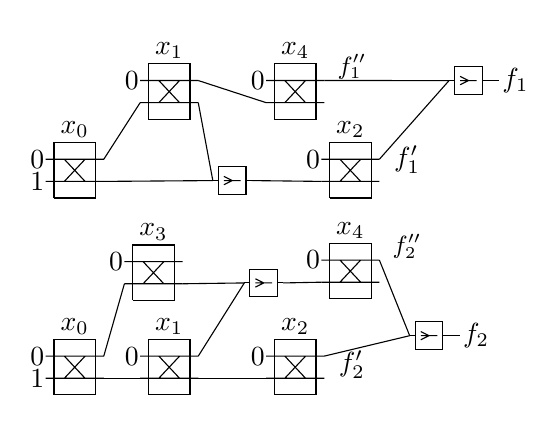
\begin{tikzpicture}
\begin{scope}[yshift=2.5cm]
\crossbarat{$x_0$}{0,1}{x0}
\crossbarat{$x_1$}{1.2,2}{x1}
\crossbarat{$x_4$}{2.8,2}{x4}
\crossbarat{$x_2$}{3.5,1}{x2}

\node[combiner] (com1) at (2,0.87) {};
\node[combiner] (com2) at (5,2.14) {};

\draw (x0.f) -- (x1.q);
\draw (x0.g) -- (com1.in);
\draw (x1.g) -- (com1.in);
\draw (com1.out) -- (x2.q);
\draw (x1.f) -- (x4.q);
\draw (x2.f) -- (com2.in);
\draw (x4.f) -- (com2.in);

\node[crossin] at (x0.p) {$0$};
\node[crossin] at (x0.q) {$1$};
\node[crossin] at (x1.p) {$0$};
\node[crossin] at (x4.p) {$0$};
\node[crossin] at (x2.p) {$0$};

\node[xshift=1em,yshift=0.5em,inner sep=1pt] (f11) at (x4.f) {\small $f_1''$};
\node[xshift=1em,inner sep=1pt] (f12) at (x2.f) {$f_1'$};

\node[xshift=10,inner sep=1] (f1) at (com2.out) {$f_1$};

\draw (com2.out) -- (f1);
\end{scope}

%% circuit for f2

\crossbarat{$x_0$}{0,1}{x0}
\crossbarat{$x_1$}{1.2,1}{x1}
\crossbarat{$x_2$}{2.8,1}{x2}
\crossbarat{$x_3$}{1,2.2}{x3}
\crossbarat{$x_4$}{3.5,2.22}{x4}

\node[combiner] (com1) at (2.4,2.07) {};
\node[combiner] (com2) at (4.5,1.4) {};

\draw (x0.f) -- (x3.q);
\draw (x0.g) -- (x1.q);
\draw (x1.g) -- (x2.q);
\draw (x3.g) -- (com1.in);
\draw (x1.f) -- (com1.in);
\draw (com1.out) -- (x4.q);
\draw (x2.f) -- (com2.in);
\draw (x4.f) -- (com2.in);

\node[crossin] at (x0.p) {$0$};
\node[crossin] at (x0.q) {$1$};
\node[crossin] at (x1.p) {$0$};
\node[crossin] at (x3.p) {$0$};
\node[crossin] at (x4.p) {$0$};
\node[crossin] at (x2.p) {$0$};

\node[xshift=1em,yshift=0.5em,inner sep=1pt] (f21) at (x4.f) {\small $f_2''$};
\node[xshift=1em,yshift=-0.3em,inner sep=1pt] (f22) at (x2.f) {$f_2'$};

\node[xshift=10,inner sep=1] (f2) at (com2.out) {$f_2$};

\draw (com2.out) -- (f2);

\end{tikzpicture}}

%\caption{BDD(s) representing the boolean function $f$ of Example~\ref{ex:bdd}.}
\caption{Reverse BDD-based synthesis}\label{fig:reverse_bdd}
\end{figure}

This reverse BDD-based synthesis can only be applied to BDDs
representing functions \mbox{$f:\B^n\rightarrow \B^1$,} i.e.~functions with one
output only.
In order to realize multi-output functions such as considered in Example~\ref{example:bdd_synth},
all respective outputs have to be treated separately. The right-hand side of Fig.~\ref{fig:bdd_reverse}
and the bottom of Fig.~\ref{fig:bdd_circ_reverse} show the 
BDD and the resulting circuit for the function~$f_2$
considered in Example~\ref{example:bdd_synth}, respectively. This restriction, of course, prevents 
the full exploitation of sharing among functions within the BDD.
Since additional BDD nodes directly translate to additional crossbar gates, this eventually leads to an overhead of crossbar gates.

\section{BDD Optimization}

\subsection{Motivation}

\newpage

\subsection{Exploiting BDD Optimization}


%\section{Discussion and Motivation\sectionmark{Motivation}}~\label{sec:motivation-for-bdd-opt}

As discussed, both approaches have their own limitations: While direct BDD-based synthesis generates circuits with many splitters (and, hence, huge worst case fractions), the reverse BDD-based synthesis produces circuits with redundant gates. In order to minimize the number of splitters and redundant gates in optical circuits, the BDD structure needs to be optimized with respect to shared nodes and one-paths.   
%The BDD-based synthesis methods reviewed above show that the complexity of the decision diagram has a significant influence on the resulting optical circuits. 
More precisely,

\begin{itemize}

\item In direct BDD-based synthesis, sharing of a node is realized using a splitter. Moreover, the output signal power decreases whenever, a signal is split. Therefore, it appears that the number of shared nodes in a BDD significantly influences two complexity metrics of optical circuits: the number of splitters and the worst case fraction. In order to reduce the number of splitters and improve the worst case fraction, the amount of shared nodes in the corresponding BDD structure needs to be minimized.

\item In BDDs,  common sub-functions are shared among multiple output functions by a single path. In case of reverse BDD-based synthesis, since each function is considered individually, therefore, the common one-path among multiple functions can not be treated at once. As a result, these one-paths are realized for every functions which ultimately lead to redundant crossbar gates in the resulting optical circuits. Therefore, if the number of one-paths is reduced, then, the number of gates can be reduced which in turn will minimize the additional gate overhead. 
\end{itemize}

In the following sections, we propose the utilization of BDD minimization in order to address these objectives and, afterwards, discuss their effect on the optical circuits in detail.   

%\section{Exploiting BDD Optimization\sectionmark{BDD Optimization}}\label{sec:bdd-minimization}

In general, BDD optimization involves the determination of a ``good'' variable ordering which minimizes the complexity of the BDD. In the present context, the complexity refers to the number of shared nodes and the number of one-paths in the BDD. This section presents how corresponding optimization techniques can be used for optimizing optical circuits. 

\subsubsection{Determining a Good Variable Order}

Searching for a good variable order requires the consideration of different permutations of variables until a BDD with a small (ideally the smallest) complexity results. Sifting~\cite{Rudell1993} is one such technique which orders the variables in a fashion to minimize the number of nodes in a BDD. The general idea behind this approach is to select and move a variable to any position based on swapping of adjacent variables. Then, the currently considered variable is fixed at the best position (i.e.~where a minimum number of nodes resulted) and the next variable is considered. This way, no variable is selected more than once which guarantees an efficient procedure while providing rather good results.

In our context, the technique of sifting can be modified so that it serves the purpose of optical circuit optimization. 
In fact, we are not primarily interested in reducing the number of nodes in the BDD but, as discussed above, the number of shared nodes or the number of one-paths.
This can be accomplished by modifying the objective function of the sifting algorithm accordingly.

The basic working principle of sifting is adapted by many other algorithms~\cite{Bollig95,FeyD06,ShirinzadehSD15} which provide better solutions compared to sifting, however, not in reasonable run-time. 
In this work, we are not aiming to use minimal BDDs with respect to the optimization objectives. But we shall exploit the benefits of 
optimization whose priority is given towards the minimal solution. Taking this into consideration, a BDD minimization reported recently in~\cite{ShirinzadehSD15} is used for 
determining a suitable variable order. 
More precisely, we took the schemes presented there, but adjusted them so that either the number of shared nodes or the number of one-paths are reduced.
Afterwards, we evaluated whether this leads to more efficient optical circuits. 
The following two sub-sections illustrate these issues in more detail.

%\subsection{Direct BDD-based Synthesis with Shared Node Minimization}
\subsection{Reducing Splitters in Gate-Efficient Circuits}


To obtain an optical circuit from a given BDD, first the number of shared nodes in the corresponding BDD is minimized. This is achieved by setting the objective function of~\cite{ShirinzadehSD15} as shared node.  %using an evolutionary algorithm. 
Once the minimum number of shared nodes is obtained, an optical circuit is derived out of the optimized BDD using direct BDD-based approach.

\begin{example}
Consider the following function: $$g=\bar{x}_0\bar{x}_1\bar{x}_2x_3+x_0x_1\bar{x}_2x_4+x_1\bar{x}_3\bar{x}_4+x_0
\bar{x}_2x_3+x_2\bar{x}_3x_4+x_0\bar{x}_1\bar{x}_3x_4.$$ 
The corresponding BDD\footnote{For sake of clarity, the paths leading to zero terminal are omitted from rest of the BDD figures.} structure contains 3 shared nodes as depicted in Fig.~\ref{fig:bdd-g}. As a result, the generated optical circuit shown in Fig.~\ref{fig:bdd-circ-g} contains 3 splitters. Applying  shared node optimization using the evolutionary algorithm, the number of shared nodes in the BDD can be reduced from 3 to 1 (as appears in Fig.~\ref{fig:min-bdd-g}). This allows for the synthesis of a significantly improved optical  circuit as depicted in Fig.~\ref{fig:min-bdd-circ-g}. Here, the number of splitters in the optical circuit is reduced by the same amount as that of the shared nodes. Moreover, this reduction also causes a decrease in the worst case fraction from 4 to 2 and, eventually, leads to a much better signal strength at the output of the circuit.
\end{example}

\begin{figure}[!h]
\subfloat[Original BDD\label{fig:bdd-g}]{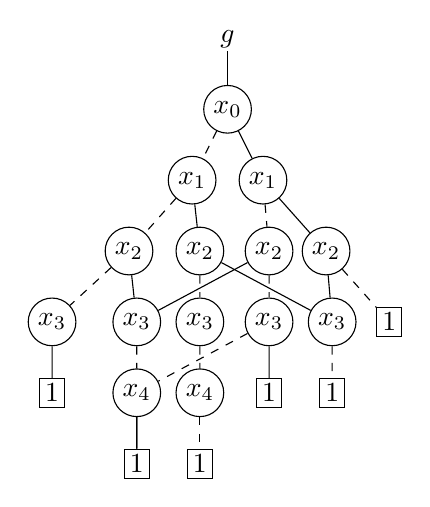
\begin{tikzpicture}[every node/.style={draw,circle,inner
sep=2},scale=.6]
\node (f1) {$x_0$} 
	child[dashed] {
		node[solid] (x1-1) {$x_1$}
		child[dashed] {
			node[solid,xshift=-10] (x2-1) {$x_2$}
			child[dashed] {
			    node[solid, xshift = -15] (x3-2){$x_3$}
			     %child[dashed] {
			      %  node[rectangle,solid] (zeroterm) {$0$}
			     %}
			     child[solid] {
			        node[rectangle] (term1-1) {$1$}
			     }
			}
			child[solid] {
			    node[xshift=-10] (x3-3) {$x_3$}
			    child[dashed] {
			      node[solid] (x4-2) {$x_4$}
			      child[solid] {
			        node[rectangle] (oneterm) {$1$}
			      }    
		        }
		    } 
		 }      
		 child[solid] {
			node[xshift=-10] (x2-2) {$x_2$}
			  child[dashed] {
				node[solid] (x3-1) {$x_3$}
				 child {
				   node[solid] (x4-1) {$x_4$}
				    child {
				      node[rectangle,solid] (term1-5) {$1$}
	   			 }
	   			 }
			  }
		}
	}
	child {
		   node (x1-2) {$x_1$}
		   child[dashed] {
		      node[solid,xshift=15] (x2-3) {$x_2$}
		      child[dashed] {
		        node[solid] (x3-4) {$x_3$}
		         child[solid] {
		           node[rectangle] (term1-4) {$1$}
		        }
		      }
			}
			child {
			  node[xshift=10] (x2-4) {$x_2$}
			  child {
			    node[xshift=15] (x3-5) {$x_3$}
			    child[dashed] {
			      node[solid,rectangle] (term1-2) {$1$}
			    }
			}
			child[dashed] {
			      node[solid,rectangle,xshift=10] (term1-3) {$1$}
			}
		}
	};
		
%\draw[dashed] (x4-1) -- (oneterm);
%\draw (x4-1) -- (zeroterm);
%\draw (x3-1) -- (zeroterm);
%\draw (x3-2) -- (oneterm);
%\draw (x3-5) -- (zeroterm);
%\draw[dashed] (x3-5) -- (oneterm);
\draw (x4-2) -- (oneterm);
%\draw[dashed] (x4-2) -- (zeroterm);
%\draw (x3-4) -- (oneterm);
\draw[dashed] (x3-4) -- (x4-2);
\draw (x2-3) -- (x3-3); 
%\draw[dashed] (x2-4) -- (oneterm);
\draw (x2-2) -- (x3-5);

\node[above of=f1, draw=none,yshift=-3,inner sep=0] (f1l) {$g$};

\draw (f1) -- (f1l);
\end{tikzpicture}}\hspace{0.7cm}
\subfloat[Resulting circuit\label{fig:bdd-circ-g}]{
\resizebox{.6\textwidth}{!}{
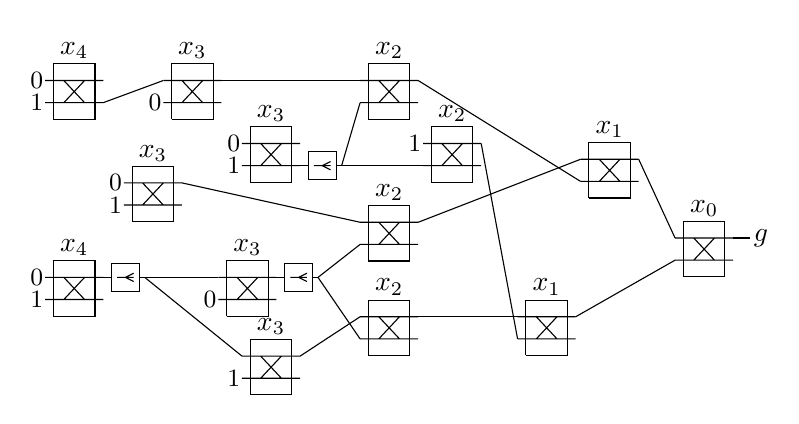
\begin{tikzpicture}
\crossbarat{$x_4$}{0,1}{x4-1}
\crossbarat{$x_3$}{1.5,1}{x3-1}
\crossbarat{$x_3$}{1,-0.3}{x3-2}
\crossbarat{$x_4$}{0,-1.5}{x4-2}
\crossbarat{$x_3$}{2.2,-1.5}{x3-3}
\crossbarat{$x_3$}{2.5,-2.5}{x3-4}
\crossbarat{$x_2$}{4,-0.8}{x2-2}
\crossbarat{$x_2$}{4,-2}{x2-3}
\crossbarat{$x_3$}{2.5,0.2}{x3-5}
\crossbarat{$x_2$}{4,1}{x2-1}
\crossbarat{$x_2$}{4.8,0.2}{x2-4}
\crossbarat{$x_1$}{6.8,0}{x1-1}
\crossbarat{$x_1$}{6,-2}{x1-2}
\crossbarat{$x_0$}{8,-1}{x0}

\node[shape=splittergate, xshift=8] (s1) at (x4-2.f) {};
\node[shape=splittergate, xshift=8] (s2) at (x3-3.f) {};
\node[shape=splittergate, xshift=8] (s3) at (x3-5.g) {};

\draw (x4-1.g) -- (x3-1.p);
\draw (x4-2.f) -- (s1.in);
\draw (s1.out) -- (x3-3.p);
\draw (s1.out) -- (x3-4.p);
\draw (x3-3.f) -- (s2.in);
\draw (x3-2.f) -- (x2-2.p);
\draw (s2.out) -- (x2-2.q);
\draw (s2.out) -- (x2-3.q);
\draw (x3-4.f) -- (x2-3.p);
\draw (x3-5.g) -- (s3.in);
\draw (x3-1.f) -- (x2-1.p);
\draw (s3.out) -- (x2-1.q);
\draw (s3.out) -- (x2-4.q);
\draw (x2-4.f) -- (x1-2.q);
\draw (x2-3.f) -- (x1-2.p);
\draw (x2-1.f) -- (x1-1.q);
\draw (x2-2.f) -- (x1-1.p);
\draw (x1-1.f) -- (x0.p);
\draw (x1-2.f) -- (x0.q);


\node[crossin] at (x4-1.p) {\small $0$};
\node[crossin] at (x4-1.q) {\small $1$};
\node[crossin] at (x3-1.q) {\small $0$};
\node[crossin] at (x3-2.p) {\small $0$};
\node[crossin] at (x3-2.q) {\small $1$};
\node[crossin] at (x4-2.p) {\small $0$};
\node[crossin] at (x4-2.q) {\small $1$};
\node[crossin] at (x3-3.q) {\small $0$};
\node[crossin] at (x3-4.q) {\small $1$};
\node[crossin] at (x3-5.p) {\small $0$};
\node[crossin] at (x3-5.q) {\small $1$};
\node[crossin] at (x2-4.p) {\small $1$};

\node[xshift=1em,inner sep=1pt] (f) at (x0.f) {$g$};

\draw (x0.f) -- (f);
\end{tikzpicture}}}\hspace{1cm}
\subfloat[BDD with minimized shared nodes\label{fig:min-bdd-g}]{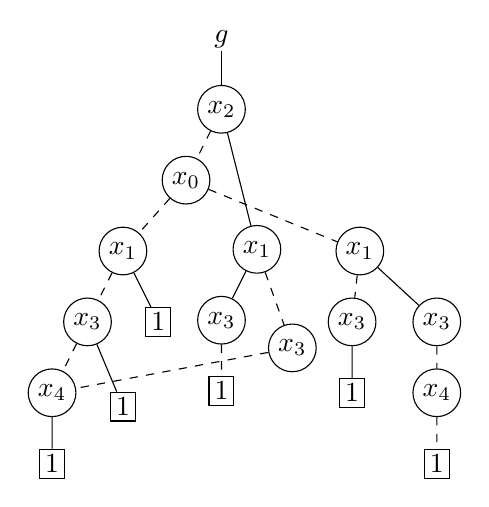
\begin{tikzpicture}[every node/.style={draw,circle,inner
sep=2},scale=.6]
\node (f1) {$x_2$} 
	child[dashed] {
		node[solid] (x0) {$x_0$}
		 child {
			node[solid,xshift=-10] (x1-1) {$x_1$}
			child[dashed] {
			    node[solid] (x3-1){$x_3$}
			    child[dashed] {
			       node[solid] (x4-1) {$x_4$}
			       child[solid] {
			         node[rectangle] (oneterm) {$1$}
			       }
			    }
			    child[solid] {
			         node[rectangle,yshift=-5] (term1-2) {$1$}
			       }
			}
			child[solid] { 
			  node[rectangle] (term1-1) {$1$}
			 }
		}	
		child[dashed] {
			node[solid,xshift=50] (x1-3) {$x_1$}
			child[dashed] {
			  node[solid,xshift=10] (x3-4) {$x_3$}
			  child[solid] { 
			  node[rectangle] (term1-4) {$1$}
			 }
			}
			child[solid] {
			  node[solid,xshift=15] (x3-5) {$x_3$}
			  child[dashed] {
			    node[solid] (x4-2) {$x_4$}
			    child {
			       node[rectangle,solid] (term1-3) {$1$}
			    }
			  }
			}
		}    
	}
	child {
	  node[yshift=-25] (x1-2) {$x_1$}
	  child {
	    node (x3-2) {$x_3$}
	    child[dashed] { 
			  node[rectangle,solid] (term1-6) {$1$}
			 }
	  }
	  child[dashed] {
	    node[solid,yshift=-10] (x3-3) {$x_3$}
	  }
	};
				
%\draw (x3-1) -- (oneterm);
%\draw (x1-1) -- (oneterm);
%\draw[dashed] (x3-4) -- (zeroterm);
%\draw (x3-4) -- (oneterm);
%\draw[dashed] (x4-2) -- (oneterm);
%\draw[dashed] (x4-1) -- (zeroterm);
%\draw (x3-5) -- (zeroterm);
%\draw[dashed] (x3-2) -- (oneterm);
%\draw (x3-2) -- (zeroterm);
%\draw (x3-3) -- (zeroterm);
\draw[dashed] (x3-3) -- (x4-1);


\node[above of=f1, draw=none,yshift=-3,inner sep=0] (f1l) {$g$};

\draw (f1) -- (f1l);

\end{tikzpicture}}\hspace{.5cm}
\subfloat[Resulting circuit\label{fig:min-bdd-circ-g}]{
\resizebox{.5\textwidth}{!}{
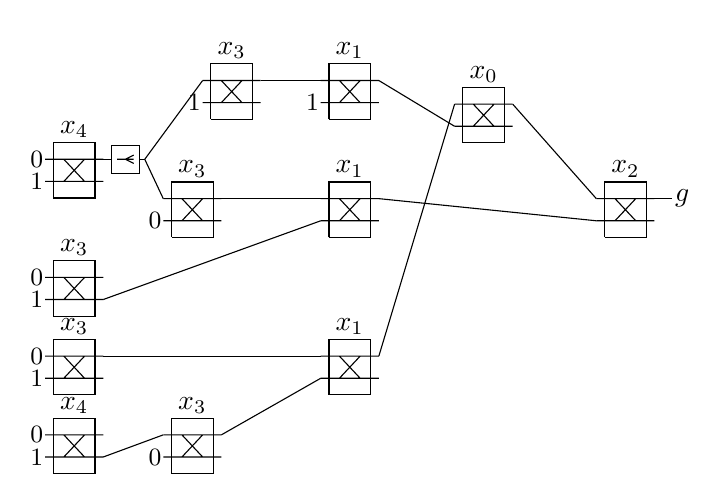
\begin{tikzpicture}
\crossbarat{$x_4$}{0,1}{x4-1}
\crossbarat{$x_3$}{2,2}{x3-1}
\crossbarat{$x_3$}{1.5,0.5}{x3-2}
\crossbarat{$x_3$}{0,-0.5}{x3-3}
\crossbarat{$x_3$}{0,-1.5}{x3-4}
\crossbarat{$x_3$}{1.5,-2.5}{x3-5}
\crossbarat{$x_4$}{0,-2.5}{x4-2}
\crossbarat{$x_1$}{3.5,2}{x1-1}
\crossbarat{$x_1$}{3.5,0.5}{x1-2}
\crossbarat{$x_1$}{3.5,-1.5}{x1-3}
\crossbarat{$x_0$}{5.2,1.7}{x0}
\crossbarat{$x_2$}{7,0.5}{x2}

\node[shape=splittergate, xshift=8] (s1) at (x4-1.f) {};

\draw (x4-1.f) -- (s1.in);
\draw (s1.out) -- (x3-2.p);
\draw (s1.out) -- (x3-1.p);
\draw (x3-3.g) -- (x1-2.q);
\draw (x3-2.f) -- (x1-2.p);
\draw (x3-1.f) -- (x1-1.p);
\draw (x4-2.g) -- (x3-5.p);
\draw (x3-4.f) -- (x1-3.p);
\draw (x3-5.f) -- (x1-3.q);
\draw (x1-3.f) -- (x0.p);
\draw (x1-1.f) -- (x0.q);
\draw (x0.f) -- (x2.p);
\draw (x1-2.f) -- (x2.q);

\node[crossin] at (x4-1.p) {\small $0$};
\node[crossin] at (x4-1.q) {\small $1$};
\node[crossin] at (x3-1.q) {\small $1$};
\node[crossin] at (x3-2.q) {\small $0$};
\node[crossin] at (x3-3.p) {\small $0$};
\node[crossin] at (x3-3.q) {\small $1$};
\node[crossin] at (x3-4.p) {\small $0$};
\node[crossin] at (x3-4.q) {\small $1$};
\node[crossin] at (x1-1.q) {\small $1$};
\node[crossin] at (x4-2.p) {\small $0$};
\node[crossin] at (x4-2.q) {\small $1$};
\node[crossin] at (x3-5.q) {\small $0$};

\node[xshift=1em,inner sep=1pt] (f) at (x2.f) {$g$};

\draw (x2.f) -- (f);
\end{tikzpicture}}}
\caption{Direct BDD-based synthesis with shared node optimization}\label{fig:direct-bdd-g}
\end{figure}

While shared node reduction definitely reduces the number of splitters in the optical circuits, it does not always guarantee fraction minimization. This is because the fraction depends on the number of fan-out of the splitter, which in turn, depends on the number of times a node is shared. That is, if the number of shared nodes decreases, on the other hand, the sharing of a node increases, this may lead to optical circuits with reduced splitters but increased fraction. This is illustrated with following example.
   
\begin{example}\label{ex:increase_in_fraction}
Consider the function:
%\parbox{\textwidth}{}
$$h=\bar{x}_0\bar{x}_1\bar{x}_2x_3+\bar{x}_0\bar{x}_1x_2\bar{x}_3+\bar{x}_0x_1
\bar{x}_2\bar{x}_3+\bar{x}_0x_1x_2x_3+x_0\bar{x}_1\bar{x}_2\bar{x}_3+x_0\bar{x}_1x_2x_3+
x_0x_1\bar{x}_2x_3 +x_0x_1x_2\bar{x}_3.$$
The BDD of the function is shown in Fig.\ref{fig:bdd-h}. Accordingly, there are 3 shared nodes with each being shared twice. The corresponding optical circuit as shown in Fig.~\ref{fig:bdd-circ-h} has 3 splitters with a worst case fraction of 4. After applying shared node minimization, the resulting BDD contains 2 shared nodes as shown in Fig.~\ref{fig:min-bdd-h}. However, one node is shared 3 times. As a result, the generated optical circuit (depicted in Fig.~\ref{fig:min-bdd-circ-h}) contains 2 splitters but has a worst case fraction of~6. Therefore, the optimization reduces the splitter from 3 to 2, but increases the fraction value from 4 to 6.
\end{example}

\begin{figure}[!h]
\centering
\subfloat[Original BDD\label{fig:bdd-h}]{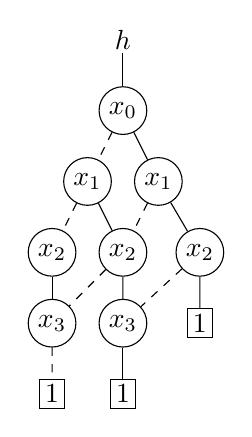
\begin{tikzpicture}[every node/.style={draw,circle,inner
sep=2},scale=.6]
\node (f1) {$x_0$} 
	child[dashed] {
		node[solid] (cx1) {$x_1$}
		child[dashed] {
			node[solid] (cx2) {$x_2$}
			child[solid] {
			    node (rx3-1){$x_3$}
			    child[dashed] {
				   node[rectangle,solid] (term1) {$1$}
				}
			}
			%child[dashed] {
			 %   node[rectangle, solid] (zeroterm) {$0$}
			%}    
		}
		child[solid] {
			node (rx2-1) {$x_2$}
			child[solid] {
				node (rx3-2) {$x_3$}
				child {
				   node[rectangle] (oneterm) {$1$}
				}
			}
		}
		}
		child {
		   node (rx1) {$x_1$}
		   child {
		      node[xshift=15] (rx2-2) {$x_2$}
		      child {
				   node[rectangle] (term3) {$1$}
				}
			}
		};
		
\draw[dashed] (rx1) -- (rx2-1);
\draw[dashed] (rx2-1) -- (rx3-1);
%\draw (rx3-1) -- (zeroterm);
%\draw[dashed] (rx3-1) -- (oneterm);
\draw[dashed] (rx2-2) -- (rx3-2);
%\draw (rx2-2) -- (oneterm);
%\draw[dashed] (rx3-2) -- (zeroterm);

\node[above of=f1, draw=none,yshift=-3,inner sep=0] (f1l) {$h$};

\draw (f1) -- (f1l);
\end{tikzpicture}}\hspace{.5cm}
\subfloat[Resulting circuit\label{fig:bdd-circ-h}]{
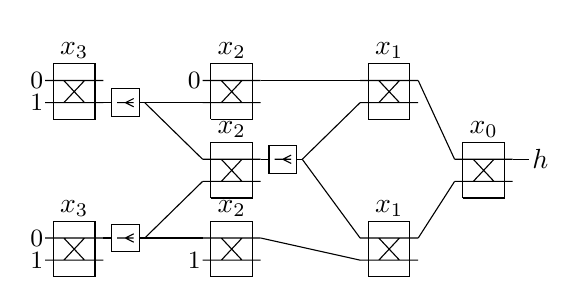
\begin{tikzpicture}
\crossbarat{$x_3$}{0,1}{x3-1}
\crossbarat{$x_3$}{0,-1}{x3-2}
\crossbarat{$x_2$}{2,1}{x2-1}
\crossbarat{$x_2$}{2,0}{x2-2}
\crossbarat{$x_2$}{2,-1}{x2-3}
\crossbarat{$x_1$}{4,1}{x1-1}
\crossbarat{$x_1$}{4,-1}{x1-2}
\crossbarat{$x_0$}{5.2,0}{x0}

\node[shape=splittergate, xshift=8] (s1) at (x3-1.g) {};
\node[shape=splittergate, xshift=8] (s2) at (x3-2.f) {};
\node[shape=splittergate, xshift=8] (s3) at (x2-2.f) {};

\draw (x3-1.g) -- (s1.in);
\draw (x3-2.f) -- (s2.in);
\draw (s1.out) -- (x2-1.q);
\draw (s1.out) -- (x2-2.p);
\draw (s2.out) -- (x2-2.q);
\draw (s2.out) -- (x2-3.p);
\draw (x2-2.f) -- (s3.in);
\draw (x2-1.f) -- (x1-1.p);
\draw (s3.out) -- (x1-1.q);
\draw (s3.out) -- (x1-2.p);
\draw (x2-3.f) -- (x1-2.q);
\draw (x1-1.f) -- (x0.p);
\draw (x1-2.f) -- (x0.q);


\node[crossin] at (x3-1.p) {\small $0$};
\node[crossin] at (x3-1.q) {\small $1$};
\node[crossin] at (x3-2.p) {\small $0$};
\node[crossin] at (x3-2.q) {\small $1$};
\node[crossin] at (x2-1.p) {\small $0$};
\node[crossin] at (x2-3.q) {\small $1$};

\node[xshift=1em,inner sep=1pt] (f) at (x0.f) {$h$};

\draw (x0.f) -- (f);
\end{tikzpicture}}\hspace{0.5cm}
\subfloat[BDD with minimized shared nodes\label{fig:min-bdd-h}]{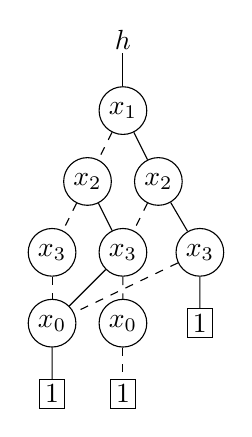
\begin{tikzpicture}[every node/.style={draw,circle,inner
sep=2},scale=.6]
\node (f1) {$x_1$} 
	child[dashed] {
		node[solid] (cx2) {$x_2$}
		child[dashed] {
			node[solid] (cx3-1) {$x_3$}
			child[dashed] {
			    node[solid] (cx0-1){$x_0$}
			    child[solid] {
			        node[rectangle] (term1) {$1$}
			    }    
			}
			%child {
			 %   node[rectangle] (zeroterm) {$0$}
			%}    
		}
		child[solid] {
			node (rx3-1) {$x_3$}
			child[dashed] {
				node[solid] (cx0-2) {$x_0$}
				child[dashed] {
				   node[rectangle, solid] (term2) {$1$}
				}
			}
		}
	}
	child {
	    node (rx2) {$x_2$}
		child {
		   node[xshift=15] (rx3-2) {$x_3$}
		   child[solid] {
				node[rectangle] (term3) {$1$}
		   }
		}
	};
		
\draw[dashed] (rx2) -- (rx3-1);
\draw (rx3-1) -- (cx0-1);
%\draw[dashed] (cx0-1) -- (zeroterm);
%\draw (cx0-1) -- (oneterm);
\draw[dashed] (rx3-2) -- (cx0-1);
%\draw (cx0-2) -- (zeroterm);
%\draw[dashed] (cx0-2) -- (oneterm);
%\draw (rx3-2) -- (oneterm);

\node[above of=f1, draw=none,yshift=-3,inner sep=0] (f1l) {$h$};

\draw (f1) -- (f1l);

\end{tikzpicture}}\hspace{.5cm}
\subfloat[Resulting circuit\label{fig:min-bdd-circ-h}]{
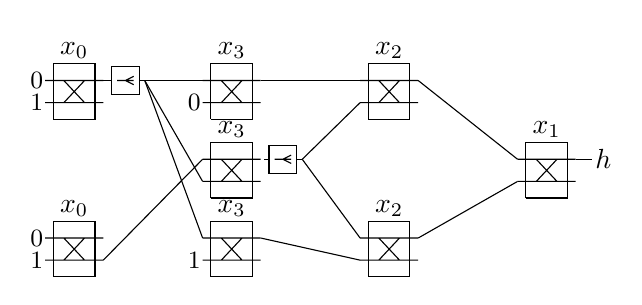
\begin{tikzpicture}
\crossbarat{$x_0$}{0,1}{x0-1}
\crossbarat{$x_0$}{0,-1}{x0-2}
\crossbarat{$x_3$}{2,1}{x3-1}
\crossbarat{$x_3$}{2,0}{x3-2}
\crossbarat{$x_3$}{2,-1}{x3-3}
\crossbarat{$x_2$}{4,1}{x2-1}
\crossbarat{$x_2$}{4,-1}{x2-2}
\crossbarat{$x_1$}{6,0}{x1}

\node[shape=splittergate, xshift=8] (s1) at (x0-1.f) {};
\node[shape=splittergate, xshift=8] (s2) at (x3-2.f) {};

\draw (x0-1.f) -- (s1.in);
\draw (s1.out) -- (x3-1.p);
\draw (s1.out) -- (x3-2.q);
\draw (s1.out) -- (x3-3.p);
\draw (x0-2.g) -- (x3-2.p);
\draw (x3-1.f) -- (x2-1.p);
\draw (s2.out) -- (x2-1.q);
\draw (s2.out) -- (x2-2.p);
\draw (x3-3.f) -- (x2-2.q);
\draw (x2-1.f) -- (x1.p);
\draw (x2-2.f) -- (x1.q);

\node[crossin] at (x0-1.p) {\small $0$};
\node[crossin] at (x0-1.q) {\small $1$};
\node[crossin] at (x0-2.p) {\small $0$};
\node[crossin] at (x0-2.q) {\small $1$};
\node[crossin] at (x3-1.q) {\small $0$};
\node[crossin] at (x3-3.q) {\small $1$};

\node[xshift=1em,inner sep=1pt] (f) at (x1.f) {$h$};

\draw (x1.f) -- (f);
\end{tikzpicture}}
\caption{Direct BDD-based synthesis with shared node optimization}\label{fig:direct-bdd-h}
\end{figure}

In terms of fraction, the above two examples illustrate the dilemma of optimizing contradictory objectives. To investigate the effect of shared node minimization in direct BDD-based synthesis, a detailed analysis through experimental evaluation is presented in Section~\ref{sec:results}.

%\subsection{Reverse BDD-based Synthesis with One-path Minimization}
\subsection{Reducing Gates in Splitter-Free Circuits}

In case of reverse BDD-based synthesis, the original BDD for a given function is minimized with respect to the number of one-paths. Like shared node minimization, one-path reduction is also achieved using the approach reported in~\cite{ShirinzadehSD15}. %evolutionary algorithm. 
After reducing the number of one-paths, the resulting BDD is mapped into an optical circuits using reverse BDD approach. Such optimized BDD structure results in smaller realizations of optical circuits. This is illustrated again by means of an example.  

\begin{example}
Consider the multi-output functions~$f:\B^4\rightarrow\B^2$ with 
\begin{align*}
f_0 &=x_0x_1\bar{x}_2+x_0x_1x_2x_3+x_0\bar{x}_1x_3+\bar{x}_0\bar{x}_1x_2\bar{x}_3+
\bar{x}_0x_1x_2 \quad\text{and}\\
f_1 &=x_0\bar{x}_1x_2x_3+x_0\bar{x}_1\bar{x}_2\bar{x}_3+x_0x_1\bar{x}_2\bar{x}_3+
\bar{x}_0\bar{x}_1x_2
\end{align*}
The corresponding BDDs are shown in Fig.~\ref{fig:rev-bdd-before-path-min}. Considering both BDDs together, there are 16 nodes and 9 one-paths. The resulting optical circuits (depicted in Fig.~\ref{fig:rev-bdd-circ-before-path-min}) contain crossbar gates equal to the number of BDD nodes. After minimizing the number of one-paths, the BDDs appeared in Fig.~\ref{fig:rev-bdd-after-path-min} contains 12 nodes and 7 one-paths in total. This leads to the optical circuits composed of 12 crossbar gates as shown in Fig.~\ref{fig:rev-bdd-circ-after-path-min}. Therefore, this optimization decreases the total gate count from 16 to 12, and eventually, results in a much better circuit size -- especially for multi-output functions. 
\end{example}

\begin{figure}[!h]
\centering
\subfloat[Original BDDs\label{fig:rev-bdd-before-path-min}]{\begin{tikzpicture}[every node/.style={draw,circle,inner
sep=2},scale=.6]
\begin{scope}
\node (f0) {$x_0$} 
	child {
		node (x1-1) {$x_1$}
		child {
			node[xshift=-20] (x2-1) {$x_2$}
			child {
			    node[xshift=30] (x3-1){$x_3$}
			    child[solid] {
			      node[rectangle, xshift=20] (oneterm) {$1$}
			    }  
			}  
		}
	}
	child[dashed] {
	   node[solid, xshift=20] (x1-2) {$x_1$}
	   child[dashed] {
		 node[solid] (x2-2) {$x_2$}
		 child[solid] {
			 node (x3-2) {$x_3$}
		 }
	   }	
	   child[solid] {
		  node (x2-3) {$x_2$}
		}
	};
		
		
\draw[dashed] (x1-1) -- (x3-1);
\draw[dashed] (x2-1) edge[in=160, out=280] (oneterm);
\draw[dashed] (x3-2) -- (oneterm);
\draw (x2-3) edge[in=40,out=260] (oneterm);

\node[above of=f0, draw=none,yshift=-3,inner sep=0] (f0l) {$f_0$};

\draw (f0) -- (f0l);
\end{scope}
%\end{tikzpicture}}\hspace{.5cm}
%\subfloat[BDD\label{fig:bdd}]{\begin{tikzpicture}[every node/.style={draw,circle,inner
%sep=2},scale=.6]
\begin{scope}[xshift = 6.2cm]
\node (f1) {$x_0$} 
	child {
		node (x1-1) {$x_1$}
		child[dashed] {
			node[solid] (x2-1) {$x_2$}
			child[solid] {
			    node (x3-1){$x_3$}
			    child {
			      node[rectangle,xshift=30] (oneterm) {$1$}
			     }
			}
			child {
			    node[solid] (x3-2) {$x_3$}
			}    
		}
		child {
			node (x2-2) {$x_2$}
		}
    }			
	child[dashed] {
	  node[solid, xshift=20] (x1-2) {$x_1$}
	   child[dashed] {
		  node[solid] (x2-3) {$x_2$}
	   }
    };
		
\draw[dashed] (x3-2) -- (oneterm);
\draw (x2-3) -- (oneterm);
\draw[dashed] (x2-2) -- (x3-2);

\node[above of=f1, draw=none,yshift=-3,inner sep=0] (f1l) {$f_1$};

\draw (f1) -- (f1l);
\end{scope}
\end{tikzpicture}}\hspace{2cm}
\subfloat[Resulting circuits\label{fig:rev-bdd-circ-before-path-min}]{
\resizebox{\textwidth}{!}{
\begin{tikzpicture}
\begin{scope}
\crossbarat{$x_0$}{0,1}{x0}
\crossbarat{$x_1$}{1.5,1.7}{x1-1}
\crossbarat{$x_1$}{1.5,0.5}{x1-2}
\crossbarat{$x_2$}{3,2}{x2-1}
\crossbarat{$x_2$}{3,0.5}{x2-2}
\crossbarat{$x_2$}{3.4,-0.5}{x2-3}
\crossbarat{$x_3$}{5,1.2}{x3-1}
\crossbarat{$x_3$}{4.8,-0.5}{x3-2}

\node[shape=combinergate] (c1) at (4,1.2) {};
\node[shape=combinergate] (c2) at (6.3,0.65) {};

\draw (x0.f) -- (x1-1.q);
\draw (x0.g) -- (x1-2.q);
\draw (x1-1.f) -- (x2-1.q);
\draw (x1-2.f) -- (x2-2.q);
\draw (x1-2.g) -- (x2-3.q);
\draw (x2-1.g) -- (c1.in);
\draw (x1-1.g) -- (c1.in);
\draw (c1.out) -- (x3-1.q);
\draw (x2-3.f) -- (x3-2.q);
\draw (x3-1.f) -- (c2.in);
\draw (x3-2.g) -- (c2.in); 
\draw (x2-2.f) -- (c2.in);
\draw (x2-1.f) edge[in=80,out=360] (c2.in);

\node[crossin] at (x0.p) {\small $0$};
\node[crossin] at (x0.q) {\small $1$};
\node[crossin] at (x1-1.p) {\small $0$};
\node[crossin] at (x1-2.p) {\small $0$};
\node[crossin] at (x2-1.p) {\small $0$};
\node[crossin] at (x2-2.p) {\small $0$};
\node[crossin] at (x2-3.p) {\small $0$};
\node[crossin] at (x3-1.p) {\small $0$};
\node[crossin] at (x3-2.p) {\small $0$};

\node[xshift=1em,inner sep=1pt] (f0) at (c2.out) {$f_0$};

\draw (f0) -- (c2.out);
\end{scope}
%\end{tikzpicture}}\hspace{1cm}
%\subfloat[Obtained circuit\label{fig:bdd_circ}]{
%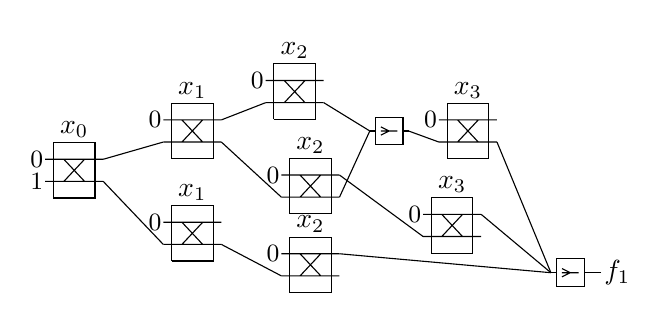
\begin{tikzpicture}
\begin{scope}[xshift = 8cm]
\crossbarat{$x_0$}{0,1}{x0}
\crossbarat{$x_1$}{1.5,1.5}{x1-1}
\crossbarat{$x_1$}{1.5,0.2}{x1-2}
\crossbarat{$x_2$}{2.8,2}{x2-1}
\crossbarat{$x_2$}{3,0.8}{x2-2}
\crossbarat{$x_2$}{3,-0.2}{x2-3}
\crossbarat{$x_3$}{5,1.5}{x3-1}
\crossbarat{$x_3$}{4.8,0.3}{x3-2}

\node[shape=combinergate] (c1) at (4,1.5) {};
\node[shape=combinergate] (c2) at (6.3,-0.3) {};

\draw (x0.f) -- (x1-1.q);
\draw (x0.g) -- (x1-2.q);
\draw (x1-1.f) -- (x2-1.q);
\draw (x1-1.g) -- (x2-2.q);
\draw (x1-2.g) -- (x2-3.q);
\draw (x2-1.g) -- (c1.in);
\draw (x2-2.g) -- (c1.in);
\draw (x2-2.f) -- (x3-2.q);
\draw (c1.out) -- (x3-1.q);
\draw (x2-3.f) -- (c2.in);
\draw (x3-2.f) -- (c2.in);
\draw (x3-1.g) -- (c2.in);

\node[crossin] at (x0.p) {\small $0$};
\node[crossin] at (x0.q) {\small $1$};
\node[crossin] at (x1-1.p) {\small $0$};
\node[crossin] at (x1-2.p) {\small $0$};
\node[crossin] at (x2-1.p) {\small $0$};
\node[crossin] at (x2-2.p) {\small $0$};
\node[crossin] at (x2-3.p) {\small $0$};
\node[crossin] at (x3-1.p) {\small $0$};
\node[crossin] at (x3-2.p) {\small $0$};

\node[xshift=1em,inner sep=1pt] (f1) at (c2.out) {$f_1$};

\draw (f1) -- (c2.out);
\end{scope}
\end{tikzpicture}}}\hspace{1cm}
\subfloat[BDDs with minimized one-paths\label{fig:rev-bdd-after-path-min}]{\begin{tikzpicture}[every node/.style={draw,circle,inner
sep=2},scale=.6]
\begin{scope}
\node (f0) {$x_0$} 
	child[dashed] {
		node[solid] (x3-1) {$x_3$}
		  child[solid] {
			 node[xshift=-20] (x1-1) {$x_1$}
			  child {
			     node[xshift=20] (x2-1){$x_2$}
			     child {
			        node[rectangle,xshift=20] (oneterm) {$1$}
			     }   
			  }
		   }
	 }	   	  
	 child {
		node (x3-2) {$x_3$}
		child[dashed] {
		   node[solid] (x1-2) {$x_1$}
		   child[solid] {
		      node (x2-2) {$x_2$}
		   }   
		}      
	};    
			  	
\draw[dashed] (x3-1) -- (x2-1);
\draw (x3-2) edge[in=45,out=300] (oneterm);
\draw[dashed] (x2-2) -- (oneterm);

\node[above of=f0, draw=none,yshift=-3,inner sep=0] (f0l) {$f_0$};

\draw (f0) -- (f0l);
\end{scope}
%\end{tikzpicture}}\hspace{.5cm}
%\subfloat[BDD\label{fig:bdd}]{\begin{tikzpicture}[every node/.style={draw,circle,inner
%sep=2},scale=.6]
\begin{scope}[xshift = 6cm]
\node (f1) {$x_0$} 
	child {
		node (x3) {$x_3$}
		child[dashed] {
			node[solid,yshift=-20] (x2-2) {$x_2$}
		}
	}		
	child[dashed] {
	     node[solid,yshift=-20] (x1){$x_1$}
		 child {
			 node[solid] (x2-1) {$x_2$}
			  child[solid] {
			     node[rectangle,xshift=-10] (oneterm) {$1$}
			  }
		  }
	};	  
		
\draw[dashed] (x2-2) -- (oneterm);
\draw (x3) -- (x1);

\node[above of=f1, draw=none,yshift=-3,inner sep=0] (f1l) {$f_1$};

\draw (f1) -- (f1l);
\end{scope}
\end{tikzpicture}}\hspace{.5cm}
\subfloat[Resulting circuits\label{fig:rev-bdd-circ-after-path-min}]{
\resizebox{\textwidth}{!}{
\begin{tikzpicture}
\begin{scope}
\crossbarat{$x_0$}{0,0}{x0}
\crossbarat{$x_3$}{1.5,1.5}{x3-1}
\crossbarat{$x_3$}{1.5,-0.6}{x3-2}
\crossbarat{$x_1$}{3,1}{x1-1}
\crossbarat{$x_1$}{3,-0.2}{x1-2}
\crossbarat{$x_2$}{4.2,1}{x2-1}
\crossbarat{$x_2$}{5.2,-0.6}{x2-2}

\node[shape=combinergate] (c1) at (4,-0.8) {};
\node[shape=combinergate] (c2) at (6.3,1.65) {};

\draw (x0.f) -- (x3-1.q);
\draw (x0.g) -- (x3-2.q);
\draw (x3-1.g) -- (x1-1.q);
\draw (x3-2.f) -- (x1-2.q);
\draw (x1-1.f) -- (x2-1.q);
\draw (x1-2.f) -- (c1.in);
\draw (x3-2.g) -- (c1.in);
\draw (c1.out) -- (x2-2.q);
\draw (x3-1.f) -- (c2.in);
\draw (x2-1.g) -- (c2.in);
\draw (x2-2.f) -- (c2.in);

\node[crossin] at (x0.p) {\small $0$};
\node[crossin] at (x0.q) {\small $1$};
\node[crossin] at (x3-1.p) {\small $0$};
\node[crossin] at (x3-2.p) {\small $0$};
\node[crossin] at (x1-1.p) {\small $0$};
\node[crossin] at (x1-2.p) {\small $0$};
\node[crossin] at (x2-1.p) {\small $0$};
\node[crossin] at (x2-2.p) {\small $0$};

\node[xshift=1em,inner sep=1pt] (f0) at (c2.out) {$f_0$};

\draw (f0) -- (c2.out);
\end{scope}
%\end{tikzpicture}}\hspace{1cm}
%\subfloat[Obtained circuit\label{fig:bdd_circ}]{
%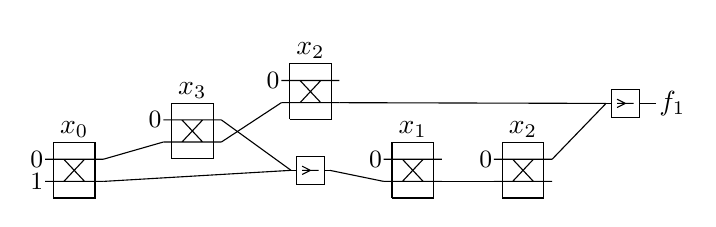
\begin{tikzpicture}
\begin{scope}[xshift = 8cm]
\crossbarat{$x_0$}{0,1}{x0}
\crossbarat{$x_3$}{1.5,1.5}{x3}
\crossbarat{$x_2$}{3,2}{x2-1}
\crossbarat{$x_1$}{4.3,1}{x1}
\crossbarat{$x_2$}{5.7,1}{x2-2}

\node[shape=combinergate] (c1) at (3,1) {};
\node[shape=combinergate] (c2) at (7,1.85) {};

\draw (x0.f) -- (x3.q);
\draw (x3.f) -- (c1.in);
\draw (x0.g) -- (c1.in);
\draw (x3.g) -- (x2-1.q);
\draw (c1.out) -- (x1.q);
\draw (x1.g) -- (x2-2.q);
\draw (x2-1.g) -- (c2.in);
\draw (x2-2.f) -- (c2.in);

\node[crossin] at (x0.p) {\small $0$};
\node[crossin] at (x0.q) {\small $1$};
\node[crossin] at (x3.p) {\small $0$};
\node[crossin] at (x2-1.p) {\small $0$};
\node[crossin] at (x1.p) {\small $0$};
\node[crossin] at (x2-2.p) {\small $0$};
%\node[crossin] at (x2-3.p) {\small $0$};
%\node[crossin] at (x3-1.p) {\small $0$};
%\node[crossin] at (x3-2.p) {\small $0$};

\node[xshift=1em,inner sep=1pt] (f1) at (c2.out) {$f_1$};

\draw (f1) -- (c2.out);
\end{scope}
\end{tikzpicture}}}
\caption{Reverse BDD-based synthesis with one-path optimization}\label{fig:rev-bdd-one-path}
\end{figure}

In the next section, we evaluate the effect of these BDD optimization in resulting optical circuits.

\section{Experimental Evaluation}\label{sec:bdd-min-results}

We have implemented the shared node minimization and one-path minimization approaches in C++ on top of the CUDD package. Experiments are conducted over a set of benchmarks taken from the LGSynth library. All experiments are carried out on a 2.6 GHz Intel Core i5 machine with 8 GB of memory running Linux. The following sections provide details of the experimental evaluations. 

%\subsection{Effect of Shared Node Minimization to the Direct BDD-based Synthesis}
\subsection{Effect of Splitter Minimization to Gate-Efficient BDD-based Synthesis}

Table~\ref{tab:direct-bdd-results} lists the results obtained before and after applying shared node minimization. The first column shows the details of the considered benchmarks, i.e. the name of the benchmark (name) as well as the number of primary inputs and outputs (PI/PO). The next column includes $G_{orig}$, $G_{opt}$, i.e. the number of crossbar gates obtained before and after BDD minimization as well as the percentage of reduction in the number of gates. Likewise, the following columns provide the statistics on the splitter count (i.e. number of splitters) and worst fraction.

As expected, the optimized BDD reduces the number of splitters by just over $52\%$, on average. Furthermore, applying shared node minimization, allows for circuits with $34.7\%$ less number of crossbar gates on average -- in the best case (\emph{apex2}), even reductions of over $92\%$ are obtained. In the worst cases (e.g.~\emph{cps,cm151a,tial}), the number of crossbar gates increases, however, the amount of increase is not significant.

The shared node reduction has a mixed influence on the overall fraction of the optical circuits. More precisely, in case of $24$ benchmarks (i.e. from \emph{apex2} to \emph{5xp1}), a decrease in the number of shared nodes results a several orders of magnitude reductions in fraction. This includes the cases where fraction remains same after shared node reduction. In contrast, there are $13$ benchmarks (from \emph{frg1} to \emph{dist}) for which fractions become worse although the amount of shared nodes in the BDD has been minimized (similar as discussed in Example~\ref{ex:increase_in_fraction} before). Nevertheless, from this analysis, one can note that the amount of fraction still decreases significantly in most of the cases. 

\begin{table}[t]
\centering
\caption{Effect of shared node minimization to the direct BDD-based synthesis}
\resizebox{!}{6cm}{
\begin{tabular}{rr|rrr|rrr|rrr}
\multicolumn{2}{c|}{Function} & \multicolumn{3}{c|}{\# of crossbar gates} & \multicolumn{3}{c|}{\# of splitters} & \multicolumn{3}{c}{Fraction} \\ 
name & PI/PO & $G_{orig}$ & $G_{opt}$ & reduc. & $BS_{orig}$ &  $BS_{opt}$ & reduc. & $F_{orig}$ & $F_{opt}$ & reduc. \\ \hline
apex2 & 39/3 & 7102 & 527 & 92.6\% & 1756 & 120 & 93.2\% & 2099380224 & 535080 & 100.0\% \\ 
cordic & 23/2 & 80 & 85 & -6.3\% & 29 & 27 & 6.9\% & 10240 & 10240 & 0.0\% \\ 
cm151a & 19/9 & 93 & 82 & 11.8\% & 14 & 5 & 64.3\% & 16 & 8 & 50.0\% \\ 
cm163a & 16/13 & 50 & 54 & -8.0\% & 8 & 3 & 62.5\% & 60 & 16 & 73.3\% \\ 
pcler8 & 16/5 & 58 & 35 & 39.7\% & 16 & 3 & 81.3\% & 4 & 4 & 0.0\% \\ 
pdc & 16/40 & 705 & 703 & 0.3\% & 124 & 116 & 6.5\% & 18900 & 6750 & 64.3\% \\ 
t481 & 16/1 & 32 & 32 & 0.0\% & 11 & 11 & 0.0\% & 1296 & 1296 & 0.0\% \\ 
cmb & 16/4 & 47 & 48 & -2.1\% & 1 & 1 & 0.0\% & 2 & 2 & 0.0\% \\ 
ryy6 & 16/1 & 23 & 17 & 26.1\% & 7 & 4 & 42.9\% & 96 & 40 & 58.3\% \\ 
in0 & 15/11 & 526 & 342 & 35.0\% & 143 & 40 & 72.0\% & 99792 & 1140 & 98.9\% \\ 
f51m & 14/8 & 1219 & 489 & 59.9\% & 407 & 102 & 74.9\% & 244992 & 3456 & 98.6\% \\ 
alu4 & 14/8 & 1352 & 763 & 43.6\% & 339 & 145 & 57.2\% & 1188000 & 36000 & 97.0\% \\ 
misex3c & 14/14 & 847 & 479 & 43.4\% & 202 & 101 & 50.0\% & 367200 & 15400 & 95.8\% \\ 
misex3 & 14/14 & 1301 & 722 & 44.5\% & 349 & 129 & 63.0\% & 50319360 & 823680 & 98.4\% \\ 
tial & 14/8 & 1354 & 796 & 41.2\% & 397 & 182 & 54.2\% & 1175040 & 756000 & 35.7\% \\ 
table3 & 14/14 & 941 & 909 & 3.4\% & 212 & 158 & 25.5\% & 355829760 & 16329600 & 95.4\% \\ 
alu2 & 10/6 & 257 & 203 & 21.0\% & 65 & 33 & 49.2\% & 11616 & 630 & 94.6\% \\ 
alu3 & 10/8 & 143 & 72 & 49.7\% & 40 & 13 & 67.5\% & 168 & 144 & 14.3\% \\ 
urf2 & 8/8 & 386 & 395 & -2.3\% & 80 & 58 & 27.5\% & 3264 & 2552 & 21.8\% \\ 
duke2 & 22/29 & 976 & 445 & 54.4\% & 248 & 60 & 75.8\% & 545376 & 1350 & 99.8\% \\ 
clip & 9/5 & 254 & 109 & 57.1\% & 63 & 27 & 57.1\% & 1936 & 288 & 85.1\% \\ 
sao2 & 10/4 & 154 & 100 & 35.1\% & 30 & 17 & 43.3\% & 10080 & 384 & 96.2\% \\ 
vg2 & 25/8 & 1059 & 359 & 66.1\% & 302 & 15 & 95.0\% & 10000000 & 499200 & 95.0\% \\ 
5xp1 & 7/10 & 88 & 84 & 4.5\% & 29 & 9 & 69.0\% & 288 & 81 & 71.9\% \\ 
frg1 & 28/3 & 203 & 114 & 43.8\% & 26 & 13 & 50.0\% & 120 & 1200 & -900.0\% \\ 
spla & 16/46 & 681 & 699 & -2.6\% & 114 & 103 & 9.6\% & 6480 & 43200 & -566.7\% \\ 
urf6 & 15/15 & 4486 & 4498 & -0.3\% & 991 & 890 & 10.2\% & 10769760 & 23814000 & -121.1\% \\ 
ham15 & 15/15 & 119 & 140 & -17.6\% & 72 & 42 & 41.7\% & 1024 & 2560 & -150.0\% \\ 
cu & 14/11 & 65 & 58 & 10.8\% & 10 & 5 & 50.0\% & 10 & 20 & -100.0\% \\ 
urf4 & 11/11 & 3037 & 3046 & -0.3\% & 273 & 261 & 4.4\% & 63296 & 70560 & -11.5\% \\ 
dk17 & 10/11 & 127 & 71 & 44.1\% & 19 & 10 & 47.4\% & 84 & 432 & -414.3\% \\
ex1010 & 10/10 & 1079 & 1078 & 0.1\% & 168 & 157 & 6.5\% & 370944 & 399840 & -7.8\% \\
urf3 & 10/10 & 1322 & 1331 & -0.7\% & 223 & 198 & 11.2\% & 47658 & 94815 & -98.9\% \\  
apex4 & 9/19 & 1021 & 1080 & -5.8\% & 173 & 160 & 7.5\% & 67932 & 349440 & -414.4\% \\
urf1 & 9/9 & 741 & 761 & -2.7\% & 131 & 125 & 4.6\% & 12600 & 30380 & -141.1\% \\ 
urf5 & 9/9 & 425 & 363 & 14.6\% & 71 & 50 & 29.6\% & 8316 & 15232 & -83.2\% \\ 
dist & 8/5 & 195 & 174 & 10.8\% & 38 & 29 & 23.7\% & 1440 & 3420 & -137.5\% \\
\hline
\end{tabular}}
\label{tab:direct-bdd-results}
\end{table}


%\subsection{Effect of One-path Minimization to the Reverse BDD-based Synthesis}
\subsection{Effect of Gate Minimization to Splitter-Free BDD-based Synthesis}

The results are summarized in Table~\ref{tab:reverse-bdd-result}. The first column provides the details on considered functions, i.e. the name of the benchmark (name) and the number of primary inputs and outputs (PI/PO). The next column reports the number of crossbar gates obtained from original~$G_{orig}$ and optimized~$G_{opt}$ reverse BDD-based approach as well as the percentage of reductions in number of gates. In a similar fashion, the following column provides the number of combiners for each synthesized benchmark.

In total,  one-path minimization reduces the number of gates by $32\%$. The reduction in number of gates is positive for all benchmarks except three: \emph{cordic, pdc, urf6}. For these three benchmarks, the optimization increases the gate count. Besides the number of gates, Table~\ref{tab:reverse-bdd-result} presents statistics on the number of combiners. The analysis shows that the number of combiners is reduced under this optimization. In fact, the average reduction of $65.9\%$ is obtained with $96.9\%$ as the best case (\emph{apex2}) reduction. On the other hand, there are four benchmarks (\emph{cordic,ham15,apex4,urf4}) for which this optimization results in a small increase in the combiner count. In summary, it can be concluded that minimizing the one-paths in the BDD leads to better realizations of optical circuits, both in terms of crossbar gates and combiners.    

\begin{table}[t]
\centering
\caption{Reverse-BDD based synthesis: unoptimized vs. optimized}
\resizebox{!}{6cm}{
\begin{tabular}{rr|rrr|rrr}
\multicolumn{2}{c|}{Function} & \multicolumn{3}{c|}{\# of crossbar gates} & \multicolumn{3}{c}{\# of combiners} \\ 
name & PI/PO & $G_{orig}$ & $G_{opt}$ & reduc. & $BC_{orig}$ & $BC_{opt}$ & reduc. \\ \hline
apex2 & 39/3 & 7182 & 683 & 90.5\% & 6176 & 192 & 96.9\% \\ 
frg1 & 28/3 & 203 & 113 & 44.3\% & 189 & 28 & 85.2\% \\ 
cordic & 23/2 & 82 & 173 & -111.0\% & 64 & 75 & -17.2\% \\ 
cm151a & 19/9 & 94 & 86 & 8.5\% & 67 & 20 & 70.1\% \\ 
spla & 16/46 & 1090 & 1000 & 8.3\% & 316 & 169 & 46.5\% \\ 
cm163a & 16/13 & 70 & 65 & 7.1\% & 23 & 10 & 56.5\% \\ 
pcler8 & 16/5 & 59 & 39 & 33.9\% & 29 & 8 & 72.4\% \\ 
pdc & 16/40 & 1118 & 1182 & -5.7\% & 413 & 202 & 51.1\% \\ 
t481 & 16/1 & 32 & 32 & 0.0\% & 29 & 12 & 58.6\% \\ 
cmb & 16/4 & 48 & 48 & 0.0\% & 2 & 2 & 0.0\% \\ 
ryy6 & 16/1 & 23 & 20 & 13.0\% & 20 & 6 & 70.0\% \\ 
ham15 & 15/15 & 183 & 154 & 15.8\% & 87 & 88 & -1.1\% \\ 
in0 & 15/11 & 625 & 412 & 34.1\% & 307 & 73 & 76.2\% \\ 
f51m & 14/8 & 1605 & 529 & 67.0\% & 683 & 137 & 79.9\% \\ 
alu4 & 14/8 & 1534 & 726 & 52.7\% & 438 & 175 & 60.0\% \\ 
misex3c & 14/14 & 970 & 601 & 38.0\% & 556 & 129 & 76.8\% \\ 
misex3 & 14/14 & 1976 & 834 & 57.8\% & 1320 & 187 & 85.8\% \\ 
tial & 14/8 & 1677 & 747 & 55.5\% & 726 & 182 & 74.9\% \\ 
cu & 14/11 & 97 & 75 & 22.7\% & 12 & 6 & 50.0\% \\ 
table3 & 14/14 & 1996 & 1498 & 24.9\% & 618 & 279 & 54.9\% \\ 
alu2 & 10/6 & 286 & 213 & 25.5\% & 87 & 48 & 44.8\% \\ 
alu3 & 10/8 & 159 & 83 & 47.8\% & 91 & 24 & 73.6\% \\ 
apex4 & 9/19 & 1609 & 1513 & 6.0\% & 299 & 331 & -10.7\% \\ 
dist & 8/5 & 247 & 218 & 11.7\% & 70 & 51 & 27.1\% \\ 
dk17 & 10/11 & 162 & 93 & 42.6\% & 38 & 15 & 60.5\% \\ 
ex1010 & 10/10 & 1614 & 1605 & 0.6\% & 318 & 299 & 6.0\% \\ 
urf1 & 9/9 & 1030 & 1018 & 1.2\% & 202 & 189 & 6.4\% \\ 
urf2 & 8/8 & 548 & 527 & 3.8\% & 126 & 103 & 18.3\% \\ 
urf3 & 10/10 & 1881 & 1810 & 3.8\% & 313 & 300 & 4.2\% \\ 
urf4 & 11/11 & 4652 & 4571 & 1.7\% & 859 & 863 & -0.5\% \\ 
urf5 & 9/9 & 537 & 437 & 18.6\% & 135 & 96 & 28.9\% \\ 
urf6 & 15/15 & 6774 & 6945 & -2.5\% & 1870 & 1392 & 25.6\% \\ 
duke2 & 22/29 & 1355 & 557 & 58.9\% & 390 & 103 & 73.6\% \\ 
clip & 9/5 & 280 & 118 & 57.9\% & 100 & 44 & 56.0\% \\ 
sao2 & 10/4 & 182 & 111 & 39.0\% & 52 & 30 & 42.3\% \\ 
vg2 & 25/8 & 1194 & 233 & 80.5\% & 364 & 53 & 85.4\% \\ 
5xp1 & 7/10 & 113 & 98 & 13.3\% & 58 & 34 & 41.4\% \\ \hline
\end{tabular}}
\label{tab:reverse-bdd-result}
\end{table}

\section{Discussion}

\newpage

\section{Chapter Contribution and Summary\sectionmark{Summary}}\label{sec:bdd-summary}

This chapter provides an overview of existing BDD-based synthesis approaches for optical circuits.
The review identifies the potential shortcomings of respective solutions for the synthesis of optical circuits based on BDDs. Motivated by that, the chapter outlines how BDD optimization can be adjusted in order to explicitly address these shortcomings. In particular, observation is made on how the number of shared nodes and the number of one-paths affect the results depending on the applied synthesis scheme. Based on this, optimization schemes are proposed which significantly address the drawbacks of the previously proposed solutions.

This way, the chapter provides a comprehensive consideration of BDD-based synthesis of optical circuits covering previous work as well as proposing new optimization. Experimental evaluations confirmed that the proposed optimization yields better circuit realizations. Depending on the design objective either improvements in the number of gates of up to $33\%$ on average or improvements of several orders of magnitudes in the worst case fraction can be reported. This eventually yields logic designs which fit much better to currently known and possible future technological constraints.

%%%%%%%%%%%%%%%%%%%%%%%%%%%%%%%%%%%%%%%%%%%%%%%%%%%%%%%%%%%%%%%%%%%%%%%%%%%%%%%%%%%%
\chapter{OR-Inverter Graphs for Synthesis of Optical Circuits}~\label{ch:oig-opt}

\section{Motivation}

\newpage

\section{OR-Inverter Graph}

\newpage

\section{Proposed approach}

\subsection{Transformation of AIG into OIG}

\newpage

\subsection{Gate-efficient Synthesis Flow}

\newpage

\subsection{Splitter-free Synthesis Flow}

\newpage

\section{Experimental Evaluation}

\newpage

\section{Discussion}

\newpage

\section{Chapter Contribution and Summary}

\newpage

%%%%%%%%%%%%%%%%%%%%%%%%%%%%%%%%%%%%%%%%%%%%%%%%%%%%%%%%%%%%%%%%%%%%%%%%%%%%%%%%%%%%
%\chapter{Optical Synthesis of Symmetric Function}~\label{ch:optical-symmetric}

%\section{Gate-Efficient Design}

%\newpage

%\section{Splitter-Free Design}

%\newpage

%\section{Experimental Evaluation}

%\newpage

%\section{Discussion}

%\newpage

%\section{Chapter Contribution and Summary}

%\newpage

%%%%%%%%%%%%%%%%%%%%%%%%%%%%%%%%%%%%%%%%%%%%%%%%%%%%%%%%%%%%%%%%%%%%%%%%%%%%%%%%%%%%
%\chapter{Background}~\label{ch:background}

%\section{Reversible Computing}




%\section{Optical Computing}



%\section{Boolean Function Representation}

%\subsection{Two-Level Representation}

%\subsubsection{Sum-of-Products}

%\newpage

%\subsubsection{Exclusive-Sum-of-Products}

%\newpage

%\subsection{Binary Decision Diagram}

%\newpage

%\subsubsection{AND-Inverter Graph}

%\newpage

%\section{Symmetric Boolean Function}

%\newpage

%%%%%%%%%%%%%%%%%%%%%%%%%%%%%%%%%%%%%%%%%%%%%%%%%%%%%%%%%%%%%%%%%%%%%%%%%%%%%%%%%%%%
\part{Reversible Computing}~\label{part:reversible}
\chapter{Background on Reversible Computing}

\section{Reversible Functions}

\newpage

\section{Reversible Circuits}

\newpage

\section{Applied Cost Metrics}

\newpage

\section{Related Work}

\newpage

%%%%%%%%%%%%%%%%%%%%%%%%%%%%%%%%%%%%%%%%%%%%%%%%%%%%%%%%%%%%%%%%%%%%%%%%%%%%%%%%%%%%%%%%
\chapter{Reversible Synthesis of Symmetric Boolean Function}~\label{ch:rev-synth-symm}

\section{Symmetric Boolean Function}

\newpage

\section{Quantum Cost Aware Synthesis}

\newpage

\section{Line Aware Synthesis}

\newpage

\section{Synthesis of Arbitrary Symmetric Boolean Function}

\newpage

\section{Experimental Evaluation}

\newpage

\section{Discussion}

\newpage

\section{Chapter Contribution and Summary}

\newpage


%%%%%%%%%%%%%%%%%%%%%%%%%%%%%%%%%%%%%%%%%%%%%%%%%%%%%%%%%%%%%%%%%%%%%%%%%%%%%%%%%%%%
\part{Quaternary Quantum Computing}~\label{part:quaternary-quantum}
\chapter{Background on Quaternary Quantum Computing}

\section{Quantum Quaternary Logic}

\subsection{GF(4) Arithmetic}

\newpage

\subsection{Quantum Quaternary Circuits}

\newpage

\subsection{Applied Cost Metrics}

\newpage

\section{Existing Design Schemes}

\newpage

%%%%%%%%%%%%%%%%%%%%%%%%%%%%%%%%%%%%%%%%%%%%%%%%%%%%%%%%%%%%%%%%%%%%%%%%%%%%%%%%%%%%%%%%%
\chapter{Quantum Quaternary Synthesis of Symmetric Boolean Function}~\label{ch:quaternary-symm}

\section{Quaternary Interpretation of Symmetric Boolean Function}

\newpage

\section{Proposed Synthesis and Optimization Technique}

\subsection{Design of Quaternary Quantum Array}

\newpage

\subsection{Optimization of Quaternary Quantum Array}

\newpage

\section{Synthesis of Arbitrary Symmetric Boolean Function}

\newpage

\section{Experimental Evaluation}

\newpage

\section{Discussion}

\newpage

\section{Chapter Contribution and Summary}

\newpage

%%%%%%%%%%%%%%%%%%%%%%%%%%%%%%%%%%%%%%%%%%%%%%%%%%%%%%%%%%%%%%%%%%%%%%%%%%%%%%%%%%%%%
\chapter{Conclusion and future work}~\label{ch:conclusion}

%\todo[inline]{write first draft}
\newpage

%%%%%%%%%%%%%%%%%%%%%%%%%%%%%%%%%%%%%%%%%%%%%%%%%%%%%%%%%%%%%%%%%%%%%%%%%%%%%%%%%%%%%
\bibliographystyle{unsrt}
\bibliography{phd_thesis}
\end{document}